\chapter{Electrons in crystals}\label{chap:3}

A plane wave with the typical momentum of a valence electron, $q_0 = \SI{3.73}{keV}$ (\cref{sec:1.3}), has a wavelength of \SI{3.3}{\angstrom}, not much longer than the \SI{2.35}{\angstrom} bond between two silicon atoms. Dark matter that scatters on electrons with such momentum transfers sees the arrangement of the atoms. \Cref{chap:2} reduced every scattering rate to matrix elements of the density operator $n_e(\vect{q})$ between states of the target and collected them in the dynamic structure factor, but it left open what those states are. The free electron gas of \cref{sec:2.5} has the right density and the right momentum scale, $k_{\mathrm{F}} \approx q_0$, yet it can take up any energy, while the electrons of silicon cannot be excited by less than \SI{1.17}{eV}. The difference comes from the periodic potential of the nuclei. It groups the electron states into bands separated by gaps, it decides which momentum transfers connect which states, and it shapes the wavefunctions on the scale that a few-keV momentum transfer resolves. The threshold of an electron-recoil detector, and how fast its rate grows above threshold, are therefore properties of the electronic structure of the crystal. The computed bands of silicon and GaAs in this chapter are Kohn--Sham bands: density-functional theory turns the Coulomb Hamiltonian of \cref{eq:2.3-HC} into a problem of independent electrons in an effective potential, accurate enough to compute bands and wavefunctions of real materials, but not their gap. By the end of the chapter, along the path of \cref{fig:3-map}, we will have the states of an electron in silicon, the matrix elements of $\ee^{\ii\vect{q}\cdot\vect{r}}$ between them, and the band edges that set the threshold, with the gap corrected.

\begin{figure}[tbp]
  \centering
  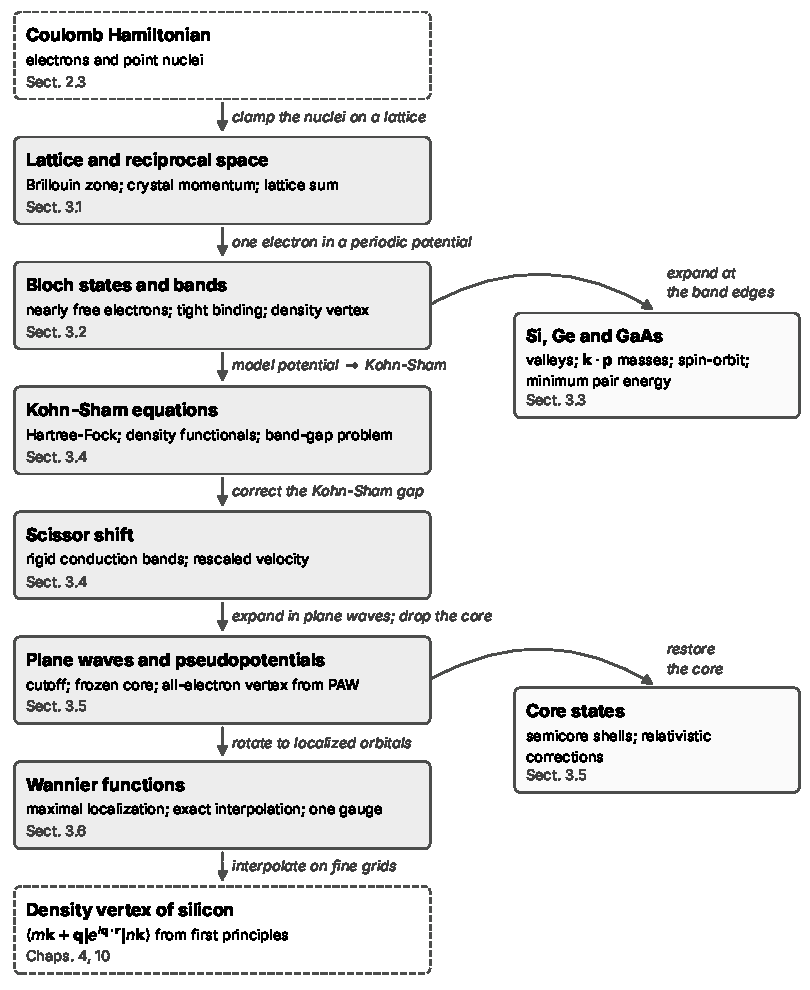
\includegraphics[width=0.85\linewidth]{figures/ch03/map03.pdf}
  \caption{From the Coulomb Hamiltonian to the density vertex of silicon. Clamping the nuclei on a lattice gives reciprocal space and crystal momentum (\cref{sec:3.1}); one electron in a periodic potential gives Bloch bands and the density vertex (\cref{sec:3.2}), whose band edges fix the valleys, masses and minimum pair energy of Si, Ge and GaAs (\cref{sec:3.3}). The Kohn--Sham potential replaces the model potential, and the scissor shift corrects its gap (\cref{sec:3.4}). Dashed boxes: the starting Hamiltonian (\cref{sec:2.3}), the use of the vertex (\cref{chap:4,chap:10}) and the practical calculation of bands and wavefunctions, with plane waves and pseudopotentials, the core restored where large momentum transfers need it (\cref{chap:24}), and Wannier interpolation (\cref{chap:25}).}
  \label{fig:3-map}
\end{figure}

\section{Lattices and reciprocal space}\label{sec:3.1}

A kilogram of silicon holds $2.1\times10^{25}$ atoms, and every one of them sits at a point of a lattice that repeats the same pair of atoms in every direction. The repetition has two consequences that every later rate uses: a crystal conserves momentum only up to a reciprocal-lattice vector, the working definition of \cref{sec:1.3}, and the momenta it can tell apart fill a single cell of reciprocal space, the Brillouin zone. We construct both for the diamond structure of silicon, count the states in the zone, and measure the momentum transfers of \cref{sec:1.3} against the size of the zone. The material is standard, and we follow Refs.~\cite[Chaps.~4--6 and 8]{ashcroft1976solid} and \cite[Chaps.~1--2]{kittel2005introduction}.

Throughout \cref{chap:3,chap:4} the nuclei sit at fixed equilibrium positions: we work with a \emph{static lattice}. The approximation rests on the mass ratio. A silicon nucleus is $M/m_e = \num{5.1e4}$ times heavier than an electron, and the electrons rearrange long before the nuclei have moved appreciably. \Cref{sec:5.1} makes this precise with the Born--Oppenheimer expansion. What the static lattice leaves out are the vibrations themselves, phonons, and their coupling to the electrons, which \cref{chap:5,chap:6} add back.

\subsection{Bravais lattice and basis}

A \emph{Bravais lattice} is the set of points
\begin{equation}
  \vect{R} = n_1\vect{a}_1 + n_2\vect{a}_2 + n_3\vect{a}_3, \qquad n_i \in \mathbb{Z},
  \label{eq:3.1-R}
\end{equation}
generated by three linearly independent \emph{primitive vectors} $\vect{a}_i$. Every lattice vector $\vect{R}$ maps the lattice onto itself. The parallelepiped spanned by the $\vect{a}_i$ is a primitive cell: its translations by all $\vect{R}$ fill space without overlap, and it contains one lattice point. Its volume,
\begin{equation}
  \Omega = \vect{a}_1\cdot(\vect{a}_2\times\vect{a}_3),
  \label{eq:3.1-Omega}
\end{equation}
is the \emph{cell volume}, the only meaning of a bare $\Omega$ in this book (a solid angle always carries a subscript, as in $\dd\Omega_q$). The choice of primitive vectors is not unique, but every primitive cell has the same volume, since each holds one lattice point.

A crystal places a group of atoms, the \emph{basis}, at every lattice point. We label the atoms of the basis by $\kappa = 1, \dots, n_{\mathrm{at}}$ and their positions within the cell by $\vect{\tau}_\kappa$, so that the nuclei sit at
\begin{equation}
  \vect{X}_{\vect{R}\kappa} = \vect{R} + \vect{\tau}_\kappa .
  \label{eq:3.1-X}
\end{equation}
This is the $\kappa$ that labels $Z_\kappa$ and $n_\kappa(\vect{k})$ in \cref{sec:2.3}; two sites of one element still carry different $\kappa$.

Silicon has the \emph{diamond structure} drawn in \cref{fig:3-diamond}. Its Bravais lattice is face-centered cubic (fcc): the corners and face centers of a cube of side $a$, the \emph{lattice constant}. A symmetric choice of primitive vectors joins a corner to the three nearest face centers,
\begin{equation}
  \vect{a}_1 = \frac{a}{2}(0,1,1), \qquad \vect{a}_2 = \frac{a}{2}(1,0,1), \qquad \vect{a}_3 = \frac{a}{2}(1,1,0),
  \label{eq:3.1-fcc}
\end{equation}
and \cref{eq:3.1-Omega} yields $\Omega = a^3/4$: the cube contains four lattice points. The basis consists of two silicon atoms,
\begin{equation}
  \vect{\tau}_1 = 0, \qquad \vect{\tau}_2 = \frac{a}{4}(1,1,1),
  \label{eq:3.1-basis}
\end{equation}
displaced along the cube diagonal by a quarter of its length. Each atom then has four nearest neighbors at the corners of a regular tetrahedron, at the distance $\sqrt3\,a/4$ and with bond angles of \ang{109.47}. These are the four covalent bonds of a silicon atom, one for each valence electron, and \cref{sec:3.2} returns to the $sp^3$ orbitals that form them. Note that the diamond structure is not a Bravais lattice: the environment of an atom at $\vect{\tau}_2$ is that of an atom at $\vect{\tau}_1$ inverted through the bond center, and no lattice vector maps one onto the other.

\begin{figure}[tbp]
  \centering
  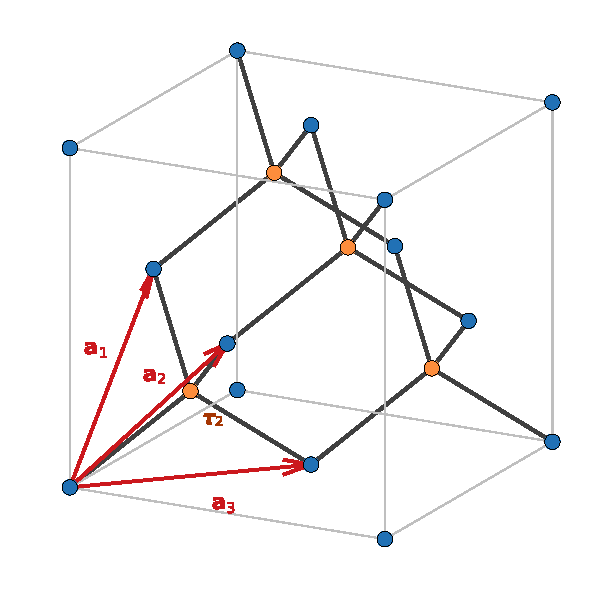
\includegraphics[width=0.55\linewidth]{figures/ch03/fig3_1.pdf}
  \caption{The diamond structure, drawn in a cube of side $a$, the lattice constant. Blue: the face-centered cubic lattice of sites $\vect{R}$ (cube corners and face centers). Orange: the second atom of the basis, at $\vect{R} + \vect{\tau}_2$ with $\vect{\tau}_2 = (a/4)(1,1,1)$; the four inside the cube are shown. Dark lines join nearest neighbors, at a distance $\sqrt3\,a/4$, \SI{2.352}{\angstrom} in silicon ($a = \SI{5.431}{\angstrom}$); each atom is bonded to four others at the corners of a regular tetrahedron. Red arrows: the primitive vectors $\vect{a}_1 = (a/2)(0,1,1)$, $\vect{a}_2 = (a/2)(1,0,1)$, $\vect{a}_3 = (a/2)(1,1,0)$, which span a primitive cell of volume $a^3/4$ containing two atoms. In the zincblende structure (GaAs) the blue and orange sites hold different elements.}
  \label{fig:3-diamond}
\end{figure}

The lattice constant of silicon is $a = \SI{5.431}{\angstrom}$~\cite[lattice parameter of silicon]{mohr2025codata}, or $\num{2.752e-3}\,\mathrm{eV}^{-1}$ in natural units. The cell volume is $\Omega = \SI{40.05}{\angstrom^3}$, the nearest-neighbor distance is \SI{2.352}{\angstrom}, and the cube of side $a$ holds eight atoms. These numbers fix the densities used in the earlier chapters. The atomic density is $8/a^3 = \SI{4.99e22}{cm^{-3}}$, which with the atomic weight 28.0855 yields the mass density \SI{2.33}{g.cm^{-3}} of \cref{sec:1.2}. With four valence electrons per atom, the valence density $32/a^3 = \SI{2.00e23}{cm^{-3}}$ is the one used for the free electron gas of \cref{sec:2.5}. Germanium has the same structure with a lattice constant a few percent larger. Gallium arsenide has the \emph{zincblende structure}, the same lattice and the same $\vect{\tau}_\kappa$, but with gallium at $\vect{\tau}_1$ and arsenic at $\vect{\tau}_2$~\cite[Chap.~4]{ashcroft1976solid}. Since the two sites now differ, the inversion that exchanged them in silicon is no longer a symmetry. As a result GaAs is polar, a property that matters for its phonons (\cref{sec:5.5}). \Cref{sec:3.3} gives the band structures of all three materials.

A first-principles calculation, in density-functional theory (\cref{sec:3.4}), either takes $a$ from experiment or finds it by minimizing the computed total energy of the crystal with respect to $a$ (\cref{app:E.1}). For silicon in the local-density approximation the minimum lies at \SI{5.401}{\angstrom}, \SI{0.5}{\percent} below the measured value~\cite[Sect.~10.2]{ponce2016epw}. A rate is usually computed at the measured $a$. Since band energies depend on $a$, the choice shifts the computed gap, one of the reasons why computed and measured thresholds differ (\cref{sec:3.4}).

\subsection{The reciprocal lattice}

A plane wave $\ee^{\ii\vect{G}\cdot\vect{r}}$ that takes the same value at every lattice point, $\ee^{\ii\vect{G}\cdot\vect{R}} = 1$ for all $\vect{R}$, is the building block of every function with the periodicity of the lattice. The wavevectors $\vect{G}$ with this property are the \emph{reciprocal-lattice vectors}. By \cref{eq:3.1-R} the condition holds for all $\vect{R}$ if and only if $\vect{G}\cdot\vect{a}_i$ is a multiple of $2\pi$ for each $i$. We therefore look for vectors $\vect{b}_j$ with
\begin{equation}
  \vect{a}_i\cdot\vect{b}_j = 2\pi\delta_{ij} .
  \label{eq:3.1-dual}
\end{equation}
They are
\begin{equation}
  \vect{b}_1 = \frac{2\pi}{\Omega}\,\vect{a}_2\times\vect{a}_3, \qquad
  \vect{b}_2 = \frac{2\pi}{\Omega}\,\vect{a}_3\times\vect{a}_1, \qquad
  \vect{b}_3 = \frac{2\pi}{\Omega}\,\vect{a}_1\times\vect{a}_2 .
  \label{eq:3.1-b}
\end{equation}
To check \cref{eq:3.1-dual}, note that $\vect{a}_1\cdot\vect{b}_1 = 2\pi\,\vect{a}_1\cdot(\vect{a}_2\times\vect{a}_3)/\Omega = 2\pi$ by \cref{eq:3.1-Omega}, while $\vect{a}_2\cdot\vect{b}_1$ and $\vect{a}_3\cdot\vect{b}_1$ vanish because a triple product with a repeated vector is zero; the other components follow by cyclic permutation. Since the $\vect{b}_j$ are linearly independent, any wavevector can be written as $\vect{G} = \sum_jm_j\vect{b}_j$ with real $m_j$, and then $\vect{G}\cdot\vect{a}_i = 2\pi m_i$. The condition $\ee^{\ii\vect{G}\cdot\vect{R}} = 1$ thus requires integer $m_i$, and the reciprocal-lattice vectors form a Bravais lattice of their own,
\begin{equation}
  \vect{G} = m_1\vect{b}_1 + m_2\vect{b}_2 + m_3\vect{b}_3, \qquad m_i \in \mathbb{Z},
  \label{eq:3.1-G}
\end{equation}
with primitive vectors $\vect{b}_i$. In the book's convention (\cref{app:A.3}), a function with the periodicity of the lattice is a sum $f(\vect{r}) = \sum_{\vect{G}}f_{\vect{G}}\,\ee^{-\ii\vect{G}\cdot\vect{r}}$ over these vectors, with $f_{\vect{G}} = \Omega^{-1}\int_\Omega\dd^3r\,\ee^{\ii\vect{G}\cdot\vect{r}}f(\vect{r})$ (\cref{eq:A.3-periodic}). The plane wave $\ee^{\ii\vect{G}\cdot\vect{r}}$ is constant on planes perpendicular to $\vect{G}$, and for the shortest $\vect{G}$ in a given direction its wavelength $2\pi/|\vect{G}|$ is the spacing of the lattice planes perpendicular to it.

The volume of the cell spanned by the $\vect{b}_i$ follows from \cref{eq:3.1-b}. With the identity $(\vect{u}\times\vect{v})\times(\vect{u}\times\vect{w}) = \vect{u}\,[\vect{u}\cdot(\vect{v}\times\vect{w})]$ for $\vect{u} = \vect{a}_1$,
\begin{equation*}
  \vect{b}_2\times\vect{b}_3 = \frac{(2\pi)^2}{\Omega^2}\,(\vect{a}_3\times\vect{a}_1)\times(\vect{a}_1\times\vect{a}_2) = \frac{(2\pi)^2}{\Omega^2}\,\vect{a}_1\,[\vect{a}_1\cdot(\vect{a}_2\times\vect{a}_3)] = \frac{(2\pi)^2}{\Omega}\,\vect{a}_1 ,
\end{equation*}
where the sign of the first cross product was reversed to bring $\vect{a}_1$ to the front of both factors, and the sign of the second triple product with it. Then \cref{eq:3.1-dual} gives
\begin{equation}
  \vect{b}_1\cdot(\vect{b}_2\times\vect{b}_3) = \frac{(2\pi)^3}{\Omega} .
  \label{eq:3.1-BZvol}
\end{equation}
A small cell in real space is a large one in reciprocal space, as the Fourier transform requires.

For the fcc vectors of \cref{eq:3.1-fcc}, \cref{eq:3.1-b} yields
\begin{equation}
  \vect{b}_1 = \frac{2\pi}{a}(-1,1,1), \qquad \vect{b}_2 = \frac{2\pi}{a}(1,-1,1), \qquad \vect{b}_3 = \frac{2\pi}{a}(1,1,-1),
  \label{eq:3.1-bfcc}
\end{equation}
as we can confirm directly from \cref{eq:3.1-dual}: for instance, $\vect{a}_1\cdot\vect{b}_1 = \pi(0 + 1 + 1) = 2\pi$ and $\vect{a}_2\cdot\vect{b}_1 = \pi(-1 + 0 + 1) = 0$. These are the primitive vectors of a body-centered cubic lattice. Writing $\vect{G} = (2\pi/a)(h,k,l)$, \cref{eq:3.1-G} reads $h = -m_1 + m_2 + m_3$ and its cyclic permutations, so that $h + k = 2m_3$, $k + l = 2m_1$ and $l + h = 2m_2$. The reciprocal-lattice vectors of the fcc lattice are the vectors $(2\pi/a)(h,k,l)$ with integers $h, k, l$ that are all even or all odd, and every such triple occurs. The integers are the Miller indices of the lattice planes perpendicular to $\vect{G}$, and we write $\vect{G}_{hkl}$. The shortest nonzero vectors are the eight $\vect{G}_{111}$ along the cube diagonals, with $|\vect{G}_{111}| = \sqrt3\,2\pi/a$, followed by the six $\vect{G}_{200}$ along the cube axes, with $|\vect{G}_{200}| = 2\cdot2\pi/a$. In silicon $2\pi/a = \SI{2.28}{keV} = \SI{1.16}{\angstrom^{-1}}$, $|\vect{G}_{111}| = \SI{3.95}{keV}$ and $|\vect{G}_{200}| = \SI{4.57}{keV}$, the scales already met in \cref{sec:1.3,sec:2.4}.

\subsection{The Brillouin zone}

Two wavevectors that differ by a reciprocal-lattice vector give the same phase at every lattice point, $\ee^{\ii(\vect{k} + \vect{G})\cdot\vect{R}} = \ee^{\ii\vect{k}\cdot\vect{R}}$, and a lattice cannot tell them apart. The wavevectors that a crystal can distinguish fill one primitive cell of the reciprocal lattice. The conventional choice of cell is the \emph{first Brillouin zone}, the set of points closer to the origin than to any other reciprocal-lattice vector (\cref{sec:1.3}). The same construction around a point of the direct lattice, the points closer to it than to any other lattice point, is the \emph{Wigner--Seitz cell}, so the first Brillouin zone is the Wigner--Seitz cell of the reciprocal lattice. Its boundary is made of pieces of the planes $\vect{k}\cdot\vect{G} = |\vect{G}|^2/2$ that bisect the vectors $\vect{G}$, and a point on the boundary is equidistant from the origin and from at least one $\vect{G}$. The zone has the full point symmetry of the lattice, which is why it is preferred to the parallelepiped spanned by the $\vect{b}_i$. Both cells tile reciprocal space under translations by $\vect{G}$, and the zone has the volume of \cref{eq:3.1-BZvol}, $(2\pi)^3/\Omega$. For fcc it is $4(2\pi/a)^3$.

\begin{figure}[tbp]
  \centering
  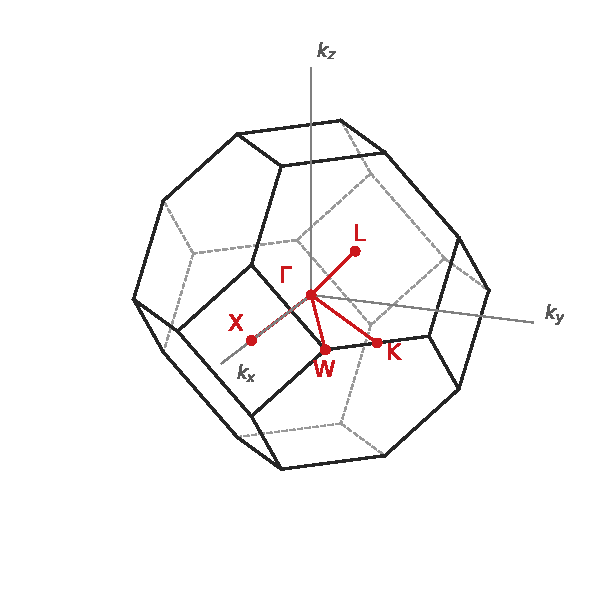
\includegraphics[width=0.52\linewidth]{figures/ch03/fig3_2.pdf}
  \caption{The first Brillouin zone of the face-centered cubic lattice, a truncated octahedron with eight hexagonal faces, which bisect the vectors $\vect{G}_{111} = (2\pi/a)(\pm1,\pm1,\pm1)$, and six square faces, which bisect $\vect{G}_{200} = (2\pi/a)(\pm2,0,0)$ and its permutations. Dashed edges are hidden. The high-symmetry points, in units of $2\pi/a$, are $\mathrm{\Gamma} = (0,0,0)$, $\mathrm{X} = (1,0,0)$, $\mathrm{L} = (\tfrac12,\tfrac12,\tfrac12)$, $\mathrm{K} = (\tfrac34,\tfrac34,0)$ and $\mathrm{W} = (1,\tfrac12,0)$; their distances from $\mathrm{\Gamma}$ are 1, 0.866, 1.061 and 1.118, or 2.28, 1.98, 2.42 and \SI{2.55}{keV} for silicon ($a = \SI{5.431}{\angstrom}$). The zone volume is $4(2\pi/a)^3 = (2\pi)^3/\Omega$.}
  \label{fig:3-bz}
\end{figure}

For the fcc lattice the zone is the truncated octahedron of \cref{fig:3-bz}. The planes that bisect the eight $\vect{G}_{111}$ cut out an octahedron, $|k_x| + |k_y| + |k_z| \le \tfrac32(2\pi/a)$, and the planes that bisect the six $\vect{G}_{200}$, $|k_x|, |k_y|, |k_z| \le 2\pi/a$, cut off its six corners; no longer $\vect{G}$ contributes a face. Points of high symmetry carry standard labels. The zone center is $\mathrm{\Gamma}$. The centers of the square faces are the six $\mathrm{X} = (2\pi/a)(1,0,0)$, at a distance $2\pi/a$, and the centers of the hexagonal faces are the eight $\mathrm{L} = (2\pi/a)(\tfrac12,\tfrac12,\tfrac12)$, at $\tfrac{\sqrt3}{2}\,2\pi/a$, the closest boundary points to $\mathrm{\Gamma}$. The midpoints of the edges shared by two hexagons are the points $\mathrm{K} = (2\pi/a)(\tfrac34,\tfrac34,0)$, and the corners are the points $\mathrm{W} = (2\pi/a)(1,\tfrac12,0)$, at $\tfrac{\sqrt5}{2}\,2\pi/a$, the farthest. The zone points are set upright, $\mathrm{\Gamma}$, $\mathrm{X}$, $\mathrm{L}$, $\mathrm{K}$, $\mathrm{W}$, to keep them apart from the italic rates $\varGamma$ of \cref{chap:2} and the loss function $L$ of \cref{sec:4.4}. A band structure is plotted along straight lines between these points, such as $\mathrm{L}$--$\mathrm{\Gamma}$--$\mathrm{X}$, and the band extrema of silicon, germanium and GaAs lie on them (\cref{sec:3.3}).

For silicon the zone is about \SI{2.3}{keV} in radius: every momentum shorter than $|\mathrm{\Gamma L}| = \SI{1.98}{keV}$ lies inside it, and every momentum longer than $|\mathrm{\Gamma W}| = \SI{2.55}{keV}$ lies outside. A sphere of the same volume has the radius $(3/\pi)^{1/3}\,2\pi/a = 0.985\,(2\pi/a) = \SI{2.25}{keV}$.

\subsection{Crystal momentum and the lattice sum}

With the nuclei clamped at the sites of \cref{eq:3.1-X}, the Hamiltonian of the electrons, \cref{eq:2.3-HC} without the nuclear kinetic energy, is unchanged when all electrons are moved by the same lattice vector $\vect{R}$, but not by an arbitrary vector. Let $T_{\vect{R}}$ be the operator that does this, $(T_{\vect{R}}\Psi)(\vect{r}_1, \dots, \vect{r}_{N_e}) = \Psi(\vect{r}_1 + \vect{R}, \dots, \vect{r}_{N_e} + \vect{R})$ for a wavefunction of $N_e$ electrons (spins are not moved). It is unitary, it commutes with the Hamiltonian, and translations compose, $T_{\vect{R}}T_{\vect{R}'} = T_{\vect{R} + \vect{R}'}$. As a result, the eigenstates of the Hamiltonian can be chosen as eigenstates of all $T_{\vect{R}}$ at once, with eigenvalues $c(\vect{R})$ that are phases and obey $c(\vect{R} + \vect{R}') = c(\vect{R})c(\vect{R}')$. Writing $c(\vect{a}_i) = \ee^{2\pi\ii x_i}$ with real $x_i$, the composition rule requires $c(\vect{R}) = \ee^{2\pi\ii\sum_in_ix_i}$, and with \cref{eq:3.1-dual} this is
\begin{equation}
  T_{\vect{R}}\Psi = \ee^{\ii\vect{k}\cdot\vect{R}}\,\Psi, \qquad \vect{k} = \sum_ix_i\vect{b}_i .
  \label{eq:3.1-crystalmomentum}
\end{equation}
The wavevector $\vect{k}$ is the \emph{crystal momentum} of the state. It is defined only up to a reciprocal-lattice vector, since $\vect{k}$ and $\vect{k} + \vect{G}$ give the same eigenvalues, and we take it in the first Brillouin zone. This makes precise the working definition of \cref{sec:1.3}. For a free particle every translation is a symmetry, and $\vect{k}$ is the momentum; in a crystal just the lattice translations survive, and momentum is conserved modulo $\vect{G}$, as \cref{sec:2.3} found from the Coulomb Hamiltonian. The literature also writes ``quasi-momentum''; the two terms mean the same. For a single electron, \cref{eq:3.1-crystalmomentum} becomes Bloch's theorem, which \cref{sec:3.2} derives together with the form of the states.

A finite crystal needs boundary conditions, and the \emph{Born--von Karman} conditions are the periodic ones of the box of \cref{sec:2.1}, adapted to the lattice. The crystal is a block of $N = N_1N_2N_3$ cells, the vectors $\vect{R} = \sum_in_i\vect{a}_i$ with $0 \le n_i < N_i$, and a translation by $N_i\vect{a}_i$ acts as the identity. Its volume is
\begin{equation}
  \Vol = N\Omega ,
  \label{eq:3.1-V}
\end{equation}
the normalization volume of \cref{sec:2.1}. The condition $c(N_i\vect{a}_i) = \ee^{\ii N_i\vect{k}\cdot\vect{a}_i} = 1$ restricts the crystal momenta to
\begin{equation}
  \vect{k} = \sum_i\frac{m_i}{N_i}\,\vect{b}_i, \qquad m_i \in \mathbb{Z} .
  \label{eq:3.1-kgrid}
\end{equation}
Adding $N_i$ to $m_i$ adds $\vect{b}_i$, a reciprocal-lattice vector. The distinct crystal momenta are those with $0 \le m_i < N_i$, and there are $N$ of them, one per cell of the crystal. They form a uniform grid that fills one primitive cell of the reciprocal lattice, of volume $(2\pi)^3/\Omega$, and each occupies $(2\pi)^3/(N\Omega) = (2\pi)^3/\Vol$: the density of allowed wavevectors is the $\Vol/(2\pi)^3$ of a plane wave in a box of the same volume. Shifting points by reciprocal-lattice vectors maps the grid onto the first Brillouin zone, which then holds the same $N$ points.

The identity behind every crystal-momentum selection rule in this book is the lattice sum. For $\vect{k}$ on the grid of \cref{eq:3.1-kgrid} the sum over the block factorizes, since $\vect{k}\cdot\vect{R} = 2\pi\sum_im_in_i/N_i$, into three geometric sums. Each of them is
\begin{equation*}
  \sum_{n=0}^{N_i - 1}\ee^{2\pi\ii m_in/N_i} =
  \begin{cases} N_i, & m_i \text{ a multiple of } N_i, \\[2pt] \dfrac{1 - \ee^{2\pi\ii m_i}}{1 - \ee^{2\pi\ii m_i/N_i}} = 0, & \text{otherwise}, \end{cases}
\end{equation*}
by the geometric series. The product is nonzero only when all three $m_i$ are multiples of the $N_i$, that is, when $\vect{k}$ is a reciprocal-lattice vector. It then equals $N$:
\begin{keyresult}[Lattice sum]
\begin{equation}
  \sum_{\vect{R}}\ee^{\ii\vect{k}\cdot\vect{R}} = N\sum_{\vect{G}}\delta_{\vect{k},\vect{G}} .
  \label{eq:3.1-latticesum}
\end{equation}
The sum runs over the $N$ cells of the Born--von Karman block and $\vect{k}$ over the grid of \cref{eq:3.1-kgrid}. The crystal momenta form $N$ points in a zone of volume $(2\pi)^3/\Omega$, and $\sum_{\vect{k}\in\mathrm{BZ}} \to \Vol\int_{\mathrm{BZ}}\dd^3k/(2\pi)^3$.
\end{keyresult}
Physically, the $N$ phases add up only when they agree at every lattice site, and cancel otherwise. \Cref{app:C.2} derives the infinite-crystal form, $\sum_{\vect{R}}\ee^{\ii\vect{k}\cdot\vect{R}} = [(2\pi)^3/\Omega]\sum_{\vect{G}}\delta^3(\vect{k} - \vect{G})$, and the error made when a calculation replaces the integral over the zone by a sum over a coarse grid.

The count of states fixes the filling of the bands. Each band of a crystal (\cref{sec:3.2}) has one state per crystal momentum and spin, $2N$ states in all, two per cell. A primitive cell of silicon holds two atoms and eight valence electrons, which fill exactly four bands. A kilogram of silicon has $N = \num{1.07e25}$ cells, and as many crystal momenta in each band. The same count connects to the free electron gas of \cref{sec:2.5}. Eight electrons per cell fill four zone volumes, and a Fermi sphere of four zone volumes has the radius $4^{1/3} \times \SI{2.25}{keV} = \SI{3.57}{keV}$, the $k_{\mathrm{F}}$ of silicon's valence density. Silicon's valence electrons are not a free gas, as \cref{sec:2.5} noted, and a gap opens at the zone boundary (\cref{sec:3.2}). However, the comparison shows that the occupied states reach well beyond the first zone in the free-electron picture, and that the momentum scale of the valence electrons, $q_0 = \alpha m_e = \SI{3.73}{keV}$, is 1.7 times the radius of a sphere with the volume of the zone.

\subsection{Momentum transfer in a crystal}

A dark-matter particle that scatters on the crystal transfers a momentum $\vect{q}$ through the density operator $n_e(\vect{q}) = \sum_j\ee^{\ii\vect{q}\cdot\vect{r}_j}$ (\cref{sec:2.3}). Translating the electrons multiplies each term by $\ee^{\ii\vect{q}\cdot\vect{R}}$, $T_{\vect{R}}n_e(\vect{q})T_{\vect{R}}^{-1} = \ee^{\ii\vect{q}\cdot\vect{R}}\,n_e(\vect{q})$. If $|i\rangle$ and $|f\rangle$ have crystal momenta $\vect{k}_i$ and $\vect{k}_f$, the unitarity of $T_{\vect{R}}$ and \cref{eq:3.1-crystalmomentum} give
\begin{equation*}
  \langle f|n_e(\vect{q})|i\rangle = \langle T_{\vect{R}}f|\,T_{\vect{R}}n_e(\vect{q})T_{\vect{R}}^{-1}\,|T_{\vect{R}}i\rangle = \ee^{\ii(\vect{k}_i + \vect{q} - \vect{k}_f)\cdot\vect{R}}\,\langle f|n_e(\vect{q})|i\rangle
\end{equation*}
for every $\vect{R}$. The matrix element vanishes unless the phase is one at every lattice site, that is, unless
\begin{equation}
  \vect{k}_f = \vect{k}_i + \vect{q} - \vect{G}
  \label{eq:3.1-selection}
\end{equation}
for some reciprocal-lattice vector $\vect{G}$. The argument rests on symmetry alone, and it holds for the interacting many-electron states as well as for single electrons; \cref{sec:3.2} works out the single-electron matrix element.

Since only $\vect{q}$ modulo $\vect{G}$ enters \cref{eq:3.1-selection}, it is useful to split the momentum transfer into its part in the first zone and a reciprocal-lattice vector,
\begin{equation}
  \vect{q} = \vect{q}_r + \vect{G}_q, \qquad \vect{q}_r \in \mathrm{BZ},
  \label{eq:3.1-qsplit}
\end{equation}
where $\vect{G}_q$ is the reciprocal-lattice vector closest to $\vect{q}$. The split is unique except on the zone boundary, a set of measure zero. \Cref{fig:3-umklapp} shows an example. The crystal momentum of the target changes by $\vect{q}_r$, up to a reciprocal-lattice vector, and the rest of the momentum transfer, $\vect{G}_q$, goes to the lattice as a whole. The static lattice takes it with no recoil energy, since its mass is infinite. A transition in which a nonzero $\vect{G}$ appears in \cref{eq:3.1-selection} is an \emph{Umklapp} process, from the German for ``flipping over'', and one with $\vect{G} = 0$ is a normal process. Whether a transition is an Umklapp process depends on $\vect{k}_i$ as well as on $\vect{q}$: even for $\vect{q}$ inside the zone, $\vect{k}_i + \vect{q}$ can leave it and be folded back. For $|\vect{q}|$ larger than the diameter of the zone, $2|\mathrm{\Gamma W}|$, $\vect{k}_i + \vect{q}$ always lies outside, and every transition is an Umklapp process.

\begin{figure}[tbp]
  \centering
  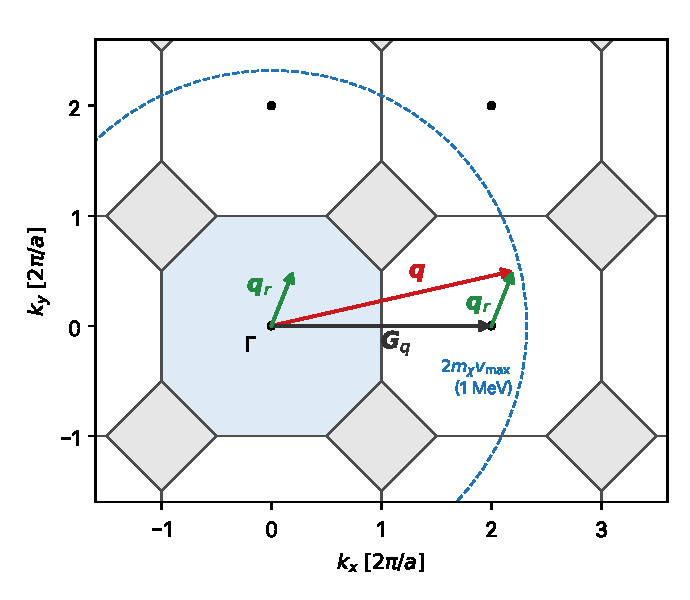
\includegraphics[width=0.62\linewidth]{figures/ch03/fig3_3.pdf}
  \caption{A momentum transfer reduced to the first Brillouin zone, in the plane $k_z = 0$ of the fcc reciprocal lattice, with momenta in units of $2\pi/a$ (\SI{2.28}{keV} for silicon). Dots: the reciprocal-lattice vectors in this plane, $(2\pi/a)(2m,2n,0)$. Octagons: the cuts of their Brillouin zones by the plane; the first zone is shaded blue. The grey squares belong to zones centered on reciprocal-lattice vectors $(2\pi/a)(h,k,\pm1)$ with $h, k$ odd, which lie outside the plane. The momentum transfer $\vect{q} = (2\pi/a)(2.2, 0.5, 0)$, of length \SI{5.15}{keV}, is the sum of the reciprocal-lattice vector $\vect{G}_q = (2\pi/a)(2,0,0)$ nearest to it and of $\vect{q}_r = (2\pi/a)(0.2, 0.5, 0)$, of length \SI{1.23}{keV}, drawn both at $\vect{G}_q$ and at the origin. Dashed circle: the maximum momentum transfer $2\mchi v_{\mathrm{max}} = \SI{5.30}{keV}$ of dark matter of mass \SI{1}{MeV}, with $v_{\mathrm{max}} = \SI{794.5}{km.s^{-1}}$.}
  \label{fig:3-umklapp}
\end{figure}

The momentum transfer itself is never reduced to the first zone. The dark matter loses $\vect{q}$, not $\vect{q}_r$, and its kinematics, $\vmin$ and the dark-matter form factor $\FDM(q)$ (\cref{sec:1.3,sec:1.4}) depend on $|\vect{q}|$. The target does not treat $\vect{q}$ and $\vect{q}_r$ alike either. Both change the crystal momentum by the same amount. However, the plane wave $\ee^{\ii\vect{q}\cdot\vect{r}}$ varies on the scale $2\pi/|\vect{q}|$ and resolves the electron density inside the cell on that scale. At large $|\vect{G}_q|$ it probes the region near the nuclei, where the core electrons and the steep part of the valence wavefunctions sit (\cref{sec:3.5}). The response of the crystal is therefore a function of $\vect{q}_r$ and $\vect{G}_q$ separately, not of $\vect{q}_r$ alone, and the book keeps both (\cref{app:A.3}).

\begin{workedexample}{Momentum transfers against the zone of silicon}\label{we:3-scales}
With $\hbar c = \SI{1973.27}{eV.\angstrom}$ and $a = \SI{5.431}{\angstrom}$,
\begin{equation*}
  \frac{2\pi}{a} = \frac{2\pi \times \SI{1973.27}{eV.\angstrom}}{\SI{5.431}{\angstrom}} = \SI{2283}{eV} = \SI{2.28}{keV} .
\end{equation*}
The shortest reciprocal-lattice vectors are $|\vect{G}_{111}| = \SI{3.95}{keV}$ and $|\vect{G}_{200}| = \SI{4.57}{keV}$. An electronic excitation across the low-temperature gap, $\Eg = \SI{1.17}{eV}$ (\cref{sec:3.3}), needs $q \ge \Eg/v_{\mathrm{max}} = \SI{1.17}{eV}/(2.650\times10^{-3}) = \SI{0.44}{keV}$, or $0.19\,(2\pi/a)$, deep inside the zone. The largest momentum transfer that can still deposit $\Eg$ follows from \cref{eq:1.3-region}, $q = \mchi v_{\mathrm{max}}[1 + (1 - 2\Eg/\mchi v_{\mathrm{max}}^2)^{1/2}]$. It is \SI{4.81}{keV} $= 2.11\,(2\pi/a)$ for $\mchi = \SI{1}{MeV}$, \SI{52.6}{keV} $= 23.0\,(2\pi/a)$ for \SI{10}{MeV} and \SI{530}{keV} $= 232\,(2\pi/a)$ for \SI{100}{MeV}. The lower end of the range is \SI{0.49}{keV} at \SI{1}{MeV} and tends to $\Eg/v_{\mathrm{max}} = \SI{0.44}{keV}$ for heavier particles, hardly depending on the mass; the upper end grows in proportion to $\mchi$.

Already at \SI{1}{MeV} the range extends past the eight $\vect{G}_{111}$ and the six $\vect{G}_{200}$, and the typical momentum of a valence electron, $q_0 = \SI{3.73}{keV} = 1.63\,(2\pi/a)$, lies outside the zone. A ball of radius $q$ contains about $(4\pi/3)q^3/[4(2\pi/a)^3]$ reciprocal-lattice vectors, one per zone volume. For the maximum momentum transfer $2\mchi v_{\mathrm{max}}$ this is $\num{1.3e4}$ at \SI{10}{MeV}, which a direct count confirms, and $\num{1.3e7}$ at \SI{100}{MeV}. Above about a MeV, most of the kinematically allowed momentum transfers have $\vect{G}_q \neq 0$, and a calculation of the rate must carry the response out to reciprocal-lattice vectors whose number grows as $\mchi^3$ (\cref{sec:3.5,app:E.7}).
\end{workedexample}

\subsection{The basis structure factor}

The positions of the atoms within the cell enter every Fourier component of a lattice-periodic quantity. Consider a function built from one term per atom, $f(\vect{r}) = \sum_{\vect{R}}\sum_\kappa v_\kappa(\vect{r} - \vect{R} - \vect{\tau}_\kappa)$, such as the potential of the clamped nuclei or a superposition of atomic charge densities. Its components, \cref{eq:A.3-periodic}, are
\begin{equation*}
  f_{\vect{G}} = \frac{1}{\Omega}\int_\Omega\dd^3r\;\ee^{\ii\vect{G}\cdot\vect{r}}\sum_{\vect{R}}\sum_\kappa v_\kappa(\vect{r} - \vect{R} - \vect{\tau}_\kappa)
  = \frac{1}{\Omega}\sum_\kappa\int\dd^3r\;\ee^{\ii\vect{G}\cdot\vect{r}}\,v_\kappa(\vect{r} - \vect{\tau}_\kappa) .
\end{equation*}
In the second step, the translate of the cell by $-\vect{R}$ was used for each term; since $\ee^{\ii\vect{G}\cdot\vect{R}} = 1$, the phase is unchanged, and the cells together fill all of space. Shifting $\vect{r}$ by $\vect{\tau}_\kappa$ then gives
\begin{equation}
  f_{\vect{G}} = \frac{1}{\Omega}\sum_\kappa\ee^{\ii\vect{G}\cdot\vect{\tau}_\kappa}\,\tilde v_\kappa(\vect{G}),
  \qquad \tilde v_\kappa(\vect{G}) = \int\dd^3x\;\ee^{\ii\vect{G}\cdot\vect{x}}\,v_\kappa(\vect{x}) .
  \label{eq:3.1-fG}
\end{equation}
Each atom contributes the transform of its own term at $\vect{G}$, with a phase set by its position in the cell. When all atoms of the basis are of one element, $\tilde v_\kappa = \tilde v$, the positions factor out into the \emph{basis structure factor}
\begin{equation}
  S^{\mathrm{bas}}(\vect{G}) = \sum_\kappa\ee^{\ii\vect{G}\cdot\vect{\tau}_\kappa},
  \label{eq:3.1-Sbas}
\end{equation}
and $f_{\vect{G}} = S^{\mathrm{bas}}(\vect{G})\,\tilde v(\vect{G})/\Omega$. A zero of $S^{\mathrm{bas}}$ is an \emph{extinction}: the component vanishes at that reciprocal-lattice vector, whatever the atomic term, because the contributions of the atoms in the cell cancel.

The nuclei of \cref{sec:2.3} are the simplest case. Their density for site $\kappa$, $n_\kappa(\vect{k}) = \sum_{\vect{R}}\ee^{\ii\vect{k}\cdot(\vect{R} + \vect{\tau}_\kappa)}$, becomes with \cref{eq:3.1-latticesum}
\begin{equation*}
  \sum_\kappa Z_\kappa\,n_\kappa(\vect{k}) = N\sum_{\vect{G}}\delta_{\vect{k},\vect{G}}\sum_\kappa Z_\kappa\,\ee^{\ii\vect{G}\cdot\vect{\tau}_\kappa} ,
\end{equation*}
nonzero only at reciprocal-lattice vectors, as \cref{sec:2.3} anticipated. The electron--nucleus potential of \cref{eq:2.3-HC} then has the components of \cref{eq:3.1-fG} with $\tilde v_\kappa(\vect{G}) = -Z_\kappa v_{\mathrm{C}}(|\vect{G}|)$. The same expression describes dark matter that couples to the clamped nuclei: it can transfer only a reciprocal-lattice vector, elastically, with no energy deposited. This is the coherent, Bragg-like part of the response mentioned in \cref{sec:2.2}, and a static lattice has no other nuclear response. Energy reaches the nuclei once they are allowed to move (\cref{chap:5}).

\begin{workedexample}{The diamond structure factor and the absent (200) reflection}\label{we:3-diamond}
For $\vect{G} = (2\pi/a)(h,k,l)$ and the basis of \cref{eq:3.1-basis}, $\vect{G}\cdot\vect{\tau}_2 = (\pi/2)(h + k + l)$, and \cref{eq:3.1-Sbas} gives
\begin{equation*}
  S^{\mathrm{bas}}(\vect{G}_{hkl}) = 1 + \ee^{\ii\pi(h + k + l)/2} .
\end{equation*}
For $h, k, l$ all odd, $h + k + l$ is odd and $S^{\mathrm{bas}} = 1 \pm \ii$, with $|S^{\mathrm{bas}}|^2 = 2$; for (111), $h + k + l = 3$ and $S^{\mathrm{bas}} = 1 - \ii$. For $h, k, l$ all even, $h + k + l$ is even, and two cases arise. If $h + k + l$ is a multiple of four, as for (220) and (400), the two atoms add in phase, $S^{\mathrm{bas}} = 2$ and $|S^{\mathrm{bas}}|^2 = 4$. If $h + k + l = 4n + 2$, as for (200) and (222), $S^{\mathrm{bas}} = 1 + \ee^{\ii\pi} = 0$. The plane wave at $\vect{G}_{200}$ has its crests on the atoms at $\vect{\tau}_1$ and its troughs on those at $\vect{\tau}_2$, a quarter cube diagonal away, and the two contributions cancel.

The (200) and (222) reflections of silicon are therefore absent in X-ray diffraction from spherical atoms, although $\vect{G}_{200}$ and $\vect{G}_{222}$ are reciprocal-lattice vectors of its fcc lattice and $\vect{G}_{200}$ is the second-shortest. The same cancellation removes these components from any part of the crystal potential that is a sum of identical spherical atomic terms. The (222) component returns through the part of the potential that is not of this form, such as the charge that piles up in the bonds (\cref{sec:3.4}), and is observed as a weak X-ray reflection. The (200) component does not. The diamond structure is mapped onto itself by \emph{glides}, each a reflection in a plane parallel to a cube face followed by a translation by a quarter of a face diagonal within that plane. The glides force it to vanish for every function with the symmetry of the crystal (\cref{app:C.17}). In zincblende GaAs the two sites hold different nuclei, $Z_\kappa = 31$ (gallium) and 33 (arsenic), and the nuclear factor $\sum_\kappa Z_\kappa\ee^{\ii\vect{G}\cdot\vect{\tau}_\kappa}$ equals $31 - 33 = -2$ at (200), against $31 + 33 = 64$ at (220). The (200) component is weak, smaller in square by a factor of $4/4096 \approx 10^{-3}$, but not zero, and it is what distinguishes the zincblende structure from diamond in diffraction.
\end{workedexample}

Extinctions also explain why the fcc reciprocal lattice lacks the vectors $(2\pi/a)(h,k,l)$ of mixed parity. The fcc lattice can also be described as a simple cubic lattice of side $a$ with a basis of four points, at a corner and the three adjacent face centers. Its reciprocal lattice is then simple cubic, $(2\pi/a)(h,k,l)$ with any integers, and the structure factor of the four points is $1 + \ee^{\ii\pi(h + k)} + \ee^{\ii\pi(k + l)} + \ee^{\ii\pi(l + h)}$, which is 4 when $h, k, l$ have one parity and 0 otherwise. A basis structure factor is the price of using a cell larger than the primitive one, and its zeros remove exactly the vectors that the smaller cell does not have.

The electrons move in the periodic potential whose components \cref{eq:3.1-fG} describes. \Cref{sec:3.2} shows that their states are labeled by a crystal momentum in the zone and a band index, and computes the matrix element of $\ee^{\ii\vect{q}\cdot\vect{r}}$ between them, with the Umklapp vector kept in the plane wave.

\section{Bloch states and band structure}\label{sec:3.2}

An electron in silicon moves in a potential that repeats itself after every lattice vector: the attraction of the clamped nuclei, the repulsion of the other electrons, and the exchange and correlation effects that come with them (\cref{sec:2.3}). The full problem is a many-electron one. Most of what a dark-matter rate needs, however, can be understood with each electron moving independently in an effective potential $U(\vect{r})$ with the periodicity of the lattice, $U(\vect{r} + \vect{R}) = U(\vect{r})$. Density-functional theory supplies the best such potential and tells us what it leaves out (\cref{sec:3.4}). Here $U$ is any lattice-periodic function, and its periodicity alone fixes the form of the states and the momentum transfers that connect them. Bands and gaps are understood in two opposite limits, nearly free electrons and tight binding. We then compute the two matrix elements that every electronic rate in this book contains: that of $\ee^{\ii\vect{q}\cdot\vect{r}}$, to which dark matter couples, and that of the velocity, to which light couples. We follow Refs.~\cite[Chaps.~8--10]{ashcroft1976solid}, \cite[Chap.~3]{harrison1980electronic} and \cite[Chap.~2]{yu2010fundamentals}.

\subsection{Bloch's theorem}

The one-electron Hamiltonian is
\begin{equation}
  H_{\mathrm{e}} = \frac{\op{\vect{p}}^2}{2m_e} + U(\vect{r}), \qquad U(\vect{r} + \vect{R}) = U(\vect{r}) ,
  \label{eq:3.2-He}
\end{equation}
with $\op{\vect{p}} = -\ii\nabla$. We keep the electron spinless and count the two spin states with an explicit factor of 2; spin--orbit coupling, which mixes them, enters in \cref{sec:3.3}. The translation operator of \cref{sec:3.1}, acting now on one electron, is $(T_{\vect{R}}\psi)(\vect{r}) = \psi(\vect{r} + \vect{R})$. The kinetic energy is unchanged by any translation, and $U$ by a lattice translation, so every $T_{\vect{R}}$ commutes with $H_{\mathrm{e}}$. The argument that led to \cref{eq:3.1-crystalmomentum} then applies to a single electron: the eigenstates of $H_{\mathrm{e}}$ can be chosen so that $\psi(\vect{r} + \vect{R}) = \ee^{\ii\vect{k}\cdot\vect{R}}\psi(\vect{r})$ for every $\vect{R}$, with $\vect{k}$ in the first Brillouin zone and on the Born--von Karman grid of \cref{eq:3.1-kgrid}. Define $u(\vect{r}) = \ee^{-\ii\vect{k}\cdot\vect{r}}\psi(\vect{r})$. It is periodic, since $u(\vect{r} + \vect{R}) = \ee^{-\ii\vect{k}\cdot\vect{r}}\ee^{-\ii\vect{k}\cdot\vect{R}}\,\ee^{\ii\vect{k}\cdot\vect{R}}\psi(\vect{r}) = u(\vect{r})$. Each eigenstate is therefore a plane wave modulated by a function with the period of the lattice:
\begin{keyresult}[Bloch's theorem]
\begin{equation}
  \psi_{n\vect{k}}(\vect{r}) = \frac{1}{\sqrt N}\,\ee^{\ii\vect{k}\cdot\vect{r}}\,u_{n\vect{k}}(\vect{r}), \qquad
  u_{n\vect{k}}(\vect{r} + \vect{R}) = u_{n\vect{k}}(\vect{r}), \qquad
  \int_\Omega\dd^3r\,|u_{n\vect{k}}|^2 = 1 .
  \label{eq:3.2-bloch}
\end{equation}
Equivalently, $\psi_{n\vect{k}}(\vect{r} + \vect{R}) = \ee^{\ii\vect{k}\cdot\vect{R}}\psi_{n\vect{k}}(\vect{r})$. The state is normalized to one over the crystal of volume $\Vol = N\Omega$, and its periodic part to one over a cell.
\end{keyresult}
The two normalizations agree because $|\psi_{n\vect{k}}|^2 = |u_{n\vect{k}}|^2/N$ is periodic and the crystal holds $N$ cells; these are the conventions of \cref{app:A.5}. The label $n$, the \emph{band index}, appears because there are many solutions at each $\vect{k}$. Inserting $\psi = N^{-1/2}\ee^{\ii\vect{k}\cdot\vect{r}}u$ into $H_{\mathrm{e}}\psi = \varepsilon\psi$ and using $\op{\vect{p}}\,\ee^{\ii\vect{k}\cdot\vect{r}}u = \ee^{\ii\vect{k}\cdot\vect{r}}(\op{\vect{p}} + \vect{k})u$ leaves an equation for $u$ alone,
\begin{equation}
  H_{\vect{k}}\,u_{n\vect{k}} = \varepsilon_{n\vect{k}}\,u_{n\vect{k}}, \qquad
  H_{\vect{k}} \equiv \ee^{-\ii\vect{k}\cdot\vect{r}}H_{\mathrm{e}}\,\ee^{\ii\vect{k}\cdot\vect{r}} = \frac{(\op{\vect{p}} + \vect{k})^2}{2m_e} + U(\vect{r}) ,
  \label{eq:3.2-Hk}
\end{equation}
to be solved in one cell with periodic boundary conditions. Like a particle in a box, $H_{\vect{k}}$ has a discrete spectrum at each $\vect{k}$, which we order as $\varepsilon_{1\vect{k}} \le \varepsilon_{2\vect{k}} \le \dots$. Since $\vect{k}$ enters $H_{\vect{k}}$ as a parameter, each \emph{band energy} $\varepsilon_{n\vect{k}}$ varies continuously with $\vect{k}$ and sweeps out an energy band; the set of all of them, plotted along lines through the zone, is the \emph{band structure}. The bands are periodic in reciprocal space: $\ee^{-\ii\vect{G}\cdot\vect{r}}u_{n\vect{k}}$ is periodic and satisfies $H_{\vect{k}+\vect{G}}\,\ee^{-\ii\vect{G}\cdot\vect{r}}u_{n\vect{k}} = \ee^{-\ii\vect{G}\cdot\vect{r}}H_{\vect{k}}u_{n\vect{k}}$, so $\varepsilon_{n,\vect{k}+\vect{G}} = \varepsilon_{n\vect{k}}$. We use this freedom to identify the states themselves, $\psi_{n,\vect{k}+\vect{G}} = \psi_{n\vect{k}}$, which is the \emph{periodic gauge} of \cref{eq:A.5-periodic}. A crystal momentum outside the first zone can then be used directly.

A Bloch state is not a state of definite momentum. Its periodic part is a Fourier series over reciprocal-lattice vectors, and we write it in the convention of plane-wave codes (\cref{app:A.3}),
\begin{equation}
  u_{n\vect{k}}(\vect{r}) = \frac{1}{\sqrt\Omega}\sum_{\vect{G}}c_{n\vect{k}}(\vect{G})\,\ee^{\ii\vect{G}\cdot\vect{r}}, \qquad
  \psi_{n\vect{k}}(\vect{r}) = \frac{1}{\sqrt \Vol}\sum_{\vect{G}}c_{n\vect{k}}(\vect{G})\,\ee^{\ii(\vect{k}+\vect{G})\cdot\vect{r}}, \qquad
  \sum_{\vect{G}}|c_{n\vect{k}}(\vect{G})|^2 = 1 .
  \label{eq:3.2-pw}
\end{equation}
The coefficient $c_{n\vect{k}}(\vect{G})$ multiplies $\ee^{+\ii\vect{G}\cdot\vect{r}}$, so it is the lattice Fourier component of \cref{eq:A.3-periodic} at $-\vect{G}$, times $\Omega^{1/2}$. The electron in state $n\vect{k}$ has the momenta $\vect{k} + \vect{G}$, with probabilities $|c_{n\vect{k}}(\vect{G})|^2$. A smooth valence state is dominated by a few small $\vect{G}$; the part of the wavefunction near the nuclei, where it oscillates rapidly, puts weight at large $|\vect{G}|$, and it is this tail that a momentum transfer of many keV probes (\cref{sec:3.5}).

The same expansion turns \cref{eq:3.2-Hk} into an algebraic equation and provides a second proof of Bloch's theorem. Write the potential as $U(\vect{r}) = \sum_{\vect{G}''}U_{\vect{G}''}\,\ee^{-\ii\vect{G}''\cdot\vect{r}}$, with the components $U_{\vect{G}} = \Omega^{-1}\int_\Omega\dd^3r\,\ee^{\ii\vect{G}\cdot\vect{r}}U(\vect{r})$ of \cref{eq:A.3-periodic}. Acting on a plane wave, $U$ produces $U(\vect{r})\,\ee^{\ii(\vect{k}+\vect{G}')\cdot\vect{r}} = \sum_{\vect{G}''}U_{\vect{G}''}\,\ee^{\ii(\vect{k}+\vect{G}'-\vect{G}'')\cdot\vect{r}}$. Collecting the coefficient of $\ee^{\ii(\vect{k}+\vect{G})\cdot\vect{r}}$ in $H_{\mathrm{e}}\psi_{n\vect{k}} = \varepsilon_{n\vect{k}}\psi_{n\vect{k}}$ picks the term $\vect{G}'' = \vect{G}' - \vect{G}$, and
\begin{equation}
  \Bigl[\frac{(\vect{k} + \vect{G})^2}{2m_e} - \varepsilon_{n\vect{k}}\Bigr]c_{n\vect{k}}(\vect{G}) + \sum_{\vect{G}'}U_{\vect{G}'-\vect{G}}\,c_{n\vect{k}}(\vect{G}') = 0 .
  \label{eq:3.2-central}
\end{equation}
A periodic potential couples a plane wave only to those that differ from it by a reciprocal-lattice vector. A state built from one $\vect{k}$ and its translates $\vect{k} + \vect{G}$ stays among them, which is Bloch's theorem again. The matrix $(\vect{k}+\vect{G})^2\delta_{\vect{G}\vect{G}'}/2m_e + U_{\vect{G}'-\vect{G}}$ is Hermitian, since a real $U$ has $U_{-\vect{G}} = U^*_{\vect{G}}$. Its eigenvalues are the $\varepsilon_{n\vect{k}}$, and its eigenvectors the $c_{n\vect{k}}(\vect{G})$. A plane-wave code diagonalizes this matrix, truncated at a cutoff in $|\vect{k}+\vect{G}|$ (\cref{sec:3.5}).

Bloch states with different $\vect{k}$ are orthogonal, because they belong to different eigenvalues of the unitary $T_{\vect{R}}$, and states with the same $\vect{k}$ and different $n$ are orthogonal as eigenvectors of the Hermitian $H_{\vect{k}}$. Together they form an orthonormal basis, and the change of basis of \cref{eq:2.3-basis} turns the plane-wave operators of \cref{sec:2.3} into operators $c^\dagger_{n\vect{k}s}$ and $c_{n\vect{k}s}$ that create and destroy an electron of spin $s$ in a Bloch state. For independent electrons the Hamiltonian is $\sum_{n\vect{k}s}\varepsilon_{n\vect{k}}\,c^\dagger_{n\vect{k}s}c_{n\vect{k}s}$, and in thermal equilibrium the \emph{occupation} of a state is, by \cref{eq:2.5-nF},
\begin{equation}
  f_{n\vect{k}} = \langle c^\dagger_{n\vect{k}s}c_{n\vect{k}s}\rangle = n_{\mathrm{F}}(\varepsilon_{n\vect{k}} - \mu_{\mathrm{ch}}) .
  \label{eq:3.2-fnk}
\end{equation}
Each band holds $2N$ electrons, as \cref{sec:3.1} counted. In silicon the eight valence electrons per cell fill the four lowest bands, and a gap of about an electronvolt separates them from the next ones (\cref{sec:3.3}). At any temperature at which a detector runs, $f_{n\vect{k}} = 1$ in these four bands and $0$ above them, to an accuracy set by $\ee^{-\Eg/2T}$, the factor that the intrinsic carrier density of \cref{eq:3.3-ni} carries. Two questions follow: where such gaps come from, and how $\ee^{\ii\vect{q}\cdot\vect{r}}$ connects the states on either side of them.

\subsection{Nearly free electrons}

Switch the potential off. The eigenstates of \cref{eq:3.2-central} are then single plane waves, $c_{n\vect{k}}(\vect{G}) = \delta_{\vect{G},\vect{G}_n}$ for some vector $\vect{G}_n$ that labels the band, with energies $\varepsilon^0_{\vect{k}+\vect{G}_n}$. Here $\varepsilon^0_{\vect{k}} = k^2/2m_e$ is the free-electron energy at wavevector $\vect{k}$, inside the zone or not. Nothing physical has changed: the free parabola has been cut into pieces and each piece shifted by a reciprocal-lattice vector into the first zone, so that at a given $\vect{k}$ the bands are the parabolas centered on all the $-\vect{G}$. This is the \emph{empty-lattice} band structure, drawn dashed in \cref{fig:3-nfe}(a). Its bands cross wherever two plane waves have equal energy, $\varepsilon^0_{\vect{k}} = \varepsilon^0_{\vect{k}-\vect{G}}$, that is, on the planes $\vect{k}\cdot\vect{G} = |\vect{G}|^2/2$ that bisect the reciprocal-lattice vectors. These are the Bragg planes whose pieces bound the Brillouin zone (\cref{sec:3.1}).

Now let $U$ be weak. Away from a crossing, the coupling $U_{\vect{G}'-\vect{G}}$ mixes plane waves whose energies differ by much more than $|U|$, and second-order perturbation theory shifts each level by $\sum_{\vect{G}\neq0}|U_{\vect{G}}|^2/(\varepsilon^0_{\vect{k}} - \varepsilon^0_{\vect{k}-\vect{G}})$, a small correction. Near a crossing, however, two plane waves are degenerate and perturbation theory in this form fails. We keep just those two, $\ee^{\ii\vect{k}\cdot\vect{r}}$ and $\ee^{\ii(\vect{k}-\vect{G})\cdot\vect{r}}$. \Cref{eq:3.2-central} for the coefficients $c(0)$ and $c(-\vect{G})$ reads
\begin{equation}
  \begin{pmatrix} \varepsilon^0_{\vect{k}} & U_{-\vect{G}} \\ U_{\vect{G}} & \varepsilon^0_{\vect{k}-\vect{G}} \end{pmatrix}
  \begin{pmatrix} c(0) \\ c(-\vect{G}) \end{pmatrix} = \varepsilon \begin{pmatrix} c(0) \\ c(-\vect{G}) \end{pmatrix},
  \label{eq:3.2-twowave}
\end{equation}
where the diagonal $U_0$, a constant shift, has been absorbed into the energy zero. The eigenvalues are
\begin{equation}
  \varepsilon_\pm = \frac{\varepsilon^0_{\vect{k}} + \varepsilon^0_{\vect{k}-\vect{G}}}{2} \pm \sqrt{\Bigl(\frac{\varepsilon^0_{\vect{k}} - \varepsilon^0_{\vect{k}-\vect{G}}}{2}\Bigr)^2 + |U_{\vect{G}}|^2} .
  \label{eq:3.2-epm}
\end{equation}
Far from the plane the square root tends to $|\varepsilon^0_{\vect{k}} - \varepsilon^0_{\vect{k}-\vect{G}}|/2$, and the two free parabolas are recovered. On the plane the two free energies are equal, and the levels are pushed apart symmetrically:
\begin{keyresult}[Nearly-free-electron gap]
On the Bragg plane $\vect{k}\cdot\vect{G} = |\vect{G}|^2/2$, a weak periodic potential splits the two degenerate plane waves into $\varepsilon_\pm = \varepsilon^0_{\vect{k}} \pm |U_{\vect{G}}|$. The gap,
\begin{equation}
  \varepsilon_+ - \varepsilon_- = 2|U_{\vect{G}}| ,
  \label{eq:3.2-gap}
\end{equation}
is set by the Fourier component of the potential at the reciprocal-lattice vector that the plane bisects. It holds to first order in $U$, as long as $|U_{\vect{G}}|$ is small compared with the energy separation to the next plane waves.
\end{keyresult}
At the zone boundary the band structure therefore has a gap, and no state of the crystal has an energy inside it, whatever the direction of $\vect{k}$ along the plane. Whether the gaps on different faces of the zone overlap in energy and leave a gap for the whole crystal depends on the sizes of the $U_{\vect{G}}$ and on the shape of the zone. In a nearly-free metal such as aluminium they do not, and a Fermi surface survives~\cite[Chap.~9]{ashcroft1976solid}. Note that a component that vanishes by extinction (\cref{we:3-diamond}) opens no gap at first order. In silicon, the square faces of the zone bisect $\vect{G}_{200}$, and $U_{\vect{G}_{200}} = 0$ exactly, by the glide symmetry of the diamond structure (\cref{we:3-diamond}, \cref{app:C.17}).

The states at the gap are standing waves. For a potential with inversion symmetry and real $U_{\vect{G}} = U_{-\vect{G}}$, the eigenvectors of \cref{eq:3.2-twowave} on the plane are $c(-\vect{G}) = \pm c(0)$, so that $\psi \propto \ee^{\ii\vect{G}\cdot\vect{r}/2} \pm \ee^{-\ii\vect{G}\cdot\vect{r}/2}$ for $\vect{k} = \vect{G}/2$: a cosine and a sine of $\vect{G}\cdot\vect{r}/2$. The two have the same kinetic energy, but the cosine piles the electron density up at the points where $\vect{G}\cdot\vect{r}$ is a multiple of $2\pi$, the lattice planes, and the sine piles it up halfway between them. If the potential is attractive at the planes, $U_{\vect{G}} < 0$, the cosine lies lower by $|U_{\vect{G}}|$ and the sine higher by the same amount. A running wave at the boundary would be Bragg-reflected into its partner at $\vect{k} - \vect{G}$; the two standing waves are what remains, and both carry no current. The group velocity, the slope of the band (\cref{eq:3.2-vg} below), vanishes on the Bragg plane in the direction of $\vect{G}$, and the bands meet the zone boundary with zero slope, as \cref{fig:3-nfe}(a) shows.

\begin{figure}[tbp]
  \centering
  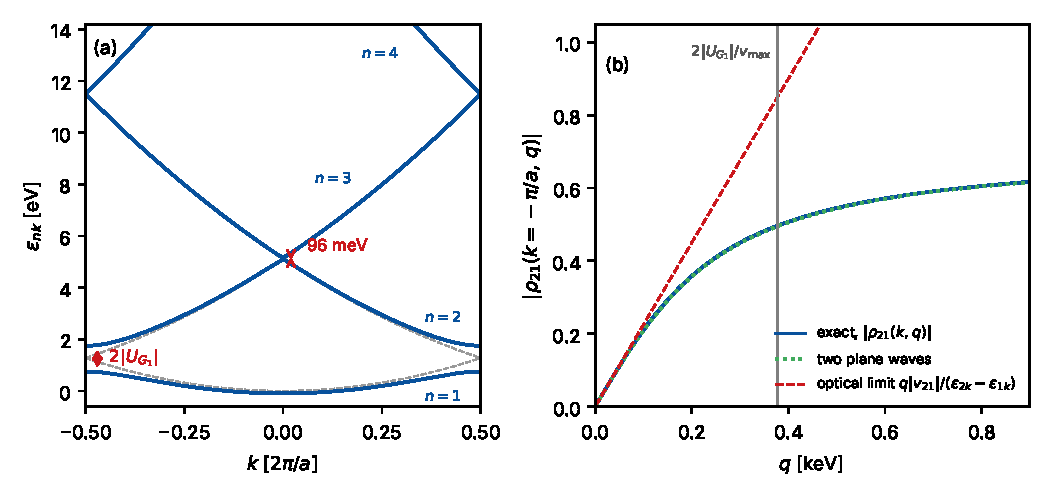
\includegraphics[width=\linewidth]{figures/ch03/fig3_4.pdf}
  \caption{Nearly free electrons in one dimension, for the potential $U(x) = 2U_{G_1}\cos(G_1x)$ with $G_1 = 2\pi/a$, $a = \SI{5.431}{\angstrom}$ (the lattice constant of silicon, used only to set the scale) and $U_{G_1} = \SI{-0.5}{eV}$. The bands are computed by diagonalizing \cref{eq:3.2-central} in 25 plane waves $\ee^{\ii(k+jG_1)x}$, $|j| \le 12$. (a)~The four lowest bands $\varepsilon_{nk}$ (solid) and the free-electron parabolas $(k + jG_1)^2/2m_e$ folded into the first zone (dashed). The first gap, at the zone boundary $k = \pm\pi/a$, is \SI{0.998}{eV}, close to $2|U_{G_1}| = \SI{1}{eV}$; the second, at $k = 0$, is \SI{96}{meV}, second order in $U_{G_1}$, since the potential has no component at $2G_1$. (b)~The density vertex $|\rho_{21}(k, q)|$ between the two lowest bands at $k = -\pi/a$, for momentum transfers $0 < q < \SI{0.9}{keV}$, which keep $k + q$ in the first zone. Solid: the full calculation. Dotted: the two-plane-wave model, indistinguishable at this scale. Dashed: the optical limit $q|v_{21}(k)|/(\varepsilon_{2k} - \varepsilon_{1k})$. The vertical line marks the smallest momentum transfer at which dark matter can deposit \SI{1}{eV}, $2|U_{G_1}|/v_{\mathrm{max}} = \SI{0.38}{keV}$ for $v_{\mathrm{max}} = 2.650\times10^{-3}$.}
  \label{fig:3-nfe}
\end{figure}

\begin{workedexample}{The one-dimensional gap}\label{we:3-gap1d}
Take the one-dimensional potential $U(x) = 2U_{G_1}\cos(G_1x)$, whose only components are $U_{\pm G_1} = U_{G_1}$, with $U_{G_1} = \SI{-0.5}{eV}$ and the period $a = \SI{5.431}{\angstrom}$, so that $G_1 = 2\pi/a = \SI{2283}{eV}$. The potential is attractive at the lattice sites, $U(0) = \SI{-1}{eV}$. The free-electron energy at the zone boundary, $k = G_1/2$, is
\begin{equation*}
  \varepsilon^0_{G_1/2} = \frac{(G_1/2)^2}{2m_e} = \frac{(\SI{1141.5}{eV})^2}{2\times\SI{511.0}{keV}} = \SI{1.275}{eV} ,
\end{equation*}
and \cref{eq:3.2-epm} puts the band edges at $\SI{1.275}{eV} \mp \SI{0.5}{eV}$, that is, at 0.775 and \SI{1.775}{eV}, with the gap $2|U_{G_1}| = \SI{1.000}{eV}$. The lower edge is the cosine, concentrated on the sites, and the upper edge the sine, concentrated between them; the full calculation of \cref{fig:3-nfe} confirms that $|\psi|^2$ of the lower state vanishes at $x = a/2$, and that of the upper state at $x = 0$.

Diagonalizing \cref{eq:3.2-central} in 25 plane waves gives the edges 0.752 and \SI{1.749}{eV}, and the gap \SI{0.998}{eV}. The lower edge has moved down by \SI{0.023}{eV} and the upper by \SI{0.026}{eV}. The shift comes from the next plane waves, $\ee^{\ii(G_1/2 + G_1)x}$ and $\ee^{\ii(-G_1/2 - G_1)x}$, which each of the two boundary states can reach with one factor of $U_{G_1}$. Their energy is $9\times\SI{1.275}{eV} = \SI{11.47}{eV}$, and second-order perturbation theory yields $U_{G_1}^2/(\SI{1.275}{eV} - \SI{11.47}{eV}) = \SI{-0.025}{eV}$ for each edge, the average of the two computed shifts. The gap $2|U_{G_1}|$ is thus accurate to \SI{0.2}{\percent}, although $|U_{G_1}|$ is \SI{40}{\percent} of the kinetic energy at the boundary.

The second gap is a different matter. It opens at $k = 0$, where the plane waves $\ee^{\pm\ii G_1x}$ are degenerate at $\varepsilon^0_{G_1} = \SI{5.099}{eV}$. They differ by $2G_1$, and $U_{2G_1} = 0$, so they are not coupled directly. They are coupled at second order through the plane wave $\ee^{\ii0x}$, with the effective matrix element $U_{G_1}^2/(\varepsilon^0_{G_1} - \varepsilon^0_0) = \SI{0.049}{eV}$, and the two-level splitting is twice this, \SI{0.098}{eV}. The full calculation finds \SI{0.096}{eV}. A gap at a Bragg plane is first order in the component of $U$ at that $\vect{G}$, and higher order if that component vanishes. This is what happens on the square faces of the silicon zone, where the extinction of $\vect{G}_{200}$ removes the first-order term.
\end{workedexample}

Silicon is not in the regime where these estimates are quantitative. A three-dimensional gap requires the gaps on all faces of the zone to overlap in energy, and in silicon the band edges lie at different crystal momenta (\cref{sec:3.3}). Its potential is not weak either: the free-electron energy at $\mathrm{L}$ is $|\vect{G}_{111}|^2/8m_e = \SI{3.82}{eV}$, and the strong attraction of the ion cores mixes many plane waves into each state, a problem that the pseudopotentials of \cref{sec:3.5} remove. What survives is the mechanism. Gaps open where the free-electron energy surfaces cross the Bragg planes, and they are set by the Fourier components of the potential. The opposite limit, in which electrons hop between atomic orbitals, explains why silicon has a gap where it does.

\subsection{Tight binding and the \texorpdfstring{$sp^3$}{sp3} bond}

A silicon atom in the gas has two $3s$ and two $3p$ electrons in sharp atomic levels. Bring the atoms together into a crystal of $N$ cells, and each atomic level of each atom in the cell broadens into a band of $N$ states, because the electrons can now hop from atom to atom. When the hopping is weak compared with the spacing of the atomic levels, the natural starting point is the atomic orbitals, not plane waves. This is the \emph{tight-binding} method, or the linear combination of atomic orbitals (LCAO).

Let $\varphi^{\mathrm{at}}_j(\vect{r})$ be atomic orbitals, with $j$ labeling both the orbital and the site $\vect{\tau}_\kappa$ of the basis on which it is centered, and $\varphi^{\mathrm{at}}_{j\vect{R}}(\vect{r}) = \varphi^{\mathrm{at}}_j(\vect{r} - \vect{R})$ its copy in cell $\vect{R}$. No single orbital has the form \cref{eq:3.2-bloch}, but the \emph{Bloch sum}
\begin{equation}
  |j\vect{k}\rangle = \frac{1}{\sqrt N}\sum_{\vect{R}}\ee^{\ii\vect{k}\cdot\vect{R}}\,|\varphi^{\mathrm{at}}_{j\vect{R}}\rangle ,
  \label{eq:3.2-blochsum}
\end{equation}
does: translating it by a lattice vector $\vect{R}'$ relabels the sum and multiplies it by $\ee^{\ii\vect{k}\cdot\vect{R}'}$. Since $H_{\mathrm{e}}$ commutes with lattice translations, it does not connect Bloch sums of different $\vect{k}$, and we look for the states as $|\psi_{n\vect{k}}\rangle = \sum_jC_{nj}(\vect{k})\,|j\vect{k}\rangle$, with one coefficient per orbital in the cell. The matrix elements between Bloch sums reduce to sums over one lattice vector. Translation invariance gives $\langle\varphi^{\mathrm{at}}_{j\vect{R}}|H_{\mathrm{e}}|\varphi^{\mathrm{at}}_{j'\vect{R}'}\rangle = \langle\varphi^{\mathrm{at}}_{j\vect{0}}|H_{\mathrm{e}}|\varphi^{\mathrm{at}}_{j',\vect{R}'-\vect{R}}\rangle$. The double sum over $\vect{R}$ and $\vect{R}'$ in $\langle j\vect{k}|H_{\mathrm{e}}|j'\vect{k}\rangle$ becomes $N$ times a single sum over $\vect{R}'' = \vect{R}' - \vect{R}$:
\begin{equation}
  H^{\mathrm{TB}}_{jj'}(\vect{k}) = \sum_{\vect{R}}\ee^{\ii\vect{k}\cdot\vect{R}}\,\langle\varphi^{\mathrm{at}}_{j\vect{0}}|H_{\mathrm{e}}|\varphi^{\mathrm{at}}_{j'\vect{R}}\rangle, \qquad
  S^{\mathrm{ov}}_{jj'}(\vect{k}) = \sum_{\vect{R}}\ee^{\ii\vect{k}\cdot\vect{R}}\,\langle\varphi^{\mathrm{at}}_{j\vect{0}}|\varphi^{\mathrm{at}}_{j'\vect{R}}\rangle .
  \label{eq:3.2-HS}
\end{equation}
Orbitals on neighboring atoms overlap, so the Bloch sums are not orthonormal, and the \emph{overlap matrix} $S^{\mathrm{ov}}(\vect{k})$ is not the identity. Requiring the energy $\langle\psi|H_{\mathrm{e}}|\psi\rangle/\langle\psi|\psi\rangle$ to be stationary with respect to the coefficients $C^*_{nj}$ turns the Schr\"odinger equation into the generalized eigenvalue problem
\begin{equation}
  \sum_{j'}H^{\mathrm{TB}}_{jj'}(\vect{k})\,C_{nj'}(\vect{k}) = \varepsilon_{n\vect{k}}\sum_{j'}S^{\mathrm{ov}}_{jj'}(\vect{k})\,C_{nj'}(\vect{k}) .
  \label{eq:3.2-LCAO}
\end{equation}
There are as many bands as orbitals in the cell. Of course, the result is only as good as the basis, which in practice is a few orbitals per atom; the payoff is that a handful of numbers, the on-site energies and the hopping and overlap integrals between neighbors, fix the band structure.

The simplest case is one $s$ orbital per site of a Bravais lattice, which yields one band, $n = 1$. Its on-site element $\langle\varphi^{\mathrm{at}}_{\vect{0}}|H_{\mathrm{e}}|\varphi^{\mathrm{at}}_{\vect{0}}\rangle = E_s$ is the atomic level, shifted slightly by the potential of the neighbors. For nearest neighbors we write $\langle\varphi^{\mathrm{at}}_{\vect{0}}|H_{\mathrm{e}}|\varphi^{\mathrm{at}}_{\vect{R}}\rangle = -t_{\mathrm{hop}}$, where the \emph{hopping amplitude} $t_{\mathrm{hop}}$ is positive for $s$ orbitals in an attractive potential. We neglect hopping beyond nearest neighbors and the overlap between different sites, which sets $S^{\mathrm{ov}} = 1$. \Cref{eq:3.2-LCAO} then reduces to
\begin{equation}
  \varepsilon_{1\vect{k}} = E_s - t_{\mathrm{hop}}\sum_{\vect{R}\in\mathrm{nn}}\ee^{\ii\vect{k}\cdot\vect{R}} .
  \label{eq:3.2-TB}
\end{equation}
The face-centered cubic lattice has 12 nearest neighbors, at $(a/2)(\pm1,\pm1,0)$ and its permutations. The four with a given pair of nonzero components sum to $4\cos(k_xa/2)\cos(k_ya/2)$, and
\begin{equation}
  \varepsilon_{1\vect{k}} = E_s - 4t_{\mathrm{hop}}\Bigl[\cos\frac{k_xa}{2}\cos\frac{k_ya}{2} + \cos\frac{k_ya}{2}\cos\frac{k_za}{2} + \cos\frac{k_za}{2}\cos\frac{k_xa}{2}\Bigr] .
  \label{eq:3.2-fcc}
\end{equation}
\Cref{fig:3-tb} plots this band along the lines between the high-symmetry points of \cref{sec:3.1}. At $\mathrm{\Gamma}$ all phases are one and $\varepsilon = E_s - 12t_{\mathrm{hop}}$: the orbitals add in phase and the state is bonding between every pair of neighbors. At $\mathrm{L} = (2\pi/a)(\tfrac12,\tfrac12,\tfrac12)$ every cosine is $\cos(\pi/2) = 0$, and $\varepsilon = E_s$. At $\mathrm{X} = (2\pi/a)(1,0,0)$ two of the three products are $-1$ and one is $+1$, and $\varepsilon = E_s + 4t_{\mathrm{hop}}$; the band stays at this maximum along the whole line from $\mathrm{X}$ to $\mathrm{W}$. The bandwidth is $16t_{\mathrm{hop}}$, proportional to the number of neighbors and to the hopping between them. Near $\mathrm{\Gamma}$, expanding each cosine to second order leads to $\varepsilon_{1\vect{k}} = E_s - 12t_{\mathrm{hop}} + t_{\mathrm{hop}}a^2k^2$, the dispersion of a free particle with the \emph{effective mass} $1/(2t_{\mathrm{hop}}a^2)$. A narrow band is a heavy band: an electron that tunnels slowly between atoms responds to a force as if it were massive. \Cref{sec:3.3} defines effective masses precisely and lists those of silicon.

\begin{figure}[tbp]
  \centering
  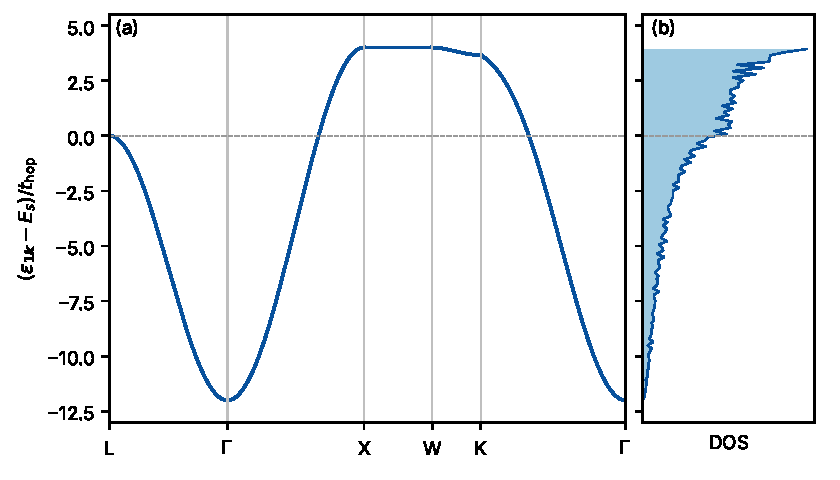
\includegraphics[width=0.75\linewidth]{figures/ch03/fig3_5.pdf}
  \caption{Tight-binding $s$ band of the face-centered cubic lattice, \cref{eq:3.2-fcc}: one orbital per site with on-site energy $E_s$, hopping $-t_{\mathrm{hop}}$ between the 12 nearest neighbors, no longer-range hopping, and the overlap between orbitals on different sites neglected. (a)~$(\varepsilon_{1\vect{k}} - E_s)/t_{\mathrm{hop}}$ along the path $\mathrm{L}$--$\mathrm{\Gamma}$--$\mathrm{X}$--$\mathrm{W}$--$\mathrm{K}$--$\mathrm{\Gamma}$, with $\mathrm{L} = (\tfrac12,\tfrac12,\tfrac12)$, $\mathrm{X} = (1,0,0)$, $\mathrm{W} = (1,\tfrac12,0)$ and $\mathrm{K} = (\tfrac34,\tfrac34,0)$ in units of $2\pi/a$. The band runs from $-12t_{\mathrm{hop}}$ at $\mathrm{\Gamma}$ to $+4t_{\mathrm{hop}}$, which it reaches at $\mathrm{X}$ and keeps along the line $\mathrm{X}$--$\mathrm{W}$; its value at $\mathrm{L}$ is $0$ and at $\mathrm{K}$ $3.66\,t_{\mathrm{hop}}$. (b)~Density of states, in arbitrary units, from a uniform grid of $160^3$ crystal momenta. Its peak at the top of the band comes from the flat line $\mathrm{X}$--$\mathrm{W}$.}
  \label{fig:3-tb}
\end{figure}

Silicon needs more than one orbital per atom, and the reason is chemical. A silicon atom has its $3s$ level several electronvolts below its $3p$ level, and in the crystal it uses both: it forms four bonds to the four neighbors of \cref{eq:3.1-basis}, at the corners of a tetrahedron. The orbitals that point along these bonds are the four $sp^3$ \emph{hybrids}
\begin{equation}
  \begin{aligned}
  h_1 &= \tfrac12(s + p_x + p_y + p_z), &\qquad h_2 &= \tfrac12(s + p_x - p_y - p_z), \\
  h_3 &= \tfrac12(s - p_x + p_y - p_z), &\qquad h_4 &= \tfrac12(s - p_x - p_y + p_z).
  \end{aligned}
  \label{eq:3.2-hybrids}
\end{equation}
These are orthonormal combinations of one $s$ and three $p$ orbitals on the same atom. Each is directed along one of the cube diagonals $(1,1,1)$, $(1,-1,-1)$, $(-1,1,-1)$ and $(-1,-1,1)$ that join an atom at $\vect{\tau}_1$ to its neighbors. Each hybrid has the on-site energy $(E_s + 3E_p)/4$, a quarter of the way from $E_p$ toward $E_s$. Forming the hybrids costs promotion energy, since an electron is moved from $s$ to $p$ character, and the bonds pay it back~\cite[Chap.~3]{harrison1980electronic}.

Two hybrids that point at each other across a bond, one on each atom, are coupled by a large matrix element, which we write $-V_{\mathrm{cov}}$ with $V_{\mathrm{cov}} > 0$ (Harrison's covalent energy). Treated alone, the pair is the two-orbital problem of \cref{sec:2.3}: a bonding combination $(h + h')/\sqrt2$ at $(E_s + 3E_p)/4 - V_{\mathrm{cov}}$ and an antibonding combination $(h - h')/\sqrt2$ at $(E_s + 3E_p)/4 + V_{\mathrm{cov}}$. A primitive cell holds two atoms and eight hybrids, which make four bonds, hence four bonding and four antibonding orbitals. Its eight valence electrons exactly fill the four bonding orbitals, two per bond, with opposite spins. The smaller couplings, between hybrids on the same atom and between neighboring bonds, then broaden the four bonding levels into four valence bands and the four antibonding levels into four conduction bands. The gap of silicon is the remnant of the bonding--antibonding splitting $2V_{\mathrm{cov}}$, reduced by these broadenings, and it survives because the splitting is larger than the bands are wide~\cite[Chap.~3]{harrison1980electronic}. This picture accounts for the count of \cref{sec:3.1}, four filled bands, without any reference to Bragg planes. It also explains where the valence charge sits: the bonding orbitals concentrate it between the atoms, in the bonds. This bond charge is not a sum of spherical atomic terms, and it gives the potential of silicon its (222) component; the (200) component stays zero by the glide symmetry (\cref{we:3-diamond}, \cref{app:C.17}). Germanium is bonded the same way, more weakly. In GaAs the two hybrids of a bond have different energies, the bond is partly ionic, and the gap is wider than the covalent splitting alone would give (\cref{sec:3.3}).

The nearly-free and the tight-binding pictures are two limits of the same problem, \cref{eq:3.2-Hk}, and both are approximations to it. Real valence states of silicon are well described by neither: they have the bonding character of the tight-binding picture, and the plane-wave content near the zone boundary that the nearly-free picture predicts. A first-principles calculation solves \cref{eq:3.2-Hk} in a plane-wave basis (\cref{sec:3.4,sec:3.5}), and Wannier functions (\cref{sec:3.6}) recover from it a set of localized orbitals in which the band structure has the tight-binding form of \cref{eq:3.2-LCAO}, with orthonormal orbitals and hopping integrals computed rather than guessed.

\subsection{The density vertex}

A dark-matter particle couples to the electrons through $n_e(\vect{q}) = \sum_j\ee^{\ii\vect{q}\cdot\vect{r}_j}$, and for independent electrons each transition moves one electron, with the single-particle matrix element $f_{i\to f}(\vect{q}) = \langle f|\ee^{\ii\vect{q}\cdot\vect{r}}|i\rangle$ of \cref{eq:2.2-ff} (\cref{eq:2.3-ph}). Between Bloch states this matrix element has a simple structure. Take $\psi_{n\vect{k}}$ as the initial state and $\psi_{m\vect{k}'}$ as the final one, with $\vect{k}$ and $\vect{k}'$ in the first zone. The momentum transfer lies on the same grid as the crystal momenta, since the dark-matter states are normalized in the same periodic box of volume $\Vol$ (\cref{sec:2.1}). With \cref{eq:3.2-bloch},
\begin{equation*}
  \langle\psi_{m\vect{k}'}|\ee^{\ii\vect{q}\cdot\vect{r}}|\psi_{n\vect{k}}\rangle
  = \frac1N\int_V\dd^3r\;\ee^{\ii(\vect{k}+\vect{q}-\vect{k}')\cdot\vect{r}}\,u^*_{m\vect{k}'}(\vect{r})\,u_{n\vect{k}}(\vect{r}) .
\end{equation*}
Split the crystal into cells, $\vect{r} = \vect{R} + \vect{x}$ with $\vect{x}$ in the cell at the origin. The product $u^*u$ is the same in every cell, and the phase factorizes into $\ee^{\ii(\vect{k}+\vect{q}-\vect{k}')\cdot\vect{R}}$ times its value at $\vect{x}$. The sum over cells is the lattice sum of \cref{eq:3.1-latticesum}, which equals $N$ if $\vect{k} + \vect{q} - \vect{k}'$ is a reciprocal-lattice vector $\vect{G}_{\mathrm{U}}$ and vanishes otherwise:
\begin{equation*}
  \langle\psi_{m\vect{k}'}|\ee^{\ii\vect{q}\cdot\vect{r}}|\psi_{n\vect{k}}\rangle
  = \delta_{\vect{k}',\,\vect{k}+\vect{q}-\vect{G}_{\mathrm{U}}}\int_\Omega\dd^3x\;\ee^{\ii\vect{G}_{\mathrm{U}}\cdot\vect{x}}\,u^*_{m\vect{k}'}(\vect{x})\,u_{n\vect{k}}(\vect{x}) .
\end{equation*}
This is the selection rule \cref{eq:3.1-selection}, now for one electron. The vector $\vect{G}_{\mathrm{U}}$ is the one that folds $\vect{k} + \vect{q}$ back into the first zone. It depends on $\vect{k}$ as well as on $\vect{q}$, and it is not in general the vector $\vect{G}_q$ nearest to $\vect{q}$ of \cref{eq:3.1-qsplit}. With the periodic gauge, $u_{m,\vect{k}+\vect{q}} = \ee^{-\ii\vect{G}_{\mathrm{U}}\cdot\vect{r}}u_{m\vect{k}'}$ by \cref{eq:A.5-periodic}, and the phase is absorbed into the final state:
\begin{keyresult}[Density vertex]
For $\vect{k}$ in the first zone and any $\vect{q}$, $\ee^{\ii\vect{q}\cdot\vect{r}}$ connects $\psi_{n\vect{k}}$ only to the states at crystal momentum $\vect{k} + \vect{q}$, folded back as $\vect{k}' = \vect{k} + \vect{q} - \vect{G}_{\mathrm{U}}$. The amplitude is the \emph{density vertex}
\begin{equation}
  \begin{aligned}
  \rho_{mn}(\vect{k},\vect{q}) &\equiv \langle\psi_{m,\vect{k}+\vect{q}}|\ee^{\ii\vect{q}\cdot\vect{r}}|\psi_{n\vect{k}}\rangle
  = \int_\Omega\dd^3r\;u^*_{m,\vect{k}+\vect{q}}(\vect{r})\,u_{n\vect{k}}(\vect{r}) \\
  &= \int_\Omega\dd^3r\;u^*_{m\vect{k}'}(\vect{r})\,\ee^{\ii\vect{G}_{\mathrm{U}}\cdot\vect{r}}\,u_{n\vect{k}}(\vect{r}),
  \end{aligned}
  \label{eq:3.2-rho}
\end{equation}
with $\rho_{nn}(\vect{k},0) = 1$. It is of order one and carries no factor of $N$. The Umklapp vector $\vect{G}_{\mathrm{U}}$ stays in the plane wave.
\end{keyresult}
The normalization $\rho_{nn}(\vect{k},0) = \int_\Omega|u_{n\vect{k}}|^2 = 1$ is that of \cref{eq:3.2-bloch}. The plane wave $\ee^{\ii\vect{G}_{\mathrm{U}}\cdot\vect{r}}$ in \cref{eq:3.2-rho} cannot be dropped. The overlap $\int_\Omega u^*_{m\vect{k}'}u_{n\vect{k}}$ without it is a different number, and it would make the vertex depend on $\vect{q}$ only through its reduced part. The crystal momentum changes by $\vect{q}$ modulo a reciprocal-lattice vector, but the wavefunction is probed by the whole $\vect{q}$, which is why \cref{sec:3.1} never folds it.

The plane-wave form of the vertex shows what happens to the momentum. We insert \cref{eq:3.2-pw} for both states in the cell integral of \cref{eq:3.2-rho} that carries $\ee^{\ii\vect{G}_{\mathrm{U}}\cdot\vect{r}}$. The cell integral of $\ee^{\ii(\vect{G}_{\mathrm{U}} + \vect{G} - \vect{G}')\cdot\vect{r}}$ is $\Omega\,\delta_{\vect{G}',\vect{G}+\vect{G}_{\mathrm{U}}}$, and
\begin{equation}
  \rho_{mn}(\vect{k},\vect{q}) = \sum_{\vect{G}}c^*_{m\vect{k}'}(\vect{G} + \vect{G}_{\mathrm{U}})\,c_{n\vect{k}}(\vect{G}),
  \qquad \vect{k}' = \vect{k} + \vect{q} - \vect{G}_{\mathrm{U}} .
  \label{eq:3.2-rhopw}
\end{equation}
Each plane-wave component of the initial state, with momentum $\vect{k} + \vect{G}$, is shifted by exactly $\vect{q}$ to $\vect{k}' + \vect{G} + \vect{G}_{\mathrm{U}}$, and the vertex is the overlap of the shifted state with the final one. Momentum is conserved component by component; the crystal only decides how the result is labeled. In the empty lattice, where each state is one plane wave, \cref{eq:3.2-rhopw} reduces to the momentum conservation of free electrons, and the distinction between normal and Umklapp processes is a matter of band labels. In a crystal the coefficients spread each state over many $\vect{G}$, and a large $|\vect{q}|$ picks out the overlap between the high-momentum tail of the initial state and the low-momentum part of the final one. In the notation of Ref.~\cite[Eqs.~(3.14)--(3.16)]{essig2016direct}, $c_{n\vect{k}}(\vect{G})$ is their $u_n(\vect{k} + \vect{G})$ and \cref{eq:3.2-rhopw} is their $f_{[n\vect{k},m\vect{k}',\vect{G}_{\mathrm{U}}]}$.

The vertices out of one state exhaust the probability. The periodic functions $u_{m,\vect{k}+\vect{q}}$, $m = 1, 2, \dots$, are the eigenfunctions of the Hermitian operator $H_{\vect{k}+\vect{q}}$ on one cell and form a complete orthonormal set there. Expanding $u_{n\vect{k}}$ in them and using its normalization,
\begin{equation}
  \sum_m|\rho_{mn}(\vect{k},\vect{q})|^2 = \sum_m\Bigl|\int_\Omega u^*_{m,\vect{k}+\vect{q}}\,u_{n\vect{k}}\Bigr|^2 = \int_\Omega|u_{n\vect{k}}|^2 = 1
  \label{eq:3.2-closure}
\end{equation}
for every $\vect{q}$. This is the closure relation of \cref{eq:2.2-closure} for a Bloch electron: a momentum transfer redistributes the electron over the bands at $\vect{k} + \vect{q}$ without changing its total weight. At small $q$ the weight stays in band $n$; at $q$ beyond a few reciprocal-lattice vectors it spreads over many high bands, and the transitions that a detector sees, into the conduction bands just above the gap, receive the fraction that \cref{we:3-vertex} illustrates.

In second quantization, \cref{eq:2.3-nq} in the Bloch basis becomes
\begin{equation}
  n_e(\vect{q}) = \sum_{s}\sum_{\vect{k}\in\mathrm{BZ}}\sum_{mn}\rho_{mn}(\vect{k},\vect{q})\,c^\dagger_{m,\vect{k}+\vect{q},s}\,c_{n\vect{k}s},
  \label{eq:3.2-ne}
\end{equation}
with $c_{m,\vect{k}+\vect{q},s} = c_{m\vect{k}'s}$ in the periodic gauge. The particle--hole matrix element of \cref{eq:2.3-ph} that takes an electron from a valence state $v\vect{k}$ to a conduction state $c\vect{k}'$ is $\rho_{cv}(\vect{k},\vect{q})$, and the independent-electron transition sum of \cref{eq:2.5-indep} becomes a sum of $|\rho_{cv}(\vect{k},\vect{q})|^2$ over $\vect{k}$, the valence and conduction bands, and spin. That sum, weighted by energy conservation, is the crystal form factor of Ref.~\cite[Eq.~(3.17)]{essig2016direct}, which \cref{sec:10.1} derives in the book's normalization. The counting of \cref{app:A.3} explains why no factor of $N$ appears in \cref{eq:3.2-rho}: one sum over $\vect{k}$ supplies a factor $N$, and the prefactor $2\pi/\Vol$ of the structure factor turns it into the intensive $2\pi/\Omega$.

\subsection{Velocity matrix elements}

Light of energy $\omega$ has the momentum $q = \omega$, a few electronvolts for visible and ultraviolet photons, and $10^{-3}$ of the zone size. Optical absorption probes the density vertex at small $q$, and there it is controlled by a second matrix element, that of the velocity. The momentum and velocity matrix elements between Bloch states at the same $\vect{k}$ are
\begin{equation}
  \begin{gathered}
  \vect{p}_{mn}(\vect{k}) = \langle\psi_{m\vect{k}}|\op{\vect{p}}|\psi_{n\vect{k}}\rangle = \int_\Omega\dd^3r\;u^*_{m\vect{k}}\,(\op{\vect{p}} + \vect{k})\,u_{n\vect{k}}, \\
  \vect{v}_{mn}(\vect{k}) = \langle\psi_{m\vect{k}}|\vect{v}|\psi_{n\vect{k}}\rangle, \qquad
  \vect{v} = \ii[H_{\mathrm{e}},\vect{r}] .
  \end{gathered}
  \label{eq:3.2-pv}
\end{equation}
The velocity operator is the time derivative of the position in the Heisenberg picture. For the local potential of \cref{eq:3.2-He}, $U(\vect{r})$ commutes with $\vect{r}$ and $\vect{v} = \op{\vect{p}}/m_e$, so that $\vect{v}_{mn} = \vect{p}_{mn}/m_e$. In plane waves, $\vect{p}_{mn}(\vect{k}) = \sum_{\vect{G}}c^*_{m\vect{k}}(\vect{G})(\vect{k} + \vect{G})c_{n\vect{k}}(\vect{G})$. The matrix elements of $\vect{r}$ itself between extended states are not defined as integrals over the crystal, but for $m \ne n$ the commutator gives them a meaning. Taking $\langle\psi_{m\vect{k}}|\cdot|\psi_{n\vect{k}}\rangle$ of $\vect{v} = \ii[H_{\mathrm{e}},\vect{r}]$,
\begin{equation}
  \langle\psi_{m\vect{k}}|\vect{r}|\psi_{n\vect{k}}\rangle = \frac{-\ii\,\vect{v}_{mn}(\vect{k})}{\varepsilon_{m\vect{k}} - \varepsilon_{n\vect{k}}}, \qquad m \ne n ,
  \label{eq:3.2-r}
\end{equation}
which is the form in which interband position matrix elements enter first-principles codes (\cref{app:E.4}).

The dependence of these matrix elements on $\vect{k}$ is easiest to handle through the operator $H_{\vect{k}}$ of \cref{eq:3.2-Hk}. Differentiating its definition, $\nabla_{\vect{k}}(\ee^{-\ii\vect{k}\cdot\vect{r}}H_{\mathrm{e}}\ee^{\ii\vect{k}\cdot\vect{r}}) = \ee^{-\ii\vect{k}\cdot\vect{r}}(-\ii\vect{r}H_{\mathrm{e}} + \ii H_{\mathrm{e}}\vect{r})\,\ee^{\ii\vect{k}\cdot\vect{r}}$, so
\begin{equation}
  \nabla_{\vect{k}}H_{\vect{k}} = \ee^{-\ii\vect{k}\cdot\vect{r}}\,\vect{v}\,\ee^{\ii\vect{k}\cdot\vect{r}}, \qquad
  \vect{v}_{mn}(\vect{k}) = \int_\Omega\dd^3r\;u^*_{m\vect{k}}\,(\nabla_{\vect{k}}H_{\vect{k}})\,u_{n\vect{k}} .
  \label{eq:3.2-dHk}
\end{equation}
For the local potential, $\nabla_{\vect{k}}H_{\vect{k}} = (\op{\vect{p}} + \vect{k})/m_e$; the identity holds for any Hamiltonian, nonlocal ones included. The group velocity and the $\vect{k}\cdot\vect{p}$ relation both follow by differentiating $H_{\vect{k}}u_{n\vect{k}} = \varepsilon_{n\vect{k}}u_{n\vect{k}}$ with respect to $\vect{k}$,
\begin{equation*}
  (\nabla_{\vect{k}}H_{\vect{k}})\,u_{n\vect{k}} + H_{\vect{k}}\nabla_{\vect{k}}u_{n\vect{k}} = (\nabla_{\vect{k}}\varepsilon_{n\vect{k}})\,u_{n\vect{k}} + \varepsilon_{n\vect{k}}\nabla_{\vect{k}}u_{n\vect{k}},
\end{equation*}
and projecting onto $u_{m\vect{k}}$. For $m = n$ the terms with $\nabla_{\vect{k}}u_{n\vect{k}}$ cancel, because $\langle u_{n\vect{k}}|H_{\vect{k}} = \varepsilon_{n\vect{k}}\langle u_{n\vect{k}}|$, and normalization leaves
\begin{keyresult}[Group velocity]
\begin{equation}
  \vect{v}^{\mathrm{g}}_n(\vect{k}) \equiv \nabla_{\vect{k}}\varepsilon_{n\vect{k}} = \vect{v}_{nn}(\vect{k}) .
  \label{eq:3.2-vg}
\end{equation}
The slope of a band is the expectation value of the velocity in the Bloch state.
\end{keyresult}
This is the Hellmann--Feynman theorem for the parameter $\vect{k}$. A wave packet built from states of band $n$ near $\vect{k}$ moves with $\vect{v}^{\mathrm{g}}_n$, the \emph{group velocity}~\cite[Chap.~8 and App.~E]{ashcroft1976solid}. For free electrons it is $\vect{k}/m_e$. On a Bragg plane its component along $\vect{G}$ vanishes, as the standing waves of the nearly-free picture require, and in the tight-binding band \cref{eq:3.2-fcc} it vanishes at $\mathrm{\Gamma}$, $\mathrm{X}$ and $\mathrm{L}$ and is at most of order $t_{\mathrm{hop}}a$. For $m \ne n$, and $\varepsilon_{m\vect{k}} \ne \varepsilon_{n\vect{k}}$, the projection gives instead
\begin{equation}
  \langle u_{m\vect{k}}|\nabla_{\vect{k}}u_{n\vect{k}}\rangle = \frac{\vect{v}_{mn}(\vect{k})}{\varepsilon_{n\vect{k}} - \varepsilon_{m\vect{k}}} ,
  \label{eq:3.2-dudk}
\end{equation}
the first-order change of $u_{n\vect{k}}$ along band $m$ when $\vect{k}$ moves; this is $\vect{k}\cdot\vect{p}$ perturbation theory~\cite[Chap.~2]{yu2010fundamentals}.

The optical limit of the vertex is now one line. Expand the final state, $u_{m,\vect{k}+\vect{q}} = u_{m\vect{k}} + \vect{q}\cdot\nabla_{\vect{k}}u_{m\vect{k}} + O(q^2)$, in the overlap $\int_\Omega u^*_{m,\vect{k}+\vect{q}}u_{n\vect{k}}$ of \cref{eq:3.2-rho}. The zeroth-order term $\langle u_{m\vect{k}}|u_{n\vect{k}}\rangle$ vanishes for $m \ne n$, and the first-order term is $\vect{q}\cdot\langle\nabla_{\vect{k}}u_{m\vect{k}}|u_{n\vect{k}}\rangle = \vect{q}\cdot\langle u_{n\vect{k}}|\nabla_{\vect{k}}u_{m\vect{k}}\rangle^*$. With \cref{eq:3.2-dudk}, with $n$ and $m$ exchanged, and the hermiticity of the velocity, $\vect{v}^*_{nm} = \vect{v}_{mn}$:
\begin{keyresult}[Optical limit of the density vertex]
\begin{equation}
  \rho_{mn}(\vect{k},\vect{q}) = \frac{\vect{q}\cdot\vect{v}_{mn}(\vect{k})}{\varepsilon_{m\vect{k}} - \varepsilon_{n\vect{k}}} + O(q^2), \qquad m \ne n .
  \label{eq:3.2-optical}
\end{equation}
An interband vertex vanishes linearly as $q \to 0$, with a slope set by the velocity matrix element and the transition energy. The intraband vertex tends to one, $\rho_{nn}(\vect{k},\vect{q}) = 1 + O(q)$.
\end{keyresult}
The same result follows from expanding the plane wave, $\ee^{\ii\vect{q}\cdot\vect{r}} \simeq 1 + \ii\vect{q}\cdot\vect{r}$, between states at the same $\vect{k}$, and using \cref{eq:3.2-r}, which is the route of \cref{eq:A.5-optical}. The expansion assumes that the phases of the states are chosen smoothly in $\vect{k}$ between $\vect{k}$ and $\vect{k} + \vect{q}$. Any other choice multiplies both sides of \cref{eq:3.2-optical} by phases (\cref{eq:A.5-gauge}), and leaves $|\rho_{mn}|^2$, which is what a first-order rate contains, unchanged. When band $m$ is degenerate at $\vect{k}$, only the sum of $|\rho_{mn}|^2$ over the degenerate partners is defined (\cref{app:A.5}).

The interband probability $|\rho_{mn}|^2$ therefore grows as $q^2$ at small $q$, like the dipole transition $1s \to 2p$ of hydrogen in \cref{sec:2.2}. The intraband vertex does not vanish, but in a full band it cannot act: the state at $\vect{k} + \vect{q}$ in the same band is occupied, and the term is Pauli blocked. Intraband transitions matter in metals, at the Fermi surface (\cref{sec:4.5}). For photons, \cref{eq:3.2-optical} is all that is needed. The absorption spectrum of a semiconductor is a sum over the squared components of $\vect{v}_{cv}(\vect{k})$ along the polarization of the light (\cref{sec:4.4,sec:4.6}). Absorbed bosonic dark matter, whose momentum is also far below the zone scale (\cref{sec:3.3}), is governed by the same matrix elements (\cref{sec:10.7}).

The expansion of $u_{m,\vect{k}+\vect{q}}$ is useful while its first-order term is small, and by \cref{eq:3.2-dudk} this requires
\begin{equation}
  q \ll \frac{|\varepsilon_{m\vect{k}} - \varepsilon_{n\vect{k}}|}{|\vect{v}_{mn}(\vect{k})|} .
  \label{eq:3.2-validity}
\end{equation}
For a photon, with $q = \omega \simeq |\varepsilon_{m\vect{k}} - \varepsilon_{n\vect{k}}|$, the condition reads $|\vect{v}_{mn}| \ll 1$, the speed of light, and it always holds. For dark matter that deposits the same energy, the momentum transfer is at least $\omega/v_{\mathrm{max}}$ (\cref{sec:1.3}), and the condition becomes $|\vect{v}_{mn}| \ll v_{\mathrm{max}} = 2.650\times10^{-3}$. Valence electrons, however, move with typical velocities $\sim\alpha$, and the Fermi velocity of silicon's valence density is $7.0\times10^{-3}$ (\cref{sec:2.5}). Parametrically, then, the momentum transfers at which dark matter can excite an electron across the gap lie at or beyond the edge of the optical limit. \Cref{eq:3.2-optical} is a check on a calculation of $\rho_{mn}$ at small $q$, and a scattering rate needs the full vertex of \cref{eq:3.2-rhopw}.

In practice, the band energies $\varepsilon_{n\vect{k}}$ and the periodic parts $u_{n\vect{k}}$ of a real material come from density-functional theory (\cref{sec:3.4}). A code solves \cref{eq:3.2-central} for the Kohn--Sham potential in a basis of plane waves up to a cutoff (\cref{sec:3.5}) and stores the coefficients $c_{n\vect{k}}(\vect{G})$ on a grid of crystal momenta. The vertex is then the sum \cref{eq:3.2-rhopw}, with the coefficients of the two states matched by the integer coordinates of their $\vect{G}$. For all $\vect{G}_{\mathrm{U}}$ at once it is a fast Fourier transform of the product $u^*_{m\vect{k}'}u_{n\vect{k}}$, and the momentum matrix element is the corresponding sum over $\vect{k} + \vect{G}$ (\cref{app:E.7}). The pseudopotentials of these codes are nonlocal, and then $\vect{v} \neq \op{\vect{p}}/m_e$: by \cref{eq:3.2-dHk}, $\vect{v}_{mn}$ acquires the derivative of the nonlocal potential with respect to $\vect{k}$, a correction that \cref{app:E.7} evaluates and that changes the computed absorption of diamond by \SIrange{15}{20}{\percent}~\cite[Fig.~1]{ismailbeigi2001coupling}.

\begin{workedexample}{The vertex between the two lowest nearly-free bands}\label{we:3-vertex}
Return to the one-dimensional crystal of \cref{we:3-gap1d}, and take the initial state at the left zone boundary, $k = -\pi/a = -G_1/2$, in the lowest band, with the final state in the second band. Near the boundary the two bands are made of the plane waves $\ee^{\ii kx}$ and $\ee^{\ii(k+G_1)x}$, and \cref{eq:3.2-twowave}, with $\vect{G} \to -G_1$, mixes them. Its lower eigenvector is $(c(0), c(G_1)) = (\cos\theta_k, \sin\theta_k)$ and its upper one $(-\sin\theta_k, \cos\theta_k)$, with $\tan2\theta_k = 2|U_{G_1}|/(\varepsilon^0_{k+G_1} - \varepsilon^0_k)$; for $U_{G_1} < 0$ both components of the lower state have the same sign. At the boundary the two free energies are equal and $\theta = \pi/4$.

\emph{Small $q$.} For $0 < q < G_1$, $k + q$ stays in the first zone, $\vect{G}_{\mathrm{U}} = 0$, and \cref{eq:3.2-rhopw} reads $\rho_{21}(k,q) = -\sin\theta_{k+q}\cos\theta_k + \cos\theta_{k+q}\sin\theta_k = \sin(\theta_k - \theta_{k+q})$. With $\varepsilon^0_{k+G_1} - \varepsilon^0_k = G_1(k + G_1/2)/m_e$, the angle falls from $\pi/4$ with the slope $\dd\theta/\dd k = -G_1/(4m_e|U_{G_1}|)$ at the boundary, and
\begin{equation*}
  |\rho_{21}(k,q)| \simeq \frac{qG_1}{4m_e|U_{G_1}|} = \frac{q}{\SI{448}{eV}} .
\end{equation*}
The optical limit agrees. In the two-wave model $|v_{21}| = G_1/2m_e = 2.23\times10^{-3}$, the velocity of a free electron at the zone boundary, and \cref{eq:3.2-optical} gives $q|v_{21}|/2|U_{G_1}|$, the same expression. The full calculation of \cref{fig:3-nfe}(b) has $|v_{21}| = 2.24\times10^{-3}$ and $\varepsilon_{2k} - \varepsilon_{1k} = \SI{0.998}{eV}$. At $q = \SI{10}{eV}$ the vertex is $0.0225$ in the full calculation and in the optical limit; at \SI{100}{eV} the two are 0.210 and 0.225. At $q = 2|U_{G_1}|/v_{\mathrm{max}} = \SI{377}{eV}$, the smallest momentum transfer with which dark matter can deposit the \SI{1}{eV} gap, the full vertex is 0.496 and the optical limit 0.849, too large by a factor of 1.7, and $|\rho_{21}|^2$ by a factor of 2.9. This $q$ is a reference scale, not an allowed event, since the vertex is evaluated at fixed $k$: at $q = \SI{377}{eV}$ the final state from this $k$ has moved up the second band, the transition costs \SI{1.6}{eV}, and depositing \SI{1.6}{eV} needs $q \ge \SI{0.61}{keV}$. The vertex saturates instead of growing: as $k + q$ moves away from the boundary, the final state becomes a single plane wave, and $|\rho_{21}|$ tends to $\sin(\pi/4) = 0.71$ in the two-wave model. The scale on which the linear law fails, $4m_e|U_{G_1}|/G_1 = \SI{448}{eV}$, is the $|\varepsilon_{2k} - \varepsilon_{1k}|/|v_{21}|$ of \cref{eq:3.2-validity}, and $|v_{21}| = 0.85\,v_{\mathrm{max}}$ puts the momentum transfers of dark matter right at it.

\emph{Umklapp.} Now take $q = G_1 = \SI{2.28}{keV}$. Then $k + q = +\pi/a$, which is folded back to $k' = -\pi/a$ with $\vect{G}_{\mathrm{U}} = G_1$: the final state has the same reduced crystal momentum as the initial one, and the transition energy is the same \SI{0.998}{eV} as at $q \to 0$. At the boundary the states are $(c(0), c(G_1)) = (1, 1)/\sqrt2$ in band 1 and $(-1, 1)/\sqrt2$ in band 2. In \cref{eq:3.2-rhopw} only the term $\vect{G} = 0$ survives in the two-wave model, $c^*_{2k'}(G_1)\,c_{1k}(0) = \tfrac12$, so $|\rho_{21}(k, G_1)| = \tfrac12$; the full calculation finds 0.501. The same pair of states, with the same transition energy, has the vertex 0.02 at $q = \SI{10}{eV}$ and 0.50 at $q = G_1$. The difference comes from $\vect{G}_{\mathrm{U}}$ in the plane wave: the momentum transfer $G_1$ moves the component $\ee^{\ii kx}$ of the initial state onto the component $\ee^{\ii(k'+G_1)x}$ of the final one, and these overlap at order one. In the two-wave model band 2 receives a quarter of the probability and band 1 keeps another quarter. The remaining half, from the component $\ee^{\ii(k+G_1)x}$ shifted to $\ee^{\ii(k+2G_1)x}$, goes into bands 3 and 4, whose energies at the boundary are near $(3G_1/2)^2/2m_e = \SI{11.5}{eV}$. The full calculation finds $|\rho_{m1}|^2 = 0.298$, 0.251, 0.226 and 0.225 for $m = 1$ to 4, and the closure relation \cref{eq:3.2-closure} holds to $10^{-10}$.
\end{workedexample}

A one-dimensional cosine potential has two parameters and silicon has many. The lessons carry over, however: interband vertices are suppressed as $q$ at small momentum transfer, they saturate on the scale where the states change across the zone, and an Umklapp vector in the plane wave can make them of order one. Where the band edges of silicon, germanium and GaAs lie, and how large the relevant velocities and gaps are, is the subject of \cref{sec:3.3}.

\section{Silicon, germanium and gallium arsenide}\label{sec:3.3}

The highest occupied electron state of silicon sits at the center of the Brillouin zone, and the lowest empty one sits \SI{85}{\percent} of the way to the square face of the zone, at a crystal momentum of \SI{1.94}{keV}. A photon with the \SI{1.17}{eV} needed to cross the gap carries a momentum a thousand times smaller and cannot connect the two states by itself. A dark-matter particle that scatters with a momentum transfer of a few keV can. Which momentum transfers reach which excitation energies is the target's half of the kinematic question of \cref{sec:1.3}, and the answer lies in the bands just below and just above the gap. \Cref{tab:3-materials} collects the band edges, effective masses and spin--orbit splittings of silicon, germanium and GaAs, the book's running materials.

\subsection{Band edges and valleys}

At the temperatures at which detectors run, the four lowest bands of silicon are full and all higher bands are empty (\cref{sec:3.2}). The full bands are the \emph{valence bands} and the empty ones the \emph{conduction bands}. We label them with the subscripts $v$ and $c$, as in $\varepsilon_{v\vect{k}}$ and $\varepsilon_{c\vect{k}}$, and the two letters never appear on their own. The highest valence energy is the \emph{valence-band maximum} (VBM), and the lowest conduction energy the \emph{conduction-band minimum} (CBM). The band gap is the distance between the two,
\begin{equation}
  \Eg = \min_{c,\vect{k}}\varepsilon_{c\vect{k}} - \max_{v,\vect{k}}\varepsilon_{v\vect{k}} ,
  \label{eq:3.3-Eg}
\end{equation}
wherever in the zone the two extremes occur. When they occur at different crystal momenta the gap is \emph{indirect}. A transition at fixed crystal momentum is called \emph{vertical}, after its appearance in a band diagram, and the smallest vertical transition energy is the \emph{minimum direct gap},
\begin{equation}
  E_{\mathrm{dir}} = \min_{v,c,\vect{k}}\left(\varepsilon_{c\vect{k}} - \varepsilon_{v\vect{k}}\right) \ge \Eg .
  \label{eq:3.3-Edir}
\end{equation}
In a direct-gap crystal the two are equal.

\Cref{fig:3-si-bands}(a) shows the bands of silicon along the lines of \cref{sec:3.1}. The VBM lies at $\mathrm{\Gamma}$ and is threefold degenerate, sixfold with spin. These are the bonding states of the $sp^3$ picture of \cref{sec:3.2} with pure $p$ character: the three states transform like $x$, $y$ and $z$ under the rotations of the crystal, and an $s$ orbital, unchanged by every rotation, cannot enter them. The CBM lies on the line from $\mathrm{\Gamma}$ to $\mathrm{X}$, at the crystal momentum
\begin{equation}
  \vect{k}_{\mathrm{c}} = 0.85\,\frac{2\pi}{a}\,(1, 0, 0)
  \label{eq:3.3-kc}
\end{equation}
and at the five equivalent points along $\pm x$, $\pm y$ and $\pm z$; the position was measured by electron--nuclear double resonance on donor electrons, which occupy these states~\cite{feher1959electron}. The six minima are the \emph{valleys} of the conduction band. An electron excited across the gap relaxes into one of them, and near its bottom it behaves like a free particle with an anisotropic mass, which we derive below. The gap is $\Eg = \SI{1.17}{eV}$ at low temperature, $\SI{1.1692}{eV}$ in the extrapolation to zero temperature~\cite[Eq.~(11)]{ramanathan2020ionization}, and \SI{1.12}{eV} at \SI{300}{K}~\cite[Table~I]{lucero2012improved}. It shrinks on warming because the lattice expands and the electron--phonon interaction renormalizes the band energies (\cref{sec:13.7}). The vertical transitions of silicon cost much more. The smallest, $E_{\mathrm{dir}} = \SI{3.4}{eV}$, joins the valence and conduction states at $\mathrm{\Gamma}$~\cite[Table~II]{rideau2006strained}, and vertical transitions near $\mathrm{L}$ start only slightly higher, at \SI{3.45}{eV}~\cite[Table~VI]{rideau2006strained}. Silicon is thus indirect by a wide margin, $E_{\mathrm{dir}} \approx 3\Eg$.

\begin{figure}[tbp]
  \centering
  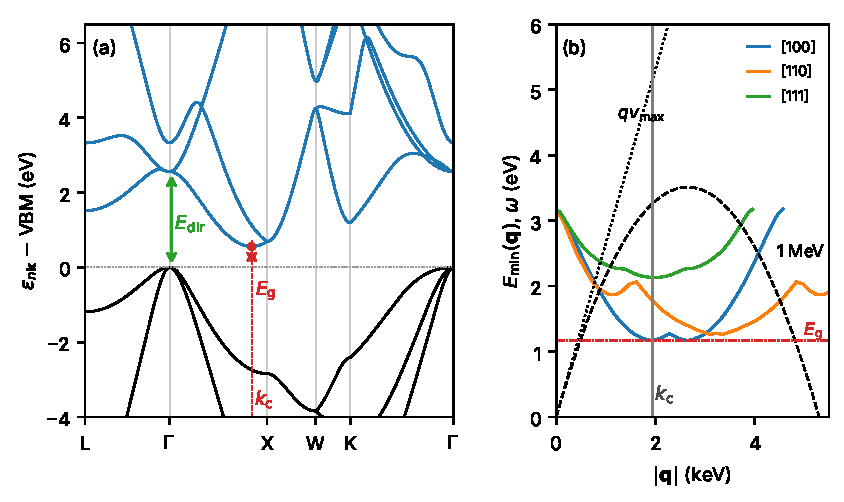
\includegraphics[width=\linewidth]{figures/ch03/fig3_6.pdf}
  \caption{Silicon. (a)~Band structure along $\mathrm{L}$--$\mathrm{\Gamma}$--$\mathrm{X}$--$\mathrm{W}$--$\mathrm{K}$--$\mathrm{\Gamma}$ (points of \cref{sec:3.1}), valence bands black and conduction bands blue, energies from the valence-band maximum. The bands are the Kohn--Sham bands of the plane-wave calculation of \cref{app:E.1} at the measured lattice constant: generalized-gradient functional of Perdew, Burke and Ernzerhof (PBE), SG15 norm-conserving pseudopotential, cutoff \SI{60}{Ry}, $12^3$ grid for the density, $a = \SI{5.431}{\angstrom}$, no spin--orbit coupling~\cite{giannozzi2017advanced,hamann2013optimized,schlipf2015optimization}. They put the conduction-band minimum at $k_{\mathrm{c}} = 0.843\,(2\pi/a)$ (measured $0.85$) and the indirect gap $\Eg$ at \SI{0.557}{eV} (measured \SI{1.17}{eV}), the gap problem of density-functional theory. The vertical gap at $\mathrm{\Gamma}$, marked $E_{\mathrm{dir}}$, is \SI{2.56}{eV} (measured \SI{3.4}{eV}) and is the smallest vertical gap in the zone; the one at $\mathrm{L}$ is \SI{2.70}{eV} (measured \SI{3.45}{eV}). (b)~Minimum pair energy $E_{\mathrm{min}}(\vect{q})$, \cref{eq:3.3-Emin}, for $\vect{q}$ along [100], [110] and [111], from the same calculation on a grid of $48^3$ crystal momenta, with the conduction bands shifted rigidly up by \SI{0.61}{eV} (a scissor, \cref{sec:3.4}) so that the indirect gap equals the measured \SI{1.17}{eV} (dash-dotted line); at $\vect{q} = 0$ the shifted bands give $E_{\mathrm{min}} = \SI{3.17}{eV}$. Dashed: the largest energy that dark matter of \SI{1}{MeV} can deposit, $qv_{\mathrm{max}} - q^2/2\mchi$; dotted: the bound $qv_{\mathrm{max}}$ for any mass, with $v_{\mathrm{max}} = 2.650\times10^{-3}$. The vertical line marks $|\vect{k}_{\mathrm{c}}| = \SI{1.94}{keV}$. Along [100], $E_{\mathrm{min}}$ returns to its value at $\vect{q} = 0$ at $|\vect{G}_{200}| = \SI{4.57}{keV}$.}
  \label{fig:3-si-bands}
\end{figure}

Germanium has the same diamond structure, with $a = \SI{5.658}{\angstrom}$ at room temperature~\cite[Sect.~II\,A]{rideau2006strained}, and the same threefold VBM at $\mathrm{\Gamma}$. Its CBM, however, lies at $\mathrm{L}$, the center of a hexagonal face of the zone (\cref{fig:3-ge-gaas}(a)). The eight $\mathrm{L}$ points come in pairs that differ by a vector $\vect{G}_{111}$ and are the same crystal momentum, so germanium has four valleys, each made of two half-ellipsoids on opposite faces of the zone. The gap is \SI{0.744}{eV} at low temperature~\cite[Table~VI]{rideau2006strained} and \SI{0.66}{eV} at \SI{300}{K}~\cite[Table~I]{lucero2012improved}. The conduction state at $\mathrm{\Gamma}$ is only \SI{0.15}{eV} higher, $E_{\mathrm{dir}} = \SI{0.89}{eV}$~\cite[Table~II]{rideau2006strained}: germanium is indirect by a narrow margin, and a calculation can easily get the order of the two states wrong.

GaAs has the zincblende structure, with $a = \SI{5.653}{\angstrom}$ at room temperature~\cite{vurgaftman2001band}, and both band edges at $\mathrm{\Gamma}$ (\cref{fig:3-ge-gaas}(b)). Its gap is direct, \SI{1.52}{eV} at low temperature and \SI{1.42}{eV} at \SI{300}{K}~\cite[Table~I]{lucero2012improved}, and the conduction band has a single, isotropic valley. Valleys at $\mathrm{L}$ and $\mathrm{X}$ follow at 1.815 and \SI{1.981}{eV}, 0.30 and \SI{0.46}{eV} above the minimum~\cite{vurgaftman2001band}. Gallium and arsenic flank germanium in the periodic table, yet the gap of GaAs is twice that of germanium. The difference comes from the partly ionic bond of \cref{sec:3.2}: the two hybrids of a bond have different energies, and this difference adds to their covalent splitting.

\begin{figure}[tbp]
  \centering
  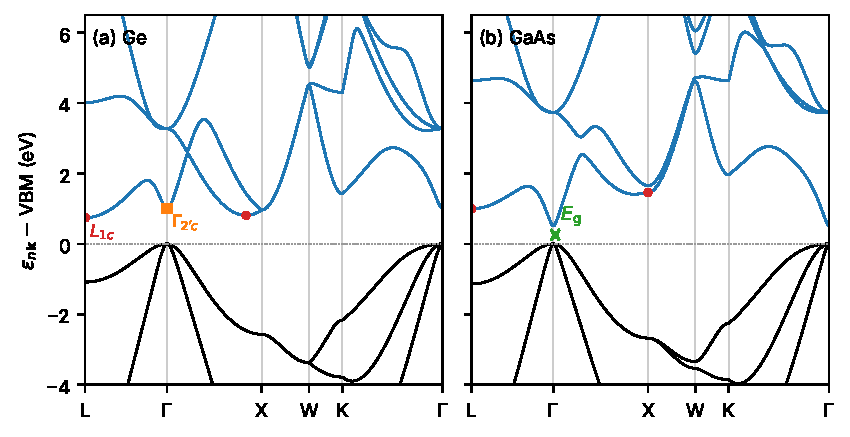
\includegraphics[width=\linewidth]{figures/ch03/fig3_7.pdf}
  \caption{Band structures of (a)~germanium and (b)~GaAs along the path of \cref{fig:3-si-bands}(a). Energies from the valence-band maximum; red dots mark the lowest conduction states away from $\mathrm{\Gamma}$. (a)~Local empirical pseudopotential of Cohen and Bergstresser~\cite{cohen1966band} at $a = \SI{5.66}{\angstrom}$, the lattice constant of their fit, without spin--orbit coupling, with the conduction bands shifted down by \SI{0.21}{eV} so that the $\mathrm{L}$ minimum sits at the measured \SI{0.744}{eV}. The crystal is indirect, with the $s$-like state $\mathrm{\Gamma}_{2'c}$ (square) at \SI{1.01}{eV} (measured \SI{0.89}{eV}) and the $\Delta$ minimum, at $0.83\,(2\pi/a)$ along $\mathrm{\Gamma}$--$\mathrm{X}$, at \SI{0.81}{eV}. Plain PBE with spin--orbit coupling at the measured lattice constant closes the germanium gap, with $\mathrm{\Gamma}_{7c}$ \SI{0.05}{eV} below the valence maximum. (b)~PBE plane-wave calculation of \cref{fig:3-si-bands} (SG15 pseudopotentials with the Ga $3d$ shell in the valence, \SI{60}{Ry}, $12^3$ grid, no spin--orbit coupling) at the room-temperature lattice constant $a = \SI{5.653}{\angstrom}$~\cite{giannozzi2017advanced,hamann2013optimized,schlipf2015optimization}. The gap is direct, as measured, but PBE underestimates it: \SI{0.51}{eV} against the measured \SI{1.52}{eV} at low temperature, with the $\mathrm{L}$ and $\mathrm{X}$ states at 1.00 and \SI{1.46}{eV} (measured 1.815 and \SI{1.981}{eV}).}
  \label{fig:3-ge-gaas}
\end{figure}

The bands in \cref{fig:3-si-bands} and \cref{fig:3-ge-gaas}(b) come from density-functional theory, which yields the potential from the electron density. A second route, which we use for the germanium bands of \cref{fig:3-ge-gaas}(a) and below as a model to test the velocity sum rules, is the empirical pseudopotential. It solves the central equation \cref{eq:3.2-central} with a potential that has nonzero Fourier components $U_{\vect{G}}$ on just the three shortest shells of reciprocal-lattice vectors, and fits these three numbers per element to measured optical transitions~\cite{cohen1966band}. That the fit works at all shows how much of the band structure the lattice fixes and how little of the potential it needs; the price is that the potential is not computed but adjusted, and it says nothing about wavefunctions at large momentum. Its potential is local, which is what makes it a convenient test bed for the sum rules. The band parameters of \cref{tab:3-materials} are measured. A first-principles calculation is checked against exactly these numbers: the measured gaps, the valley positions, the masses from cyclotron resonance, and the electronic dielectric constant of silicon, $\varepsilon_\infty = 11.7$, the square of its long-wavelength refractive index, 3.42~\cite{li1980refractive} (\cref{sec:4.4}). For the gaps the comparison needs one more step, a \emph{quasiparticle correction} that turns the Kohn--Sham eigenvalues into the energies to add or remove an electron (\cref{app:E.3}). The PBE functional of \cref{fig:3-si-bands} is \emph{semilocal}: its exchange--correlation energy at each point depends on the density and its gradient there and nowhere else. It places the CBM of silicon at $k_{\mathrm{c}} = 0.843\,(2\pi/a)$ and its longitudinal mass, $0.95\,m_e$, within \SI{4}{\percent} of experiment, but it puts the gap at \SI{0.56}{eV}, half the measured one.

\begin{table}[tbp]
  \centering
  \caption{Band parameters of silicon, germanium and GaAs. Lattice constant $a$ at room temperature: silicon~\cite[lattice parameter of silicon]{mohr2025codata}, germanium~\cite[Sect.~II\,A]{rideau2006strained}, GaAs~\cite{vurgaftman2001band}. Gaps at low temperature: silicon~\cite[Eq.~(11)]{ramanathan2020ionization}, germanium~\cite[Table~VI]{rideau2006strained}, GaAs~\cite[Table~I]{lucero2012improved}; at \SI{300}{K}~\cite[Table~I]{lucero2012improved}. Minimum direct gaps $E_{\mathrm{dir}}$ and spin--orbit splittings $\Delta_{\mathrm{SO}}$ of silicon and germanium~\cite[Table~II]{rideau2006strained}. Conduction valleys: position and number; masses along ($m^*_\parallel$) and across ($m^*_\perp$) the valley axis, silicon~\cite{hensel1965cyclotron} as listed in Ref.~\cite[Table~VII]{rideau2006strained}, germanium~\cite[Table~VII]{rideau2006strained}. Heavy- and light-hole masses $m_{\mathrm{hh}}$, $m_{\mathrm{lh}}$ along [100] and [111] from \cref{eq:3.3-holes} with the Luttinger parameters $(\gamma^{\mathrm{Lu}}_1, \gamma^{\mathrm{Lu}}_2, \gamma^{\mathrm{Lu}}_3) = (4.285, 0.339, 1.446)$ for silicon and $(13.25, 4.20, 5.56)$ for germanium~\cite[Table~VII]{rideau2006strained}, and $(6.98, 2.06, 2.93)$ for GaAs. All GaAs entries not credited otherwise are from Ref.~\cite{vurgaftman2001band}. Masses in units of $m_e$.}
  \label{tab:3-materials}
  \small
  \begin{tabular}{l ccc}
    \toprule
    & Si & Ge & GaAs \\
    \midrule
    $a$ (\AA) & 5.431 & 5.658 & 5.653 \\
    $\Eg$, low $T$ / \SI{300}{K} (eV) & 1.17 / 1.12 & 0.744 / 0.66 & 1.52 / 1.42 \\
    gap & indirect & indirect & direct \\
    $E_{\mathrm{dir}}$ (eV) & 3.4 & 0.89 & 1.52 \\
    valleys & $0.85\,\mathrm{X}$, 6 & $\mathrm{L}$, 4 & $\mathrm{\Gamma}$, 1 \\
    $m^*_\parallel$ / $m^*_\perp$ & 0.916 / 0.191 & 1.59 / 0.0815 & 0.067 (isotropic) \\
    $\Delta_{\mathrm{SO}}$ (eV) & 0.044 & 0.296 & 0.341 \\
    $m_{\mathrm{hh}}$ [100] / [111] & 0.277 / 0.718 & 0.206 / 0.469 & 0.350 / 0.893 \\
    $m_{\mathrm{lh}}$ [100] / [111] & 0.201 / 0.139 & 0.046 / 0.041 & 0.090 / 0.078 \\
    \bottomrule
  \end{tabular}
\end{table}

A gap of an electronvolt is enormous compared with the temperature of a detector, and the number of electrons excited across it by heat alone is a useful check of what ``empty'' means. Far from the chemical potential $\mu_{\mathrm{ch}}$ the occupation \cref{eq:3.2-fnk} of a conduction state is the Boltzmann factor $\ee^{-(\varepsilon_{c\vect{k}} - \mu_{\mathrm{ch}})/T}$. For a parabolic band of mass $m$ its sum over crystal momenta, $\int\dd^3k\,(2\pi)^{-3}\ee^{-k^2/2mT} = (mT/2\pi)^{3/2}$, times 2 for spin, gives the electron density $2(m_{\mathrm{dc}}T/2\pi)^{3/2}$ times the Boltzmann factor of the CBM. The empty valence states, the holes, give the same expression with the valence mass and the factor $\ee^{-(\mu_{\mathrm{ch}} - \varepsilon_{\mathrm{VBM}})/T}$. In a pure crystal the two densities are equal, the chemical potential drops out of their product, and the \emph{intrinsic carrier density} is~\cite[Chap.~28]{ashcroft1976solid}
\begin{equation}
  \nd_{\mathrm{i}} = 2\left(\frac{T}{2\pi}\right)^{3/2}(m_{\mathrm{dc}}m_{\mathrm{dv}})^{3/4}\,\ee^{-\Eg/2T} .
  \label{eq:3.3-ni}
\end{equation}
Here $m_{\mathrm{dc}}$ and $m_{\mathrm{dv}}$ are the density-of-states masses of the conduction and valence bands: for silicon $m_{\mathrm{dc}} = 6^{2/3}(m^*_\parallel m^{*2}_\perp)^{1/3} = 1.06\,m_e$, which counts the six valleys, and $m_{\mathrm{dv}} = (m_{\mathrm{hh}}^{3/2} + m_{\mathrm{lh}}^{3/2})^{2/3} = 0.50\,m_e$, which adds the heavy and light holes with their spherically averaged masses $m_e/(\gamma^{\mathrm{Lu}}_1 \mp 2\bar\gamma^{\mathrm{Lu}})$, $\bar\gamma^{\mathrm{Lu}} = (2\gamma^{\mathrm{Lu}}_2 + 3\gamma^{\mathrm{Lu}}_3)/5$, from the Luttinger parameters of \cref{eq:3.3-holes} below. At \SI{300}{K}, with $\Eg = \SI{1.12}{eV}$, \cref{eq:3.3-ni} yields $\nd_{\mathrm{i}} \approx \SI{6e9}{cm^{-3}}$ for parabolic bands. With the low-temperature gap it falls to $10^{-20}\,\si{cm^{-3}}$ at \SI{77}{K} and to $10^{-720}\,\si{cm^{-3}}$ at \SI{4}{K}. A kilogram of silicon has a volume of \SI{429}{cm^3}, so a cold crystal holds no thermally excited carriers at all, and the dark counts of a charge detector (\cref{sec:1.5}) come from other sources.

\subsection{Effective masses from \texorpdfstring{$\vect{k}\cdot\vect{p}$}{k.p} theory}

Near the bottom of a valley the band is a quadratic function of the distance $\delta\vect{k} = \vect{k} - \vect{k}_0$ from the minimum $\vect{k}_0$. Its curvature decides how an electron there moves, and how many states lie within an energy $\omega$ of the edge. The curvature follows from the states at $\vect{k}_0$ alone. With \cref{eq:3.2-Hk}, the Bloch Hamiltonian a little away from $\vect{k}_0$ is
\begin{equation*}
  H_{\vect{k}_0+\delta\vect{k}} = \frac{(\op{\vect{p}} + \vect{k}_0 + \delta\vect{k})^2}{2m_e} + U(\vect{r})
  = H_{\vect{k}_0} + \delta\vect{k}\cdot\frac{\op{\vect{p}} + \vect{k}_0}{m_e} + \frac{|\delta\vect{k}|^2}{2m_e} .
\end{equation*}
The operator multiplying $\delta\vect{k}$ is $\nabla_{\vect{k}}H_{\vect{k}}$ at $\vect{k}_0$, whose matrix elements between the periodic parts are the velocity matrix elements $\vect{v}_{mn}(\vect{k}_0)$ of \cref{eq:3.2-dHk}. Treating the two $\delta\vect{k}$-dependent terms as a perturbation of $H_{\vect{k}_0}$, whose eigenstates are the $u_{m\vect{k}_0}$, and going to second order in $|\delta\vect{k}|$ for a nondegenerate band $n$,
\begin{equation}
  \varepsilon_{n,\vect{k}_0+\delta\vect{k}} = \varepsilon_{n\vect{k}_0} + \delta\vect{k}\cdot\vect{v}_{nn} + \frac{|\delta\vect{k}|^2}{2m_e}
  + \sum_{m\neq n}\frac{|\delta\vect{k}\cdot\vect{v}_{mn}|^2}{\varepsilon_{n\vect{k}_0} - \varepsilon_{m\vect{k}_0}} + O(|\delta\vect{k}|^3) ,
  \label{eq:3.3-kp}
\end{equation}
with all velocities at $\vect{k}_0$. The linear term is the group velocity \cref{eq:3.2-vg}, which vanishes at an extremum. Writing $|\delta\vect{k}\cdot\vect{v}_{mn}|^2 = \sum_{\alpha\beta}\delta k_\alpha\,\delta k_\beta\,v^\alpha_{nm}v^\beta_{mn}$, with $v^\alpha_{nm} = (v^\alpha_{mn})^*$, and comparing with $\varepsilon_{n\vect{k}_0} + \frac12\sum_{\alpha\beta}\delta k_\alpha(m^{*-1})_{\alpha\beta}\delta k_\beta$:
\begin{keyresult}[Effective mass from $\vect{k}\cdot\vect{p}$ theory]
At a nondegenerate extremum $\vect{k}_0$ of band $n$, the inverse effective-mass tensor is
\begin{equation}
  (m^{*-1})_{\alpha\beta} \equiv \frac{\partial^2\varepsilon_{n\vect{k}}}{\partial k_\alpha\,\partial k_\beta}
  = \frac{\delta_{\alpha\beta}}{m_e} + 2\sum_{m\neq n}\frac{\Real\bigl[v^\alpha_{nm}(\vect{k}_0)\,v^\beta_{mn}(\vect{k}_0)\bigr]}{\varepsilon_{n\vect{k}_0} - \varepsilon_{m\vect{k}_0}} ,
  \label{eq:3.3-mass}
\end{equation}
and near the extremum $\varepsilon_{n,\vect{k}_0+\delta\vect{k}} = \varepsilon_{n\vect{k}_0} + \frac12\,\delta\vect{k}\cdot m^{*-1}\delta\vect{k}$.
\end{keyresult}
The same result follows from differentiating the group velocity \cref{eq:3.2-vg} once more and using \cref{eq:3.2-dudk}, which is how $\vect{k}\cdot\vect{p}$ theory is usually presented~\cite[Chap.~2]{yu2010fundamentals}. For a nonlocal potential the term $\delta_{\alpha\beta}/m_e$ becomes the expectation value of $\partial^2H_{\vect{k}}/\partial k_\alpha\partial k_\beta$, while the sum keeps its form with the velocities of \cref{eq:3.2-dHk}.

\Cref{eq:3.3-mass} reads like level repulsion. Every other band $m$ pushes band $n$ away from itself as $\vect{k}$ moves, and pushes harder the closer it lies and the larger the velocity matrix element between the two. Bands below a conduction minimum push it up on both sides and make it light; bands above a valence maximum push it down and make the hole light. A small gap therefore means a light mass, provided the velocity matrix element across it is sizable.

Silicon provides a check. The sum rule is exact only for a local potential, so we test it in the empirical pseudopotential of Cohen and Bergstresser described above. The model has form factors of $-0.21$, $+0.04$ and $+0.08$~Ry on the shells $|\vect{G}|^2 = 3$, 8 and $11\,(2\pi/a)^2$, atoms at $\pm(a/8)(1,1,1)$, $a = \SI{5.43}{\angstrom}$, the 113 plane waves with $|\vect{G}|^2 \le 20\,(2\pi/a)^2$, and no spin--orbit coupling~\cite{cohen1966band}. Its conduction minimum, at $k_{\mathrm{c}} = 0.853\,(2\pi/a)$, has the curvature masses $0.872\,m_e$ along the valley axis and $0.184\,m_e$ across it, from finite differences of the band energies. The sum \cref{eq:3.3-mass} over all 113 bands of the model reproduces both to three digits, as it must in a complete basis. The PBE bands of \cref{fig:3-si-bands} give $0.95\,m_e$ and $0.193\,m_e$, and the measured values are $0.916\,m_e$ and $0.191\,m_e$~\cite{hensel1965cyclotron}. In the model, the light transverse mass comes mostly from the doubly degenerate valence level \SI{3.73}{eV} below the minimum. Its two states together contribute 4.53 of the total $m_e/m^*_\perp = 5.43$, with a summed squared velocity matrix element across the valley axis of $(4.1\times10^{-3})^2$.

By the symmetry of the valley, the mass tensor of silicon is diagonal in axes along and across the line $\mathrm{\Gamma}$--$\mathrm{X}$ on which the minimum sits, with two equal transverse components. The same holds for the $\mathrm{L}$ valleys of germanium, with axes along $\langle111\rangle$. Measured from the VBM, each valley is an ellipsoid of revolution,
\begin{equation}
  \varepsilon_{c,\vect{k}_{\mathrm{c}}+\delta\vect{k}} = \Eg + \frac{(\delta k_\parallel)^2}{2m^*_\parallel} + \frac{(\delta k_\perp)^2}{2m^*_\perp} ,
  \label{eq:3.3-valley}
\end{equation}
where $\delta k_\parallel$ is the component of $\delta\vect{k}$ along the valley axis and $\delta k_\perp$ the one across it. The ellipsoids of silicon are elongated by $(m^*_\parallel/m^*_\perp)^{1/2} = 2.2$ along their axis, and those of germanium, with a mass ratio of 20, are needles of aspect ratio 4.4. The mass of GaAs at $\mathrm{\Gamma}$ is isotropic.

GaAs shows the level repulsion at work. Its conduction minimum at $\mathrm{\Gamma}$ is an $s$-like state, \SI{1.52}{eV} above the three $p$-like valence states, while the next conduction states at $\mathrm{\Gamma}$ lie about \SI{3}{eV} higher still. The sum in \cref{eq:3.3-mass} is then dominated by the valence states. By symmetry, only the one among them that transforms like $x$, denoted $|X\rangle$, has a nonzero matrix element of $v^x$ with the conduction state. Its square defines the \emph{Kane energy}
\begin{equation*}
  E_P = 2m_e\,|v^x_{cX}|^2 .
\end{equation*}
Keeping only the valence terms of \cref{eq:3.3-mass}, of which this one survives,
\begin{equation}
  \frac{m_e}{m^*} \simeq 1 + \frac{E_P}{\Eg} .
  \label{eq:3.3-kane2}
\end{equation}
In the empirical pseudopotential of Cohen and Bergstresser, whose velocity is $\vect{p}/m_e$ exactly, $E_P = \SI{18.32}{eV}$ and the gap is \SI{1.417}{eV}, so that \cref{eq:3.3-kane2} predicts $m^* = 0.0718\,m_e$; the curvature of the computed band is $0.0721\,m_e$. The measured mass is $0.067\,m_e$~\cite{vurgaftman2001band}; with the measured gap and the spin--orbit splitting of the valence states, to which we turn next, the same argument reproduces it. Since $E_P$ varies little, between 16 and \SI{23}{eV} for the phosphides, arsenides and antimonides of boron, aluminium, gallium and indium~\cite[Table~VIII]{gawarecki2022invariant}, \cref{eq:3.3-kane2} makes the mass at a direct gap roughly proportional to the gap. As a result, a calculation that underestimates the gap also underestimates the mass: the PBE bands of \cref{fig:3-ge-gaas}(b), with a gap of \SI{0.51}{eV}, have a $\mathrm{\Gamma}$-valley mass of $0.030\,m_e$.

The Kane energy also fixes the interband velocity that enters the optical limit of \cref{sec:3.2}. With $E_P = \SI{22.9}{eV}$~\cite[Table~VIII]{gawarecki2022invariant}, $|v^x_{cX}| = (E_P/2m_e)^{1/2} = 4.7\times10^{-3}$, or $1.8\,v_{\mathrm{max}}$. By \cref{eq:3.2-validity}, the momentum transfers at which dark matter excites GaAs across its gap lie beyond the reach of the optical limit, as in the one-dimensional model of \cref{we:3-vertex}.

\subsection{Spin--orbit coupling}

An electron moving through the electric field of a nucleus sees, in its rest frame, a magnetic field proportional to its orbital angular momentum $\vect{L}$, and its spin magnetic moment couples to that field. This spin--orbit coupling, which in hydrogen produces the fine structure, is the largest effect of spin on the bands near the gap, which we have treated as spinless so far (\cref{sec:3.2}). Including the Thomas precession, the interaction for an electron of potential energy $U_{\mathrm{at}}(r)$ in a central field is~\cite[Chap.~5]{sakurai2017modern}
\begin{equation}
  H_{\mathrm{so}} = \frac{1}{2m_e^2}\,\frac{1}{r}\frac{\dd U_{\mathrm{at}}}{\dd r}\,\vect{L}\cdot\vect{S} .
  \label{eq:3.3-HSO}
\end{equation}
In a level of orbital angular momentum $l$, $\vect{L}\cdot\vect{S} = \frac12[j(j+1) - l(l+1) - \frac34]$ equals $l/2$ for $j = l + \frac12$ and $-(l+1)/2$ for $j = l - \frac12$. With the radial average $\xi_{\mathrm{SO}} = \langle(2m_e^2)^{-1}r^{-1}\dd U_{\mathrm{at}}/\dd r\rangle$, a $p$ level ($l = 1$) splits into a fourfold $j = \frac32$ level at $+\xi_{\mathrm{SO}}/2$ and a twofold $j = \frac12$ level at $-\xi_{\mathrm{SO}}$, a splitting of $\frac32\xi_{\mathrm{SO}}$; the weighted mean, $4\times\frac12 - 2\times1 = 0$, stays where it was.

In a heavier atom the valence electron spends part of its time inside the core, where it sees the nearly unscreened nuclear charge and $\dd U_{\mathrm{at}}/\dd r$ is large. The splitting then grows steeply with the atomic number. The cleanest measurement is in an ion with a single $p$ electron outside closed shells, whose ground term is a $^2P$ doublet split by exactly $\frac32\xi_{\mathrm{SO}}$. The $3s^23p$ ion $\mathrm{Si}^+$ has a splitting of \SI{287.24}{cm^{-1}}, or \SI{35.6}{meV}. For the $4s^24p$ ion $\mathrm{Ge}^+$ it is \SI{219}{meV}, six times more~\cite{kramida2024nist}.

In the crystal the valence-band maximum inherits the atomic splitting. The three VBM states at $\mathrm{\Gamma}$ transform like $x$, $y$ and $z$ and are built from $p$ orbitals on the atoms of the cell. Within these three states, the orbital angular momentum of each atom acts on the $p$ orbitals as it acts on an atomic $p$ level, turning $p_x$ into $p_y$ and so on. The spin--orbit operator of the crystal, $\sum_\kappa\xi_{\mathrm{SO},\kappa}\vect{L}_\kappa\cdot\vect{S}$ summed over the atoms, reduces to $\xi_{\mathrm{eff}}\vect{L}\cdot\vect{S}$, with $\xi_{\mathrm{eff}} = \sum_\kappa w_\kappa\xi_{\mathrm{SO},\kappa}$ and $w_\kappa$ the $p$ weight of the VBM states on atom $\kappa$. Cross terms between orbitals on different atoms drop out, because $\dd U_{\mathrm{at}}/\dd r$ is large only near each nucleus, where the orbitals of that atom alone have weight. The six states, three orbital states times two spin states, then split like an atomic $p$ level. A fourfold $j = \frac32$ level forms the new VBM, and a twofold $j = \frac12$ level lies below it by the \emph{spin--orbit splitting}
\begin{equation}
  \Delta_{\mathrm{SO}} = \tfrac32\,\xi_{\mathrm{eff}} = \tfrac32\sum_\kappa w_\kappa\,\xi_{\mathrm{SO},\kappa} .
  \label{eq:3.3-DSO}
\end{equation}
In an elemental crystal with $w_\kappa$ summing to nearly one, $\Delta_{\mathrm{SO}}$ is close to the atomic splitting. The measured values bear this out to about \SI{30}{\percent}: \SI{0.044}{eV} in silicon against the ionic \SI{0.036}{eV}, and \SI{0.296}{eV} in germanium against \SI{0.219}{eV}~\cite[Table~II]{rideau2006strained}, with a growth from silicon to germanium by a factor of 6.7 in the crystal and 6.2 in the ions. A calculation of the crystal that includes spin--orbit coupling closes the remaining gap; the quasiparticle calculation of Ref.~\cite[Table~II]{rideau2006strained} finds 0.050 and \SI{0.312}{eV}. In GaAs the valence states sit mostly on the arsenic atom, the anion, whose hybrid is the lower one in the ionic bond of \cref{sec:3.2}. Its splitting of \SI{0.341}{eV}~\cite{vurgaftman2001band} lies close to that of the $4s^24p$ ion $\mathrm{As}^{2+}$, \SI{0.365}{eV}, and far from that of the gallium atom, \SI{0.102}{eV}~\cite{kramida2024nist}.

Spin--orbit coupling lowers the gap. A calculation without it places the VBM at the mean of the $j = \frac32$ and $j = \frac12$ levels, while the true VBM is the $j = \frac32$ level, $\Delta_{\mathrm{SO}}/3$ higher. The correction is \SI{15}{meV} in silicon, about \SI{1}{\percent} of the gap, which is why silicon is often computed without spin--orbit coupling. In germanium it is \SI{0.10}{eV}, \SI{13}{\percent} of the gap, and cannot be omitted.

The splitting also refines the Kane estimate \cref{eq:3.3-kane2}. The conduction state of GaAs is coupled by $v^x$ to the orbital state $|X\rangle$ with either spin, and the spin--orbit levels share that state between them. For $l = 1$ the projector onto $j = \frac32$ is $\frac23(1 + \vect{L}\cdot\vect{S})$, since $\vect{L}\cdot\vect{S}$ is $\frac12$ there and $-1$ on $j = \frac12$. A real orbital such as $p_x$ has $\langle\vect{L}\rangle = 0$, so $|X\!\uparrow\rangle$ has weight $\frac23$ in the $j = \frac32$ level and $\frac13$ in the $j = \frac12$ level. The valence terms of \cref{eq:3.3-mass} then carry the energy denominators $\Eg$ and $\Eg + \Delta_{\mathrm{SO}}$ with these weights,
\begin{equation}
  \frac{m_e}{m^*} \simeq 1 + \frac{E_P}{3}\left(\frac{2}{\Eg} + \frac{1}{\Eg + \Delta_{\mathrm{SO}}}\right),
  \label{eq:3.3-kaneSO}
\end{equation}
the result of Kane~\cite{kane1957band}. With $\Eg = \SI{1.52}{eV}$, $\Delta_{\mathrm{SO}} = \SI{0.341}{eV}$ and $E_P = \SI{22.9}{eV}$, it yields $m^* = 0.066\,m_e$, against the measured $0.067\,m_e$. The same formula with the gap of a semilocal functional, about \SI{0.5}{eV}, yields $0.025\,m_e$, and with the \SI{1.77}{eV} of a calculation that overestimates the gap it yields $0.076\,m_e$, close to the $0.077\,m_e$ such a calculation finds (\cref{app:E.3}).

At the VBM itself \cref{eq:3.3-mass} does not apply, because the states are degenerate and the perturbation mixes them among themselves. Second-order perturbation theory within the fourfold $j = \frac32$ level yields a $4\times4$ matrix in $\delta\vect{k}$, and cubic symmetry leaves three independent constants in it, the Luttinger parameters $\gamma^{\mathrm{Lu}}_1$, $\gamma^{\mathrm{Lu}}_2$ and $\gamma^{\mathrm{Lu}}_3$. Its eigenvalues, measured downward from the VBM, are~\cite{luttinger1956quantum}\cite[Chap.~2]{yu2010fundamentals}
\begin{equation}
  \begin{split}
  \varepsilon_{\mathrm{hh},\mathrm{lh}}(\delta\vect{k}) = -\frac{1}{2m_e}\Bigl[\gamma^{\mathrm{Lu}}_1|\delta\vect{k}|^2
    &\mp 2\Bigl\{(\gamma^{\mathrm{Lu}}_2)^2|\delta\vect{k}|^4 + 3\bigl((\gamma^{\mathrm{Lu}}_3)^2 - (\gamma^{\mathrm{Lu}}_2)^2\bigr) \\
    &\quad\times\bigl((\delta k_x)^2(\delta k_y)^2 + (\delta k_y)^2(\delta k_z)^2 + (\delta k_z)^2(\delta k_x)^2\bigr)\Bigr\}^{1/2}\Bigr] ,
  \end{split}
  \label{eq:3.3-holes}
\end{equation}
two doubly degenerate branches that touch at $\mathrm{\Gamma}$: the \emph{heavy holes} (upper sign) and the \emph{light holes}. Along [100] the cross terms vanish and the masses are $m_e/(\gamma^{\mathrm{Lu}}_1 \mp 2\gamma^{\mathrm{Lu}}_2)$; along [111] the square root is $\gamma^{\mathrm{Lu}}_3|\delta\vect{k}|^2$ and they are $m_e/(\gamma^{\mathrm{Lu}}_1 \mp 2\gamma^{\mathrm{Lu}}_3)$. The $j = \frac12$ level forms the \emph{split-off} band, $\Delta_{\mathrm{SO}}$ lower. The constant-energy surfaces of the heavy holes are strongly warped spheres: in silicon the heavy-hole mass is $0.28\,m_e$ along [100] and $0.72\,m_e$ along [111] (\cref{tab:3-materials}). An electron removed near the VBM leaves behind a hole with this direction-dependent mass, and the hole's share of the momentum of a pair matters in the next subsection.

\subsection{The minimum pair energy}

A momentum transfer $\vect{q}$ moves an electron from $v\vect{k}$ to $c,\vect{k}+\vect{q}$ (\cref{eq:3.2-rho}), and the energy it deposits is $\varepsilon_{c,\vect{k}+\vect{q}} - \varepsilon_{v\vect{k}}$. The smallest such energy at fixed $\vect{q}$ is the \emph{minimum pair energy},
\begin{keyresult}[Minimum pair energy]
\begin{equation}
  E_{\mathrm{min}}(\vect{q}) = \min_{v,c,\vect{k}}\left(\varepsilon_{c,\vect{k}+\vect{q}} - \varepsilon_{v\vect{k}}\right) .
  \label{eq:3.3-Emin}
\end{equation}
No electron--hole pair with momentum transfer $\vect{q}$ costs less. $E_{\mathrm{min}}$ is periodic, $E_{\mathrm{min}}(\vect{q} + \vect{G}) = E_{\mathrm{min}}(\vect{q})$; it equals $E_{\mathrm{dir}}$ at $\vect{q} = 0$, and its smallest value over all $\vect{q}$ is $\Eg$.
\end{keyresult}
The periodicity follows from that of the bands, $\varepsilon_{c,\vect{k}+\vect{q}+\vect{G}} = \varepsilon_{c,\vect{k}+\vect{q}}$, and the value at $\vect{q} = 0$ is the definition \cref{eq:3.3-Edir}. The minimum over $\vect{q}$ is reached when $\vect{k}$ sits at the VBM and $\vect{k}+\vect{q}$ at the CBM: in silicon at $\vect{q} = \vect{k}_{\mathrm{c}}$, at its five images and at all vectors that differ from these by a $\vect{G}$. $E_{\mathrm{min}}$ depends only on the reduced momentum $\vect{q}_r$ of \cref{eq:3.1-qsplit}, although the strength of the transition, $|\rho_{cv}(\vect{k},\vect{q})|^2$, does not (\cref{sec:3.2}).

Near a valley, the shape of $E_{\mathrm{min}}$ follows from the masses. Take $\vect{q}$ along the axis of a silicon valley, at a distance $\Delta q = q - k_{\mathrm{c}}$ from its minimum, and a hole of mass $m_{\mathrm{h}}$ in the same direction. The pair energy $\Eg + (k + \Delta q)^2/2m^*_\parallel + k^2/2m_{\mathrm{h}}$ is smallest at $k = -m_{\mathrm{h}}\Delta q/(m^*_\parallel + m_{\mathrm{h}})$, where
\begin{equation}
  E_{\mathrm{min}}(\vect{q}) \simeq \Eg + \frac{(q - k_{\mathrm{c}})^2}{2(m^*_\parallel + m_{\mathrm{h}})} .
  \label{eq:3.3-Eminpar}
\end{equation}
The electron and the hole share the momentum that the valley does not absorb, in proportion to their masses, and the pair recoils like a single particle of mass $m^*_\parallel + m_{\mathrm{h}}$. In silicon, with $m_{\mathrm{h}} = 0.28\,m_e$ for heavy holes along [100], this mass is $1.2\,m_e$, and $E_{\mathrm{min}}$ rises by \SI{0.1}{eV} within \SI{0.35}{keV} of the minimum. Far from the valley the parabola fails, and \cref{fig:3-si-bands}(b) shows $E_{\mathrm{min}}$ computed from the PBE bands, with the gap set to the measured one, along three directions. Along [100] it falls from the vertical gap at $\vect{q} = 0$ to $\Eg$ at $|\vect{q}| = k_{\mathrm{c}}$, stays near $\Eg$ up to $|\vect{G}_{200}| - k_{\mathrm{c}} = \SI{2.63}{keV}$, where an Umklapp process reaches the opposite valley at $-\vect{k}_{\mathrm{c}}$, and returns to the vertical gap at $|\vect{G}_{200}| = \SI{4.57}{keV}$. Along [110] and [111] it stays higher, since those directions pass the valleys at a distance: its lowest values are \SI{1.26}{eV} near \SI{3.1}{keV} along [110] and \SI{2.13}{eV} along [111].

Elastic dark matter of mass $\mchi$ deposits at most $qv_{\mathrm{max}} - q^2/2\mchi$ at momentum transfer $q$ (\cref{eq:1.3-region}), and the comparison with the target is now direct. An electron--hole pair at $\vect{q}$ is therefore kinematically allowed only if
\begin{equation}
  E_{\mathrm{min}}(\vect{q}) \le qv_{\mathrm{max}} - \frac{q^2}{2\mchi}
  \label{eq:3.3-allowed}
\end{equation}
for some $\vect{q}$. This is the condition of \cref{sec:1.3} with the target's lowest excitation energy at each $q$ in place of a single threshold. The threshold mass $m_{\mathrm{min}} = 2\Eg/v_{\mathrm{max}}^2$ of \cref{eq:1.3-mmin} assumes that the target can absorb $\Eg$ at the momentum transfer $\mchi v_{\mathrm{max}}$ where the reach peaks. In silicon it cannot. At that momentum transfer $E_{\mathrm{min}}$ is well above $\Eg$, and the true threshold of the indirect gap lies above $m_{\mathrm{min}}$. \Cref{we:3-kc} puts numbers on this.

A photon is the opposite extreme. Its momentum equals its energy, $q = \omega$, which is $6\times10^{-4}$ of $k_{\mathrm{c}}$ for $\omega = \Eg$, and on the scale of the zone every photon absorption is vertical. A photon needs at least $E_{\mathrm{min}}(\vect{q} \approx 0) = E_{\mathrm{dir}}$ to create a pair on its own. Between $\Eg$ and $E_{\mathrm{dir}}$ silicon absorbs light only with the help of a phonon, which supplies the crystal momentum $\vect{k}_{\mathrm{c}}$ at a cost or gain of tens of meV (\cref{sec:2.4}); \cref{sec:6.5} derives the rate of this \emph{phonon-assisted} absorption. Absorbed bosonic dark matter, with momentum $m_\phi v \approx 10^{-3}m_\phi$, is in the same position. Scattering dark matter lies in between. Above a few hundred keV in mass it reaches $k_{\mathrm{c}}$ with energy to spare, and it excites the indirect gap of silicon directly, at first order. Just above $m_{\mathrm{min}}$, however, it delivers enough energy only at momentum transfers well below $k_{\mathrm{c}}$, and there a phonon can again supply the missing crystal momentum. Between the threshold mass of the phonon-assisted process and that of the zero-phonon one lies a window of masses in which silicon detects dark matter only through phonon-assisted scattering.

\begin{workedexample}{The momentum to reach the silicon conduction-band minimum}\label{we:3-kc}
With $2\pi/a = \SI{2283}{eV}$ (\cref{we:3-scales}), the CBM of silicon lies at $k_{\mathrm{c}} = 0.85\times\SI{2283}{eV} = \SI{1.94}{keV}$, or \SI{0.98}{\angstrom^{-1}}, along each of the six directions $\langle100\rangle$. A transition from the VBM to the CBM needs a momentum transfer of this size, up to a reciprocal-lattice vector.

Dark matter of \SI{1}{MeV} deposits $\omega = \Eg = \SI{1.17}{eV}$ for momentum transfers between the two roots of $qv_{\mathrm{max}} - q^2/2\mchi = \Eg$,
\begin{equation*}
  q = \mchi v_{\mathrm{max}} \pm \sqrt{(\mchi v_{\mathrm{max}})^2 - 2\mchi\Eg} = \SI{2650}{eV} \pm \SI{2164}{eV} ,
\end{equation*}
that is, from \SI{0.49}{keV} to \SI{4.81}{keV}, as in \cref{sec:1.3}. The momentum $k_{\mathrm{c}}$ lies well inside this window. At $q = k_{\mathrm{c}}$ a particle of \SI{1}{MeV} can deposit up to
\begin{equation*}
  k_{\mathrm{c}}v_{\mathrm{max}} - \frac{k_{\mathrm{c}}^2}{2\mchi} = \SI{1940}{eV}\times2.650\times10^{-3} - \frac{(\SI{1940}{eV})^2}{2\times\SI{1}{MeV}} = \SI{5.14}{eV} - \SI{1.88}{eV} = \SI{3.26}{eV} ,
\end{equation*}
almost three times the gap. Its largest momentum transfer, $2\mchi v_{\mathrm{max}} = \SI{5.30}{keV}$, also covers the images $\vect{k}_{\mathrm{c}} + \vect{G}$ nearest to the origin. For such a particle, the indirect gap of silicon is open at first order.

Lighter particles have less room. The lightest mass that deposits $\Eg$ at exactly $q = k_{\mathrm{c}}$ solves $k_{\mathrm{c}}v_{\mathrm{max}} - k_{\mathrm{c}}^2/2\mchi = \Eg$:
\begin{equation*}
  \mchi = \frac{k_{\mathrm{c}}^2}{2(k_{\mathrm{c}}v_{\mathrm{max}} - \Eg)} = \frac{(\SI{1940}{eV})^2}{2\,(\SI{5.14}{eV} - \SI{1.17}{eV})} = \SI{0.474}{MeV} .
\end{equation*}
The kinematic bound of \cref{we:1-mmin} at the low-temperature gap is $m_{\mathrm{min}} = \SI{0.333}{MeV}$, attained at $q = m_{\mathrm{min}}v_{\mathrm{max}} = \SI{0.88}{keV} = 0.39\,(2\pi/a)$. That momentum transfer reaches less than halfway to the valley, and there $E_{\mathrm{min}}$ is about \SI{1.9}{eV} in \cref{fig:3-si-bands}(b), not \SI{1.17}{eV}.

A particle of \SI{0.333}{MeV} cannot create a pair at all without a phonon, whatever the details of the bands: it deposits \SI{1.17}{eV} only at $q = \SI{0.88}{keV}$, and that momentum transfer does not connect the VBM to any valley, so that $E_{\mathrm{min}} > \Eg$ there. Slightly below \SI{0.474}{MeV}, particles can still reach the valley at a momentum transfer a little smaller than $k_{\mathrm{c}}$, where $E_{\mathrm{min}}$ is a little higher, so the threshold mass of the indirect gap lies between 0.333 and \SI{0.474}{MeV}; \cref{sec:13.1} locates it.
\end{workedexample}

\begin{workedexample}{Threshold masses for the direct gaps of silicon and germanium}\label{we:3-mmin}
\Cref{we:1-mmin} evaluated $m_{\mathrm{min}} = 2E_{\mathrm{th}}/v_{\mathrm{max}}^2$ for the indirect gap of silicon. With $v_{\mathrm{max}}^2 = \num{7.023e-6}$, the other gaps of \cref{tab:3-materials} lead to
\begin{equation*}
  \begin{aligned}
  &\text{Si, direct:} & m_{\mathrm{min}} &= \frac{2\times\SI{3.4}{eV}}{\num{7.023e-6}} = \SI{0.968}{MeV}, & q &= m_{\mathrm{min}}v_{\mathrm{max}} = \SI{2.57}{keV}, \\
  &\text{Ge, direct:} & m_{\mathrm{min}} &= \frac{2\times\SI{0.89}{eV}}{\num{7.023e-6}} = \SI{0.253}{MeV}, & q &= \SI{0.67}{keV}, \\
  &\text{Ge, indirect:} & m_{\mathrm{min}} &= \frac{2\times\SI{0.744}{eV}}{\num{7.023e-6}} = \SI{0.212}{MeV}, & q &= \SI{0.56}{keV}.
  \end{aligned}
\end{equation*}
The direct gap of silicon would triple the threshold mass, but nothing confines dark-matter scattering to vertical transitions: at $q = \SI{2.57}{keV}$, a particle of \SI{0.968}{MeV} reaches pairs well below \SI{3.4}{eV} in every direction of \cref{fig:3-si-bands}(b). The direct gap matters for photons and for absorbed dark matter, not for the threshold of scattering. In germanium the two gaps differ by \SI{0.15}{eV}, and the bound of the indirect gap, \SI{0.212}{MeV}, is \SI{36}{\percent} below that of silicon. As in silicon, however, the bound assumes that the target absorbs the gap at $q = \SI{0.56}{keV}$, while the $\mathrm{L}$ valleys sit at $|\mathrm{\Gamma}\mathrm{L}| = \tfrac{\sqrt3}{2}\,(2\pi/a) = \SI{1.90}{keV}$, almost exactly the $k_{\mathrm{c}}$ of silicon. Depositing \SI{0.744}{eV} at $q = \SI{1.90}{keV}$ requires $\mchi \ge (\SI{1898}{eV})^2/[2\,(\SI{5.03}{eV} - \SI{0.744}{eV})] = \SI{0.420}{MeV}$, the counterpart of the \SI{0.474}{MeV} of silicon. As there, lighter particles reach the valleys at a smaller momentum transfer, where $E_{\mathrm{min}}$ is a little higher, so the threshold mass of the indirect gap lies between 0.212 and \SI{0.420}{MeV}; \cref{sec:13.1} locates it by minimizing over the momentum transfer and the crystal momentum of the hole. The direct gap does not lower it. The bound of \SI{0.253}{MeV} needs a pair at $\mathrm{\Gamma}$ that absorbs $q = \SI{0.67}{keV}$ without kinetic energy. At that mass the particle can deposit only the \SI{0.89}{eV} of the gap itself, while carrying that momentum costs the pair, a light electron with a heavy hole and about half an electron mass in total, a further \SI{0.8}{eV}. The route through $\mathrm{\Gamma}$ therefore opens only far above the $\mathrm{L}$ valleys, at a few MeV for parabolic bands.
\end{workedexample}

The band edges, masses and splittings of \cref{tab:3-materials} are all a threshold calculation needs from the band structure, and every one of them is measured. A rate needs more: the full bands and the wavefunctions behind $\rho_{cv}(\vect{k},\vect{q})$ at every $\vect{k}$ and up to large $\vect{q}$, which no table provides. Computing them requires a potential $U(\vect{r})$ that is derived rather than fitted, the Kohn--Sham potential of \cref{sec:3.4}.

\section{Many electrons and density-functional theory}\label{sec:3.4}

A density-functional calculation of silicon, the source of the bands behind computed dark-matter rates, puts the gap at about \SI{0.5}{eV}, less than half the measured \SI{1.17}{eV}. Density-functional theory computes the potential $U(\vect{r})$ of \cref{sec:3.2} from the electrons themselves instead of fitting it, and the gap is its best-known failure. Since the threshold mass of \cref{eq:1.3-mmin} is proportional to the gap, the error enters the reach directly: the computed gap would put the reach of a silicon detector at \SI{0.15}{MeV} instead of \SI{0.33}{MeV}. The many-electron problem of \cref{eq:2.3-HC} can be reduced to one electron in an effective potential, first by the best single Slater determinant and then by the Kohn--Sham construction. The eigenvalues that come out are not the energies to add or remove an electron, and the standard repair, a rigid shift of the conduction bands, changes the energies and some of the matrix elements of a rate.

\subsection{Hartree--Fock theory}

The simplest many-electron state with the right antisymmetry is a single Slater determinant $|\Phi_0\rangle$, \cref{eq:2.3-slater}, built from $N_e$ orthonormal orbitals $\psi_\gamma(x)$, with $x = (\vect{r}, s)$ the position and spin. Its Coulomb energy is a direct (Hartree) term minus an exchange (Fock) term (\cref{sec:2.3}). By the variational principle the energy of any state is at least the exact ground-state energy $E_0$, so the best determinant is the one of lowest energy. The orbitals are varied under the constraint that they stay orthonormal. The minimum condition is the set of \emph{Hartree--Fock equations} (\cref{app:D.4}):
\begin{equation}
  \Bigl[-\frac{\nabla^2}{2m_e} + U_1(\vect{r}) + v_{\mathrm{H}}(\vect{r})\Bigr]\psi_\gamma(x) + \int\dd x'\,\Sigma_{\mathrm{x}}(x, x')\,\psi_\gamma(x') = E_\gamma\,\psi_\gamma(x) .
  \label{eq:3.4-HF}
\end{equation}
Here $U_1$ is the attraction of the clamped nuclei, $v_{\mathrm{H}}(\vect{r}) = \int\dd^3r'\,e^2\nd(\vect{r}')/4\pi|\vect{r} - \vect{r}'|$ is the electrostatic potential of the electron density $\nd(\vect{r})$, and the exchange term
\begin{equation*}
  \Sigma_{\mathrm{x}}(x, x') = -\frac{e^2}{4\pi|\vect{r} - \vect{r}'|}\sum_{\gamma'\,\mathrm{occ}}\psi_{\gamma'}(x)\psi^*_{\gamma'}(x') ,
\end{equation*}
couples each electron only to occupied orbitals of the same spin. The equations are nonlinear, since the potentials are built from the occupied solutions, and they are iterated until the orbitals that go in are the ones that come out. This is the \emph{self-consistent field}. The orbitals of the atoms behind the ionization form factors of \cref{sec:2.2} are of this kind.

Each term has a plain meaning. The Hartree potential treats the other electrons as a smooth charge cloud. On its own it would also let each electron repel its own charge. The exchange term removes that self-repulsion exactly. Around every electron it digs a hole in the density of the electrons of the same spin, the exchange hole, which integrates to one missing electron. The exchange term is, however, an integral operator, not a function of $\vect{r}$. It acts on $\psi_\gamma$ through its values everywhere, and it is the first example in the book of a nonlocal one-electron operator, with the consequences for the velocity and the $f$-sum rule that \cref{sec:4.3} works out.

The eigenvalues $E_\gamma$ have a precise meaning, \emph{Koopmans' theorem}~\cite{koopmans1934zuordnung}. If the other orbitals are held fixed, $-E_\gamma$ is the energy needed to remove an electron from the occupied orbital $\gamma$, and the eigenvalue $E_\gamma$ of an empty orbital is the change in energy when an electron is added to it (\cref{eq:D.4-koopmans}). In a crystal the frozen-orbital hypothesis costs nothing. A Bloch state is spread over all $N$ cells, and removing it changes the density in each cell by a relative amount of order $1/N$. Since the energy is stationary in the orbitals, letting them relax lowers it by a term of second order, which vanishes as $N \to \infty$ (\cref{app:D.4}). Hartree--Fock bands are therefore the removal and addition energies of the Hartree--Fock state, and their gap is its fundamental gap.

The trouble is that a single determinant has no correlation, and the electron gas shows how much that matters. There the Hartree--Fock bands can be computed in closed form, \cref{eq:D.4-gas}. At the valence density of silicon the exchange energy is \SI{-6.22}{eV} per electron, comparable to the kinetic energy of \SI{7.5}{eV} (\cref{eq:D.4-Ex}). Exchange widens the occupied band from the free \SI{12.5}{eV} to \SI{20.8}{eV}, and it makes the group velocity diverge logarithmically at the Fermi surface. Neither is seen in real metals. Both come from the long range of the bare exchange, $v_{\mathrm{C}}(k) \propto 1/k^2$, which in a real solid the other electrons screen. In a semiconductor the same unscreened exchange makes the Hartree--Fock gap far too large. An added electron is not allowed to push the others away, and a removed one does not let them close in, so both the addition and the removal energies come out too high in magnitude. We return to this picture when we compare gaps below.

\subsection{Density-functional theory}

The electron density of silicon is a function of three variables, while its ground-state wavefunction depends on the $3N_e$ coordinates of all the electrons. Hohenberg and Kohn showed that the density is enough~\cite{hohenberg1964inhomogeneous}. Their first theorem states that the ground-state density $\nd(\vect{r})$ determines the external potential $U_1$ up to a constant. With it, $\nd$ fixes the Hamiltonian and every property of the system, excited states included. Their second theorem turns this into a variational principle. In the constrained-search form of Levy~\cite{levy1979universal}, define the universal functional
\begin{equation*}
  \mathcal{F}[\nd] = \min_{\Psi\to\nd}\langle\Psi|H_{\mathrm{kin}} + H_{ee}|\Psi\rangle ,
\end{equation*}
the lowest kinetic plus Coulomb energy of any state of $N_e$ electrons with density $\nd$. It does not depend on the nuclei and is the same for silicon, germanium and a single atom. The ground-state energy in the potential $U_1$ is then the minimum over densities,
\begin{equation}
  E_0 = \min_{\nd}\Bigl(\mathcal{F}[\nd] + \int\dd^3r\,U_1(\vect{r})\,\nd(\vect{r})\Bigr),
  \label{eq:3.4-HK}
\end{equation}
reached at the ground-state density. \Cref{app:D.5} proves both statements. The proof of the first is a two-line contradiction between the variational principles of two Hamiltonians that would share a density; the second follows from doing the minimization over states in two steps, first at fixed density and then over densities. Neither says how to find $\mathcal{F}$.

Kohn and Sham made \cref{eq:3.4-HK} usable by computing the largest and hardest piece of $\mathcal{F}$ exactly~\cite{kohn1965self}. That piece is the kinetic energy. For independent electrons with the density $\nd$ it is $K_{\mathrm{s}}[\nd]$, the lowest kinetic energy of a single determinant with that density (written $T_{\mathrm{s}}$ in the literature). Together with the Hartree energy $E_{\mathrm{H}}[\nd]$, the classical electrostatic energy of the density, it leaves a remainder,
\begin{equation*}
  \mathcal{F}[\nd] = K_{\mathrm{s}}[\nd] + E_{\mathrm{H}}[\nd] + E_{\mathrm{xc}}[\nd] ,
\end{equation*}
which defines the \emph{exchange--correlation energy} $E_{\mathrm{xc}}$. It contains the exchange energy, which as in Hartree--Fock removes the self-repulsion in $E_{\mathrm{H}}$, the correlation energy that a determinant misses, and the part of the true kinetic energy that independent electrons do not have. It is the one piece that must be approximated. Minimizing over the orbitals of the determinant, as in \cref{app:D.4}, leads to one-electron equations.
\begin{keyresult}[Kohn--Sham equations]
The ground-state density is $\nd(\vect{r}) = \sum_s\sum_{\gamma\,\mathrm{occ}}|\psi_\gamma(\vect{r}, s)|^2$, summed over the $N_e$ lowest solutions of
\begin{equation}
  \begin{gathered}
  \Bigl[-\frac{\nabla^2}{2m_e} + V_{\mathrm{KS}}(\vect{r})\Bigr]\psi_\gamma(x) = E_\gamma\,\psi_\gamma(x) , \\
  V_{\mathrm{KS}}(\vect{r}) = U_1(\vect{r}) + v_{\mathrm{H}}(\vect{r}) + v_{\mathrm{xc}}(\vect{r}) , \qquad
  v_{\mathrm{xc}}(\vect{r}) = \frac{\delta E_{\mathrm{xc}}}{\delta\nd(\vect{r})} .
  \end{gathered}
  \label{eq:3.4-KS}
\end{equation}
With the exact $E_{\mathrm{xc}}$, the density and the ground-state energy are exact. In a crystal $\gamma \to n\vect{k}$ and $E_\gamma \to \varepsilon_{n\vect{k}}$.
\end{keyresult}
\Cref{eq:3.4-KS} has the form of the Hartree--Fock equations \cref{eq:3.4-HF}, with one difference: the Kohn--Sham potential is a local function of $\vect{r}$, where the Fock term was an integral operator. It is the potential $U(\vect{r})$ of \cref{eq:3.2-He}. It is lattice-periodic, because the density is, and every result of \cref{sec:3.2,sec:3.3} applies to its Bloch states. Unlike the fitted potential of \cref{sec:3.3}, it is computed. The density that enters it is that of the bonds, not a sum of spherical atoms. Through $v_{\mathrm{H}}$ and $v_{\mathrm{xc}}$, the charge piled up between neighboring atoms gives $V_{\mathrm{KS}}$ a (222) component, which the basis structure factor removes from the nuclear part; the (200) component vanishes for any potential with the symmetry of the crystal (\cref{we:3-diamond}, \cref{app:C.17}).

The ground-state energy, unlike the eigenvalues, has a physical meaning, and it is \cref{eq:D.5-Etot}. Minimizing it with respect to the lattice constant, or the positions of the atoms, yields the equilibrium structure, and its second derivatives yield the force constants of the phonons (\cref{sec:5.2}). In the local-density approximation, introduced next, the computed lattice constant of silicon is \SI{5.401}{\angstrom}, \SI{0.5}{\percent} below the measured one (\cref{sec:3.1}).

\paragraph{Exchange--correlation functionals.}
The \emph{local-density approximation} (LDA) assumes that each small volume of the solid contributes the exchange--correlation energy of a uniform electron gas of the local density,
\begin{equation}
  E_{\mathrm{xc}}^{\mathrm{LDA}}[\nd] = \int\dd^3r\,\nd(\vect{r})\,\varepsilon_{\mathrm{xc}}\bigl(\nd(\vect{r})\bigr) ,
  \label{eq:3.4-LDA}
\end{equation}
with $\varepsilon_{\mathrm{xc}}(\nd)$ the energy per electron of the gas~\cite{kohn1965self}. Its exchange part is the Hartree--Fock result \cref{eq:D.4-Ex}, $\varepsilon_{\mathrm{x}} = -3e^2k_{\mathrm{F}}/16\pi^2$ with the local $k_{\mathrm{F}} = (3\pi^2\nd)^{1/3}$, and the exchange potential that follows is $v_{\mathrm{x}}^{\mathrm{LDA}} = \tfrac43\varepsilon_{\mathrm{x}}$, the Hartree--Fock exchange of an electron at the Fermi surface of the gas: \SI{-8.29}{eV} at the valence density of silicon (\cref{app:D.5}). The correlation part comes from quantum Monte Carlo energies of the gas~\cite{ceperley1980ground}, fitted as a function of the density~\cite{perdew1981self}. The approximation is exact for a uniform density and good when the density changes little over the local $1/k_{\mathrm{F}}$. Valence densities do not satisfy this, yet LDA works far better than the condition suggests, because the exchange--correlation hole it implies obeys the same sum rule as the exact one. The \emph{generalized-gradient approximations} (GGA) add a dependence on $|\nabla\nd|$; PBE~\cite{perdew1996generalized} is the one used most in solids. \emph{Hybrid functionals} replace part of the local exchange by the Fock term of \cref{eq:3.4-HF} built from the Kohn--Sham orbitals, which makes the potential nonlocal again; the hybrid functional of Heyd, Scuseria and Ernzerhof (HSE)~\cite{heyd2003hybrid} takes one quarter of the exchange from Fock, and only at short range. Each step from LDA to GGA to hybrids costs more, the hybrid step by one to three orders of magnitude (\cref{app:E.1}). Semilocal functionals give lattice constants within \SIrange{1}{2}{\percent}, LDA slightly too small and PBE slightly too large (\cref{tab:E-functionals}), and they give gaps that are much too small.

In practice, a Kohn--Sham calculation of silicon expands the periodic parts $u_{n\vect{k}}$ in plane waves, replaces the nuclei and core electrons by pseudopotentials (\cref{sec:3.5}), solves \cref{eq:3.4-KS} on a grid of crystal momenta, and iterates the density until it no longer changes (\cref{app:E.1}). The calculation of \cref{we:E-si-bands}, with the PBE functional and a norm-conserving silicon pseudopotential of the SG15 library (\cref{sec:3.5})~\cite{schlipf2015optimization}, takes seconds. At the measured lattice constant it places the conduction-band minimum at $k_{\mathrm{c}} = 0.843\,(2\pi/a)$ against the measured $0.85$, with a longitudinal valley mass $0.95\,m_e$ against $0.92\,m_e$ and a gap of \SI{0.557}{eV}, half the measured value (\cref{fig:3-si-bands}). Minimized in its total energy, the lattice constant comes out at \SI{5.477}{\angstrom}, \SI{0.85}{\percent} above the measured one, where the gap is \SI{0.602}{eV}. The electronic dielectric constant it computes is 13.04 against the measured 11.7 (\cref{sec:3.3}). The positions and curvatures of the bands are trustworthy; the gap is not, and the screening inherits part of its error.

\subsection{The band-gap problem}

A dark-matter threshold is an energy difference between many-electron states. The gap that a detector sees is the energy to take an electron out of the crystal at the top of the valence band and put it back at the bottom of the conduction band, far enough away that the two do not interact. With $E_{N_e}$ the ground-state energy of $N_e$ electrons, it is the \emph{fundamental gap}
\begin{equation}
  \Eg = \bigl(E_{N_e+1} - E_{N_e}\bigr) - \bigl(E_{N_e} - E_{N_e-1}\bigr) = I - A ,
  \label{eq:3.4-fundgap}
\end{equation}
the ionization energy $I$ minus the electron affinity $A$. More generally, the energy to add an electron in an empty state $n\vect{k}$, or minus the energy to remove one from an occupied state, is the \emph{quasiparticle energy} $E_{\mathrm{qp}}(n\vect{k})$, which \cref{sec:4.7} defines precisely as a pole of the one-electron Green's function. The bands that photoemission and inverse photoemission measure are quasiparticle bands, and the threshold of \cref{sec:3.3} is the difference of two of them.

The Kohn--Sham eigenvalues $\varepsilon_{n\vect{k}}$ are not quasiparticle energies. They are the Lagrange multipliers of a construction designed to reproduce the density, and only one of them has an exact meaning. By Janak's theorem~\cite{janak1978proof}, $\varepsilon_{n\vect{k}}$ is the derivative of the total energy with respect to the occupation of the state, and since the exact energy is a straight line between integer electron numbers~\cite{perdew1982density}, the highest occupied eigenvalue of the exact functional equals $-I$ (\cref{app:D.5}). The lowest empty eigenvalue would equal $-A$ only if the potential were the same on both sides of $N_e$. It is not. Since the exact energy is a straight line between integers, its slope, the chemical potential, jumps at $N_e$ from $-I$ to $-A$, by the fundamental gap. The slope of the Kohn--Sham kinetic energy $K_{\mathrm{s}}$ jumps only by the Kohn--Sham gap, because an added electron enters the lowest empty orbital. The Hartree energy is a smooth function of the density, so the rest of the jump must sit in $E_{\mathrm{xc}}$. When the electron number crosses $N_e$, the exact exchange--correlation potential jumps by a constant $\Delta_{\mathrm{xc}}$, the \emph{derivative discontinuity}, and even with the exact functional
\begin{equation}
  \Eg = E_{\mathrm{g}}^{\mathrm{KS}} + \Delta_{\mathrm{xc}} ,
  \label{eq:3.4-gap}
\end{equation}
with $E_{\mathrm{g}}^{\mathrm{KS}}$ the gap between the Kohn--Sham eigenvalues~\cite{perdew1983physical,sham1983density}. LDA and GGA are smooth functions of the density and have no discontinuity at all. For silicon, most of the difference between the LDA gap and the measured one is the missing $\Delta_{\mathrm{xc}}$, not an error of the LDA potential~\cite{godby1986accurate}. This is the \emph{band-gap problem}: the Kohn--Sham gap is too small for a reason that a better semilocal functional cannot remove.

LDA puts the silicon gap at \SI{0.52}{eV}, PBE at 0.56 to \SI{0.60}{eV}, against the measured \SI{1.17}{eV} (\cref{tab:E-gw,we:E-si-bands}). The error is similar in other semiconductors. GaAs comes out at \SI{0.43}{eV} in LDA against \SI{1.52}{eV}, and germanium, with a measured gap of \SI{0.744}{eV}, loses it: in LDA its gap closes (\cref{tab:E-functionals}), and in PBE with spin--orbit coupling its $s$-like conduction state at $\mathrm{\Gamma}$ falls below the valence-band maximum, which makes it a semimetal (\cref{fig:3-ge-gaas}). \Cref{fig:3-si-qp}(a) shows LDA bands of silicon. Their minimum gap, \SI{0.40}{eV} (lowered by about \SI{0.1}{eV} by the PBE-generated pseudopotential, see the caption), sits at $0.848\,(2\pi/a)$ along $\mathrm{\Gamma}$--$\mathrm{X}$, at the measured position, while quasiparticle energies and measured ones lie higher across the zone. In the figure, the $G_0W_0$ squares, from a separate calculation, sit 0.66 to \SI{0.70}{eV} above the solid LDA bands at the conduction states, and the dashed bands, shifted by one constant, pass close to all of them. The correction is not the same for every state, but within about \SI{0.1}{eV} the LDA conduction bands of silicon are right in shape and wrong in position.

\begin{figure}[tbp]
  \centering
  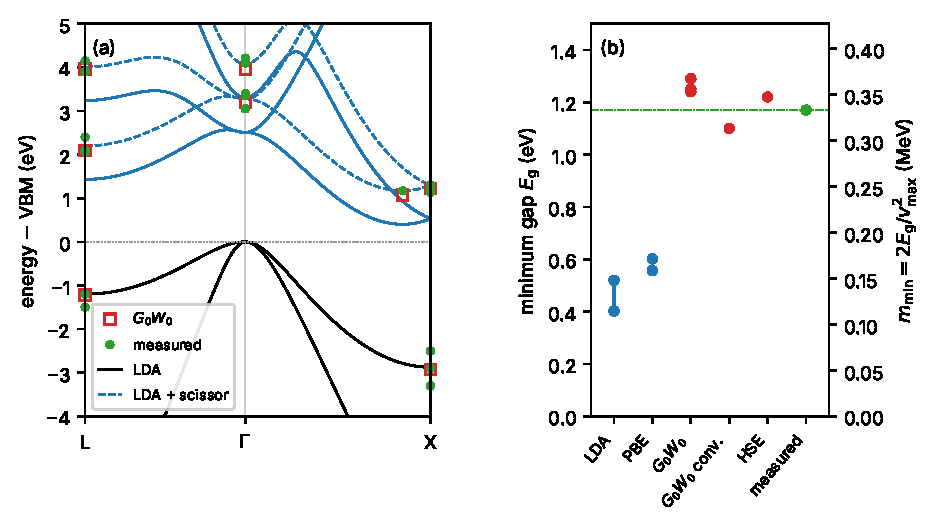
\includegraphics[width=\linewidth]{figures/ch03/fig3_8.pdf}
  \caption{The gap of silicon in density-functional theory, in quasiparticle calculations and in experiment. (a)~Solid: Kohn--Sham bands in the local-density approximation along $\mathrm{L}$--$\mathrm{\Gamma}$--$\mathrm{X}$, valence black and conduction blue, from the VBM; Slater exchange and Perdew--Zunger correlation~\cite{perdew1981self}, in the plane-wave calculation of \cref{app:E.1} (SG15 norm-conserving pseudopotential, \SI{60}{Ry}, $12^3$ grid, $a = \SI{5.431}{\angstrom}$, no spin--orbit coupling)~\cite{giannozzi2017advanced,hamann2013optimized,schlipf2015optimization}. Their minimum gap is \SI{0.40}{eV} at $0.848\,(2\pi/a)$; it changes by less than \SI{1}{meV} at \SI{80}{Ry} or on a $16^3$ grid, and the conduction states at $\mathrm{\Gamma}$, $\mathrm{X}$ and $\mathrm{L}$ lie at 2.51, 0.53 and \SI{1.43}{eV}. The pseudopotential was generated with PBE; a consistent LDA potential would raise the gap to about \SI{0.50}{eV}, close to the tabulated LDA value of \SI{0.52}{eV} (\cref{tab:E-gw}). Dashed: the same conduction bands shifted up by $\Delta_{\mathrm{scis}} = \SI{0.77}{eV}$, so that the minimum gap equals the measured \SI{1.17}{eV}. Squares: one-shot $G_0W_0$ quasiparticle energies, and circles: measured energies (all values listed there), both as given in Ref.~\cite[Tables~II and VI]{rideau2006strained}, at $\mathrm{\Gamma}$, $\mathrm{L}$, $\mathrm{X}$ and the conduction-band minimum. The $G_0W_0$ calculation is a different one from the LDA bands shown and includes spin--orbit coupling, whose splittings, below \SI{0.05}{eV}, are not resolved. (b)~Minimum gap from LDA~\cite[Table~I]{aryasetiawan1998gw} and from the LDA bands of panel (a), from PBE at the measured lattice constant (\cref{fig:3-si-bands}) and at the PBE lattice constant (\cref{we:E-si-bands}), from $G_0W_0$ calculations started from LDA~\cite{hybertsen1986electron,godby1988self,rohlfing1993quasiparticle} as collected in Ref.~\cite[Table~I]{aryasetiawan1998gw} and converged~\cite[Sect.~IV\,C]{klimes2014predictive}, from the hybrid functional HSE~\cite[Table~I]{lucero2012improved}, and measured at low temperature~\cite[Eq.~(11)]{ramanathan2020ionization}. Right axis: the threshold mass $m_{\mathrm{min}} = 2\Eg/v_{\mathrm{max}}^2$ of \cref{eq:1.3-mmin}, $v_{\mathrm{max}} = 2.650\times10^{-3}$.}
  \label{fig:3-si-qp}
\end{figure}

Why are quasiparticle gaps larger than Kohn--Sham gaps, and smaller than Hartree--Fock ones? A physical picture follows from what each theory lets the other electrons do, as anticipated above. In Hartree--Fock, an electron in an occupied state is bound by the exchange with the other electrons of its spin, while an electron in an empty state has no exchange with itself; this difference, of order the exchange energy of several eV, opens the gap. But the other electrons are frozen. A real added electron repels the electrons around it and polarizes the crystal, and the polarization lowers its energy; a real hole attracts them, with the same effect on the energy to create it. Both corrections close the gap. They come from screening, which at long range cuts the exchange interaction down by $1/\varepsilon_\infty$, a factor of 12 in silicon. The result is screened exchange: the exchange of Hartree--Fock with the bare Coulomb interaction replaced, at long range, by the interaction screened by $\varepsilon_\infty$, together with the energy of the polarization cloud that the particle carries along, the Coulomb-hole term of \cref{app:E.3}. A local Kohn--Sham potential is at the other extreme. It acts in the same way on occupied and empty states, and does not contain the discontinuity in the cost of adding an electron. The quasiparticle gap lies between the two limits, and in a strongly screening semiconductor it lies closer to the Kohn--Sham one. The $GW$ approximation of \cref{sec:4.8} makes this picture quantitative: its self-energy is the exchange with the dynamically screened interaction $W^{\mathrm{scr}}$. Started from LDA, it gives the silicon gap at 1.24 to \SI{1.29}{eV} in the calculations of the 1980s and early 1990s~\cite{hybertsen1986electron,godby1988self}\cite[Table~I]{aryasetiawan1998gw}, and at \SI{1.10}{eV} when converged with current methods~\cite[Sect.~IV\,C]{klimes2014predictive}. Hybrid functionals use the same idea crudely, with a fixed fraction of the Fock exchange; HSE gives \SI{1.22}{eV} (\cref{fig:3-si-qp}(b)).

The gap error reaches every quantity of a dark-matter rate that depends on energy differences across the gap. The threshold mass $m_{\mathrm{min}} = 2\Eg/v_{\mathrm{max}}^2$ is proportional to the gap, and the minimum pair energy $E_{\mathrm{min}}(\vect{q})$ of \cref{eq:3.3-Emin} moves with the conduction bands. Effective masses at a direct gap scale with it through \cref{eq:3.3-kane2}, as the Kane estimate of \cref{sec:3.3} shows for GaAs. The silicon valleys are less sensitive, since their mass comes from distant bands, and the PBE longitudinal mass is only \SI{4}{\percent} too heavy (\cref{app:E.1}). The screening is affected as well. Every transition contributes to $\varepsilon_\infty - 1$ more strongly the smaller its energy, and a gap that is too small makes the screening too strong, 13.04 against 11.7 in the PBE calculation of \cref{app:E.1}. The in-medium screening of \cref{chap:4} suppresses a rate by $|\varepsilon|^{-2}$, and it then suppresses it too much. A computed rate is therefore only as good as the gap behind it. Where the gap is measured, it can be imposed; where it is not, the spread of the methods in \cref{fig:3-si-qp}(b), about \SI{0.1}{eV} in silicon among calculations that treat the gap seriously, is a theory uncertainty of the threshold.

\subsection{The scissor shift}

Since the LDA or PBE conduction bands of silicon are nearly right in shape, the cheapest repair is to move them. The \emph{scissor shift} raises every conduction band by the same amount $\Delta_{\mathrm{scis}}$ and leaves the valence bands and all the states as they are:
\begin{equation}
  H^{\mathrm{s}}_{\vect{k}} = H_{\vect{k}} + \Delta_{\mathrm{scis}}\,P_{\mathrm{c}}(\vect{k}), \qquad
  P_{\mathrm{c}}(\vect{k}) = \sum_c|u_{c\vect{k}}\rangle\langle u_{c\vect{k}}| ,
  \label{eq:3.4-scissor}
\end{equation}
with $H_{\vect{k}}$ the Bloch Hamiltonian \cref{eq:3.2-Hk} of the Kohn--Sham potential and the sum over all conduction bands. Its eigenstates are those of $H_{\vect{k}}$, with eigenvalues $\varepsilon_{v\vect{k}}$ and $\varepsilon_{c\vect{k}} + \Delta_{\mathrm{scis}}$. The shift is chosen to bring the computed gap to a measured or a quasiparticle one: for the PBE calculation of \cref{we:E-si-bands}, $\Delta_{\mathrm{scis}} = 1.170 - 0.602 = \SI{0.568}{eV}$ at the PBE lattice constant, and \SI{0.613}{eV} at the measured one. Against full quasiparticle calculations, a rigid shift is good to about \SI{0.1}{eV} across the bands in silicon, and to 0.2 and \SI{0.4}{eV} in GaAs and diamond~\cite{godby1988self}\cite[Sect.~V\,B]{aryasetiawan1998gw}.

What does the shift do to the ingredients of a rate? Energies and the density vertex are easy. Every interband energy grows by $\Delta_{\mathrm{scis}}$, and so does $E_{\mathrm{min}}(\vect{q})$ at every $\vect{q}$. The density vertex $\rho_{cv}(\vect{k}, \vect{q})$ of \cref{eq:3.2-rho} is an overlap of states, and the states do not change. The velocity matrix elements are less obvious. $P_{\mathrm{c}}$ is a nonlocal operator, and the velocity, $\ii[H, \vect{r}]$, picks up a commutator with it. By \cref{eq:3.2-dHk}, the velocity matrix elements of $H^{\mathrm{s}}$ are those of $\nabla_{\vect{k}}H^{\mathrm{s}}_{\vect{k}}$. This operator contains the derivative of the projector,
\begin{equation*}
  \nabla_{\vect{k}}H^{\mathrm{s}}_{\vect{k}} = \nabla_{\vect{k}}H_{\vect{k}} + \Delta_{\mathrm{scis}}\sum_{c'}\Bigl(|\nabla_{\vect{k}}u_{c'\vect{k}}\rangle\langle u_{c'\vect{k}}| + |u_{c'\vect{k}}\rangle\langle\nabla_{\vect{k}}u_{c'\vect{k}}|\Bigr) .
\end{equation*}
Between a conduction state $c$ and a valence state $v$ at the same $\vect{k}$, the first term in the bracket contributes $\sum_{c'}\langle u_c|\nabla_{\vect{k}}u_{c'}\rangle\langle u_{c'}|u_v\rangle = 0$, since conduction and valence states are orthogonal. The second contributes $\langle\nabla_{\vect{k}}u_c|u_v\rangle$, the term $c' = c$ of $\sum_{c'}\langle u_c|u_{c'}\rangle\langle\nabla_{\vect{k}}u_{c'}|u_v\rangle$. Differentiating $\langle u_c|u_v\rangle = 0$ gives $\langle\nabla_{\vect{k}}u_c|u_v\rangle = -\langle u_c|\nabla_{\vect{k}}u_v\rangle$, and \cref{eq:3.2-dudk} gives $\langle u_c|\nabla_{\vect{k}}u_v\rangle = \vect{v}_{cv}/(\varepsilon_{v\vect{k}} - \varepsilon_{c\vect{k}})$. Altogether,
\begin{equation*}
  \vect{v}^{\mathrm{s}}_{cv}(\vect{k}) = \vect{v}_{cv}(\vect{k}) - \Delta_{\mathrm{scis}}\,\frac{\vect{v}_{cv}(\vect{k})}{\varepsilon_{v\vect{k}} - \varepsilon_{c\vect{k}}}
  = \vect{v}_{cv}(\vect{k})\Bigl(1 + \frac{\Delta_{\mathrm{scis}}}{\varepsilon_{c\vect{k}} - \varepsilon_{v\vect{k}}}\Bigr) .
\end{equation*}
Between two conduction states the two terms of the bracket give
\begin{equation*}
  \Delta_{\mathrm{scis}}\bigl(\langle u_c|\nabla_{\vect{k}}u_{c'}\rangle + \langle\nabla_{\vect{k}}u_c|u_{c'}\rangle\bigr) = \Delta_{\mathrm{scis}}\nabla_{\vect{k}}\langle u_c|u_{c'}\rangle = 0 ,
\end{equation*}
and between two valence states the projector does not act, so neither changes.
\begin{keyresult}[Scissor rescaling of the velocity]
Under the scissor shift \cref{eq:3.4-scissor}, energies and states transform as
\begin{equation}
  \begin{gathered}
  \varepsilon_{c\vect{k}} \to \varepsilon_{c\vect{k}} + \Delta_{\mathrm{scis}}, \qquad \rho_{mn}(\vect{k}, \vect{q}) \to \rho_{mn}(\vect{k}, \vect{q}), \\
  \vect{v}_{cv}(\vect{k}) \to \vect{v}_{cv}(\vect{k})\,\frac{\varepsilon_{c\vect{k}} - \varepsilon_{v\vect{k}} + \Delta_{\mathrm{scis}}}{\varepsilon_{c\vect{k}} - \varepsilon_{v\vect{k}}} ,
  \end{gathered}
  \label{eq:3.4-vscis}
\end{equation}
while the velocity matrix elements within the valence bands and within the conduction bands, the group velocities included, are unchanged.
\end{keyresult}
The interband velocity grows in proportion to the transition energy, and the optical limit \cref{eq:3.2-optical} shows why it must. The vertex $\rho_{cv} = \vect{q}\cdot\vect{v}_{cv}/(\varepsilon_{c\vect{k}} - \varepsilon_{v\vect{k}})$ is fixed because the states are fixed, so a larger denominator needs a larger numerator. The same follows from \cref{eq:3.2-r}: the position matrix element between the unchanged states stays the same, and the velocity is $\ii$ times the energy difference times it. \Cref{app:E.3} extends the rescaling to quasiparticle corrections that differ from state to state. At the direct gap of silicon at $\mathrm{\Gamma}$, \SI{2.55}{eV} in the PBE calculation at its own lattice constant, the shift of \SI{0.568}{eV} multiplies the velocity by $3.12/2.55 = 1.22$ and its square by 1.50. An absorption rate built from the shifted energies but the unshifted velocities comes out too small by that factor.

A scissor keeps the order of the Kohn--Sham bands, and where a functional gets that order wrong, as PBE does in germanium, whose conduction state at $\mathrm{\Gamma}$ falls below the $\mathrm{L}$ valleys, no rigid shift repairs it (\cref{app:E.1}). It leaves the states unchanged, while the energies of all transitions rise, so that the $f$-sum rule of \cref{sec:4.3}, a sum of transition energies times $|\rho_{cv}|^2$, exceeds its exact value by $\Delta_{\mathrm{scis}}\sum_c|\rho_{cv}|^2$, the signature of a nonlocal operator in the Hamiltonian (\cref{app:E.3}). And a scissor to a measured gap imports everything the measurement contains, including the renormalization of the gap by the zero-point motion of the lattice (\cref{sec:13.7}), which must then not be added a second time.

\begin{workedexample}{The silicon threshold mass from computed gaps}\label{we:3-mmin-gap}
The threshold mass of \cref{eq:1.3-mmin} is $m_{\mathrm{min}} = 2\Eg/v_{\mathrm{max}}^2$, with $v_{\mathrm{max}}^2 = \num{7.023e-6}$. For the gaps of \cref{fig:3-si-qp}(b),
\begin{equation*}
  \begin{aligned}
  &\text{LDA, \SI{0.52}{eV}:} & m_{\mathrm{min}} &= \frac{2\times\SI{0.52}{eV}}{\num{7.023e-6}} = \SI{0.148}{MeV}, \\
  &\text{PBE, \SI{0.602}{eV}:} & m_{\mathrm{min}} &= \SI{0.171}{MeV}, \\
  &\text{$G_0W_0$, 1.10 to \SI{1.29}{eV}:} & m_{\mathrm{min}} &= 0.313 \text{ to } \SI{0.367}{MeV}, \\
  &\text{measured, \SI{1.17}{eV}:} & m_{\mathrm{min}} &= \SI{0.333}{MeV}.
  \end{aligned}
\end{equation*}
Taken at face value, an LDA band structure lowers the threshold mass by a factor $1.17/0.52 = 2.25$, to less than half its true value. A projection computed with uncorrected bands would claim reach between 0.148 and \SI{0.333}{MeV}, where a silicon detector has none.

The bound of \cref{we:3-kc}, which requires the particle to deposit the gap at the conduction-band minimum $k_{\mathrm{c}} = \SI{1.94}{keV}$, responds much less. With the LDA gap,
\begin{equation*}
  \mchi = \frac{k_{\mathrm{c}}^2}{2(k_{\mathrm{c}}v_{\mathrm{max}} - \Eg)} = \frac{(\SI{1940}{eV})^2}{2\,(\SI{5.14}{eV} - \SI{0.52}{eV})} = \SI{0.407}{MeV},
\end{equation*}
against \SI{0.474}{MeV} with the measured gap. Near $k_{\mathrm{c}}$ the momentum needed to reach the valley, not the energy, limits light particles, and the error of the gap is diluted by the kinetic term $k_{\mathrm{c}}v_{\mathrm{max}} = \SI{5.14}{eV}$. Where the true threshold lies between these bounds is a question for \cref{sec:13.1}. Both bounds, however, move down when the gap is too small.

Once the gap is fixed by a scissor to the measured value, the remaining uncertainty is that of the measurement and of its temperature, a few meV. Without a measurement, the spread of \SI{0.1}{eV} among quasiparticle methods translates through $\delta\ln m_{\mathrm{min}} = \delta\ln\Eg$ (\cref{sec:1.3-edge}) into $0.1/1.17 = \SI{8.5}{\percent}$ in $m_{\mathrm{min}}$, more than the \SI{6}{\percent} that the uncertainty of the escape speed contributes. Just above the edge, where the halo supply grows by orders of magnitude over a factor of two in mass, such a shift changes the expected rate by large factors.
\end{workedexample}

The Kohn--Sham bands, corrected for the gap, are the input of every electronic rate in the rest of the book. They come from a calculation with pseudopotentials, whose states are smooth where the true ones oscillate near the nuclei, and the density vertex at the momentum transfers that dark matter reaches depends on exactly those oscillations. \Cref{sec:3.5} restores them.

\printbibliography[heading=subbibliography]
